%!TEX encoding = UTF-8 Unicode
\documentclass[10pt]{article}
\usepackage[a4paper, total={6in, 8in}]{geometry}
\usepackage[usenames,dvipsnames,svgnames,table]{xcolor} % usenames : 16 basic colors,  dvipsnames : other 68 colors, svgnames : another 150 colors. It is used instead of \usepackage{color}. Can find descriptions for color in xcolor package. 

% algorithm
% (1) rename require/ensure https://en.wikibooks.org/wiki/LaTeX/Algorithms#Typesetting_using_the_algorithmic_package 
\usepackage{algorithm}
\usepackage{algorithmic}
\floatname{algorithm}{Algorithm}
\renewcommand{\algorithmicrequire}{\textbf{Input:}}
\renewcommand{\algorithmicensure}{\textbf{Output:}}

% table management
\usepackage{longtable}
\usepackage{hhline}
\usepackage{float}
\newfloat{algorithm}{tb}{lop}

\usepackage{enumitem} % for \begin{description}
\usepackage{rotfloat} % For [H] option in sidewaystable
\usepackage{graphicx}
\usepackage{epsfig}
\usepackage{amssymb, amsmath, amsthm}
\usepackage{verbatim}
\usepackage{hyperref}
\usepackage{natbib}
\usepackage{authblk}
%\usepackage{kotex}
\usepackage{multirow}
%\usepackage[colorlinks]{hyperref} % it is needed for todonotes package. 
%\usepackage[colorinlistoftodos, textsize=scriptsize]{todonotes} % For making notes. disable option removes all notes. 
\usepackage{subcaption} % for \begin{subtable}
\usepackage{array}
\newcolumntype{L}{>{\centering\arraybackslash}m{0.1\linewidth}}

\renewcommand{\baselinestretch}{1.25}

\newtheorem{theorem}{Theorem}[section]
\newtheorem{lemma}[theorem]{Lemma}
\newtheorem{proposition}[theorem]{Proposition}
\newtheorem{corollary}[theorem]{Corollary}
\newtheorem{fact}[theorem]{Fact}
\newtheorem{example}{Example}[section]
\newtheorem{definition}{Definition}






%\newenvironment{proof}[1][Proof]{\begin{trivlist}
%\item[\hskip \labelsep {\bfseries #1}]}{\end{trivlist}}
%\newenvironment{definition}[1][Definition]{\begin{trivlist}
%\item[\hskip \labelsep {\bfseries #1}]}{\end{trivlist}}
%\newenvironment{remark}[1][Remark]{\begin{trivlist}
%\item[\hskip \labelsep {\bfseries #1}]}{\end{trivlist}}



%\newcommand{\qed}{\nobreak \ifvmode \relax \else
%      \ifdim\lastskip<1.5em \hskip-\lastskip
%      \hskip1.5em plus0em minus0.5em \fi \nobreak
%      \vrule height0.75em width0.5em depth0.25em\fi}

%\def\qed{\space$\Box$ \par \vspace{.15in}}

% ***************************************************************
% Changed by Kisung You
\DeclareMathOperator*{\argmin}{argmin}
\DeclareMathOperator*{\argmax}{argmax}
\newcommand{\todokl}{\todo[inline,color=lime]}


\newcommand{\Exp}{\textrm{Exp}}
\newcommand{\Log}{\textrm{Log}}

\newcommand{\bfu}{\mathbf{u}}
\newcommand{\bfv}{\mathbf{v}}
\newcommand{\bfw}{\mathbf{w}}
\newcommand{\bfx}{\mathbf{x}}
\newcommand{\bfy}{\mathbf{y}}
\newcommand{\bfz}{\mathbf{z}}
\newcommand{\bfmu}{\boldsymbol{\mu}}


\newcommand{\bfX}{\mathbf{X}}
\newcommand{\bfY}{\mathbf{Y}}
\newcommand{\bfZ}{\mathbf{Z}}
\newcommand{\bfTheta}{\mathbf{\Theta}}
\newcommand{\bfGamma}{\mathbf{\Gamma}}


\newcommand{\bbS}{\mathbb{S}}
\newcommand{\bbR}{\mathbb{R}}
\newcommand{\bbX}{\mathbb{X}}
\newcommand{\bbRpos}{\mathbb{R}^+}

\newcommand{\calM}{\mathcal{M}}

\newcommand{\rmE}{\textrm{E}}
\newcommand{\rmP}{\textrm{P}}

% density functions
\newcommand{\fvMF}{f_{\textrm{vMF}}}
\newcommand{\fSN}{f_{\textrm{SN}}}
\newcommand{\fSL}{f_{\textrm{SL}}}

% MLE
\newcommand{\mleloc}{\hat{\bfmu}_{\textrm{MLE}}}
\newcommand{\mlescale}{\hat{\sigma}_{\textrm{MLE}}}

% others
\newcommand{\Frechet}{Fr\'{e}chet }

% ***************************************************************

\parindent=15pt
\textheight 22cm \textwidth  16.5cm \oddsidemargin 0mm \topmargin     5mm
\headheight    0mm


\begin{document}
	
\title{On the spherical Laplace distribution}
\author[1]{Kisung You}
\author[1]{Dennis Shung}
\affil[1]{Department of Internal Medicine, Yale School of Medicine}
%\affil[2]{Department of Computer Science, Yale University}
%\affil[3]{Program in Applied Mathematics, Yale University}
%\affil[4]{Program in Computational Biology and Bioinformatics, Yale University}
\date{}

\maketitle
\begin{abstract}
The von Mises-Fisher (vMF) distribution has long been a mainstay for inference with data on the unit hypersphere in directional statistics. The performance of statistical inference based on the vMF distribution, however, may suffer when there are significant outliers and noise in the data. Based on an analogy of the median as a robust measure of central tendency and its relationship to the Laplace distribution, we proposed the spherical Laplace (SL) distribution, a novel probability measure for modelling directional data. We present a sampling scheme and theoretical results on maximum likelihood estimation. We derive efficient numerical routines for parameter estimation in the absence of closed-form formula. An application of model-based clustering is considered under the finite mixture model framework. Our numerical methods for parameter estimation and clustering are validated using simulated and real data experiments.
\end{abstract}

%Keywords: Directional statistics, Model-based clustering, Robust statistics, Spherical Laplace distribution.


%%%%%%%%%%%%%%%%%%%%%%%%%%%%%%%%%%%%%%%%%%%%%%%%%%%%%%%%%%%%%%%%%%%%%%%%%%%%%%%%%%%%%%%%%%%%%%%%%%%%%%
\section{Introduction}\label{sec1:intro}

A prominent discipline in modern data science is to learn from data equipped with certain geometric constraints. The program often assumes that data reside on Riemannian manifolds \cite{lee_1997_RiemannianManifoldsIntroduction} and has attracted much attention over the last decades in both theoretical foundation \cite{pennec_2006_IntrinsicStatisticsRiemannian, bhattacharya_2012_NonparametricInferenceManifolds, patrangenaru_2016_NonparametricStatisticsManifolds} and practical applications across many fields including  computer vision \cite{bissacco_2001_RecognitionHumanGaits, aggarwal_2004_SystemIdentificationApproach} and medical image analysis  \cite{pennec_2020_RiemannianGeometricStatistics, fletcher_2009_GeometricMedianRiemannian, you_2021_RevisitingRiemannianGeometry}. In statistics, the relevant research area has long been known as directional statistics  \cite{mardia_2000_DirectionalStatistics, ley_2017_ModernDirectionalStatistics} whose objects of interests include directions, axes, and rotations. Especially, directions seem to take the largest portion in the field for its popularity as a number of applications involve observations on the unit hypersphere, which is a model manifold of constant positive curvature. 

An off-the-shelf choice of probability measure on the unit hypersphere is the von Mises-Fisher (vMF) distribution \cite{fisher_1953_DispersionSphere, mardia_2000_DirectionalStatistics}, which is a location-scale family distribution that has higher concentration of mass near a mean direction. Recently, the spherical normal (SN) distribution \cite{hauberg_2018_DirectionalStatisticsSpherical} was proposed as an alternative by adopting the geodesic distance on the unit hypersphere. Both distributions are Gaussian-like laws since they are defined using negated squared distances to their location parameters within an exponential function. For both distributions, it is straightforward to see that the maximum likelihood estimate of a location parameter corresponds to the quantity called \Frechet mean \cite{kendall_1990_ProbabilityConvexityHarmonic}, which is a minimizer of sum of squared distances. 


While these distributions may play an important role in statistical inference, their performance may deteriorate when there exist outliers or noise of large magnitude. In classical robust statistics \cite{huber_1981_RobustStatistics}, it is well acknowledged that the median is a robust measure of central tendency. This has been translated in the field of statistics on manifolds to replace \Frechet mean with \Frechet median, which minimizes sum of distances  \cite{fletcher_2009_GeometricMedianRiemannian, arnaudon_2013_MediansMeansRiemannian}. Hence, it is natural to ask what distribution is related to the concept of \Frechet median on the unit hypersphere as the vMF and SN distributions to the \Frechet mean. 

This motivates our paper to propose the spherical Laplace (SL) distribution. As its name entails, the SL distribution generalizes the Laplace distribution on the real line onto the unit hypersphere by defining its density function using  a scaled distance to a mean location rather than squared distance. A leading contribution of this paper is to establish the SL distribution and derive an explicit, simplified form of a normalizing constant amicable for numerical approximation. We also consider a rejection-based sampling scheme to draw random samples from the SL distribution. 

Another class of our contribution is on parameter estimation in the sense of maximum likelihood, which is one of the fundamental tasks for statistical inference. We show that under mild support conditions the SL distribution admits unique parameter estimates. Since the maximum likelihood estimates are  solutions of nonlinear equations, we present algorithms for numerical optimization of the parameters. 

We consider model-based clustering \cite{bouveyron_2019_ModelbasedClusteringClassification} as a major application of the SL distribution. We employ the finite mixture model \cite{mclachlan_2019_FiniteMixtureModels}, which is also a major tool for density estimation, for model-based clustering of data on the unit hypersphere using the SL distribution as its components. Computation for the SL mixture is heavily dependent on a generalized version of the parameter estimation algorithms where observations are given fixed weights. We present computational pipeline in detail for the SL mixture in a similar fashion to its predecessors \cite{banerjee_2005_ClusteringUnitHypersphere, hornik_2014_MovMFPackageFitting}. Computational apparatus for the SL distribution is implemented in an \textsf{R} package called \texttt{Riemann}, which is available on CRAN (\url{https://CRAN.R-project.org/package=Riemann}) and GitHub (\url{https://github.com/kisungyou/Riemann}).


The rest of this paper is organized as follows. We start by introducing rudimentary background on geometry of hypersphere and describing how vMF and SN distributions are related in Section \ref{sec2:background}. Section \ref{sec3:SL} presents the SL distribution along with a rejection sampler and theoretical results regarding maximum likelihood estimation. We present numerical routines for parameter estimation in Section \ref{sec4:parameter}. In Section \ref{sec5:clustering}, the SL mixture is presented in technical details. The distribution and proposed algorithms are validated via simulated and real data experiments in Section \ref{sec6:experiments}. We conclude by discussing potential issues and a list of topics for future studies in Section \ref{sec7:conclusion}. 




%%%%%%%%%%%%%%%%%%%%%%%%%%%%%%%%%%%%%%%%%%%%%%%%%%%%%%%%%%%%%%%%%%%%%%%%%%%%%%%%%%%%%%%%%%%%%%%%%%%%%%
\section{Background}\label{sec2:background}

We start this section by introducing notations throughout the paper. Let $\bbS^p = \lbrace \bfx \in \bbR^{p+1}: \|\bfx\| = 1 \rbrace$ be a $p$-dimensional unit sphere in a $(p+1)$-dimensional Euclidean space $\bbR^{p+1}$ where $\| \cdot \|$ is the standard $\ell_2$ norm. For a metric space $(\bbX, \delta)$, an open ball of radius $\epsilon > 0$ centered at $\bfx \in \bbX$ is denoted as $B(\bfx, \epsilon) = \lbrace \bfy \in \bbX~|~ \delta(\bfx, \bfy) < \epsilon \rbrace$. For two points $\bfx, \bfy \in \bbS^p$, the distance $d(\bfx, \bfy)$ is reserved to denote the geodesic or shortest-path distance on a sphere. A superscript $^{(t)}$ indicates an object at iteration $t$. The set of positive real numbers is denoted as $\bbRpos$. 

\subsection{Geometry of hypersphere}

The unit hypersphere is a model space for a simply connected manifold of constant positive curvature \cite{carmo_1992_RiemannianGeometry, lee_1997_RiemannianManifoldsIntroduction}. We review basic properties of the unit sphere as a Riemannian manifold and explicit forms of computational operations \cite{absil_2008_OptimizationAlgorithmsMatrix}.

For some $\bfx \in \bbS^p$, the tangent space is characterized as $T_\bfx \bbS^p = \lbrace \bfz \in \bbR^{p+1}~|~ \langle \bfx, \bfz \rangle = 0 \rbrace $ with a standard inner product $\langle \cdot, \cdot \rangle$.  The Riemannian metric for $\bbS^p$ is a canonical metric, i.e., $g_\bfx (\bfu, \bfv) = \langle \bfu, \bfv\rangle$ for all $\bfu, \bfv \in T_\bfx \bbS^p$. The shortest path connecting any two points $\bfx, \bfy \in \bbS^p$ is along the great circle in that the geodesic distance is given by $d(\bfx, \bfy) = \text{arccos}(\langle \bfx, \bfy \rangle)$. Given a pair $(\bfx, \bfu) \in \calM \times T_\bfx \calM$ for some Riemannian manifold $\calM$, there exists a unique geodesic $\gamma : [0,1] \rightarrow \calM$ such that $\gamma (0) = \bfx$ and $\gamma' (0) = \bfu$. An exponential map is defined by $\Exp_\bfx (\bfu) = \gamma ( 1)$, which maps a vector in some tangent space to the manifold itself whose inverse is called a logarithmic map, as shown in \figurename \ref{fig:TwoMaps}. When $\calM = \bbS^p$, two maps are endowed with explicit formula. Define an operator  $\textrm{Proj}_\bfx (\bfz) = \bfz - \langle \bfx, \bfz \rangle \bfx$ that projects some vector $\bfz \in \bbR^{p+1}$ onto the tangent space $T_\bfx \bbS^p$. For $\bfx, \bfy \in \bbS^p$ and $\bfu \in T_\bfx \bbS^p$, we have the following expressions;
\begin{subequations}
	\begin{align}
	\textrm{(exponential map)}\quad &\quad \text{Exp}_\bfx (\bfu) = \cos (\|\bfu\|) x + \frac{\sin(\|\bfu\|)}{\|\bfu\|} \bfu, \label{eq:map_exponential} \\
	\textrm{(logarithmic map)}\quad &\quad \text{Log}_\bfx (\bfy) = \frac{d(\bfx,\bfy)}{\|\text{Proj}_\bfx (\bfy-\bfx)\|} \text{Proj}_\bfx (\bfy-\bfx). \label{eq:map_logarithmic}
	\end{align}	
\end{subequations}
An exponential map, by its construction, is only locally defined. The injectivity radius $\textrm{inj}(\calM)$ of a manifold $\calM$ is a maximal radius of a geodesic ball where the exponential map is well-defined and a diffeomorphism, which is $\pi$ for the unit hypersphere. 



\begin{figure}[ht]
	\centering
	
\includegraphics[width=0.4\linewidth]{figures/geometry-eps-converted-to.pdf}
	\caption{Visual representation of exponential ({\color{red}\bf red}) and logarithmic ({\color{blue} \bf blue}) maps on a Riemannian manifold $\calM$ for some points $\bfx, \bfy \in \calM$ and a tangent vector $\bfu \in T_\bfx \calM$. }
	\label{fig:TwoMaps}
\end{figure}




\subsection{The von Mises-Fisher and spherical normal distributions}

On the $p$-dimensional unit hypersphere, the vMF is one of the most popular distributions as an exponential family distribution that has seen many applications  \cite{banerjee_2005_ClusteringUnitHypersphere, bhattacharya_2012_NonparametricBayesClassification, gopal_2014_MisesfisherClusteringModels}. Parametrized by two parameters for  location $\bfmu \in \bbS^p$ and scale $\kappa \in \bbRpos$, the vMF distribution has the following density function of the form $\fvMF (\bfx~|~ \boldsymbol{\mu}, \kappa) \propto \exp (\kappa \bfx^\top \bfmu)$. One observation is that the density is characterized by the square of Euclidean distance,
\begin{equation}\label{eq:vMF_squared}
\exp \left( -\frac{\kappa}{2} \|\bfx - \bfmu\|^2 \right) = \exp \left( -\frac{\kappa}{2} \left\lbrace \bfx^\top \bfx  - 2\bfx^\top \bfmu + \bfmu^\top \bfmu \right\rbrace \right) = C(\kappa) \exp (\kappa \bfx^\top \bfmu),
\end{equation}
where the constant $C(\kappa)$ does not affect the term inside an exponential since $\|\bfx\|=\|\bfmu\|=1$. Therefore, we may roughly consider the vMF distribution as a direct adaptation of the isotropic Gaussian distribution onto the unit hypersphere. 


It is natural to question whether the use of standard Euclidean distribution in defining a probability measure on the constrained domain of hypersphere is appropriate. This led to a recent proposal of the SN distribution to replace the Euclidean norm with the geodesic distance. For an isotropic version of the SN distribution, the density function, parametrized by
location $\bfmu \in \bbS^p$ and concentration $\lambda \in \bbRpos$ parameters, is of the following form
\begin{equation}
\fSN (\bfx~|~\bfmu,\lambda) \propto \exp \left(-\frac{\lambda}{2} d^2 (\bfx, \bfmu)\right).
\end{equation}
We close this section by discussing the connection between vMF and SN distributions. As we observed in \eqref{eq:vMF_squared}, both laws are parametrized by scaled square of some distances from a location parameter. In the literature of statistics on manifolds, these two formulations correspond to the dichotomy of \textit{intrinsic} and \textit{extrinsic} frameworks \cite{bhattacharya_2012_NonparametricInferenceManifolds}. Roughly speaking, the intrinsic approach measures dissimilarity of two points on a manifold by the shortest-path geodesic joining the two, while the extrinsic framework uses a standard norm after equivariant embedding of the data on manifold onto the Euclidean space \cite{wasserman_1969_EquivariantDifferentialTopology}. Therefore, vMF and SN distributions may be regarded as extrinsic and intrinsic Gaussian-like probability laws on the sphere, respectively. Hence, this motivates to define a spherical extension of the Laplace distribution by reducing the order of exponent from the SN density function from 2 to 1. 

%%%%%%%%%%%%%%%%%%%%%%%%%%%%%%%%%%%%%%%%%%%%%%%%%%%%%%%%%%%%%%%%%%%%%%%%%%%%%%%%%%%%%%%%%%%%%%%%%%%%%%
\section{The spherical Laplace distribution}\label{sec3:SL}
\subsection{Definition}

We propose the spherical Laplace (SL) distribution, which is an isotropic location-scale family distribution on the unit hypersphere $\bbS^p$ of $p\geq 1$. 

\begin{definition} Let $\bfmu \in \bbS^p$ and $\sigma \in \bbRpos$ be location and scale parameters, respectively. Density function of the SL distribution is defined by
	\begin{equation*}
	\fSL (\bfx~|~ \boldsymbol{\mu}, \sigma) = \frac{1}{C_p (\bfmu, \sigma)} \exp \left( -\frac{d(\bfx, \bfmu)}{\sigma} \right),
	\end{equation*}
	for a normalizing constant $C_p (\bfmu, \sigma)$,
	\begin{equation}\label{eq:normalizing_constant_full}
	C_p (\bfmu, \sigma) = \int_{\bbS^p} \exp \left( -\frac{d(\bfx, \bfmu)}{\sigma} \right) d\bfx.
	\end{equation}
\end{definition}
The scale parameter quantifies the degree of dispersion as shown in \figurename \ref{fig:three_densities}, where a small $\sigma$ leads to concentrated mass around $\bfmu$ and a large $\sigma$ leads to largely dispersed distribution of the mass.



It is trivial to observe that \eqref{eq:normalizing_constant_full} is well defined. The integrand is a smooth,  bounded function due to the fact that $\sigma$ is strictly positive and $d(\bfx, \bfmu)$ is bounded in $(0,\pi)$. Since the domain is compact, the integral is finite. However, evaluation of \eqref{eq:normalizing_constant_full} involves multidimensional integration over the constrained domain, which makes practical usage of the distribution prohibitive. Although a closed-form formula is not available, we show in the following proposition that the expression for normalizing constant can be transformed into a single-variable integration over the bounded domain. 

\begin{figure}[ht]
	\centering
	\begin{subfigure}[b]{0.3\textwidth}
		\centering
		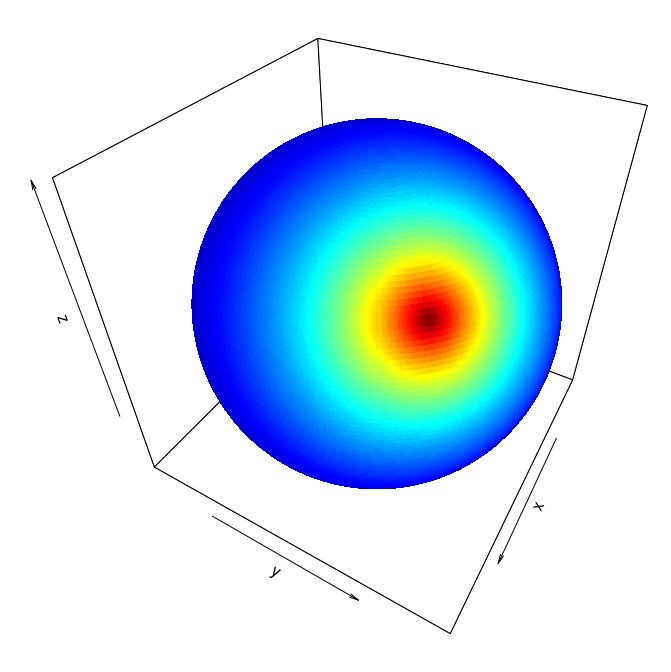
\includegraphics[width=\textwidth]{figures/density_case1.png}
		\caption{$\sigma=0.5$}
	\end{subfigure}
	\hfill
	\begin{subfigure}[b]{0.3\textwidth}
		\centering
		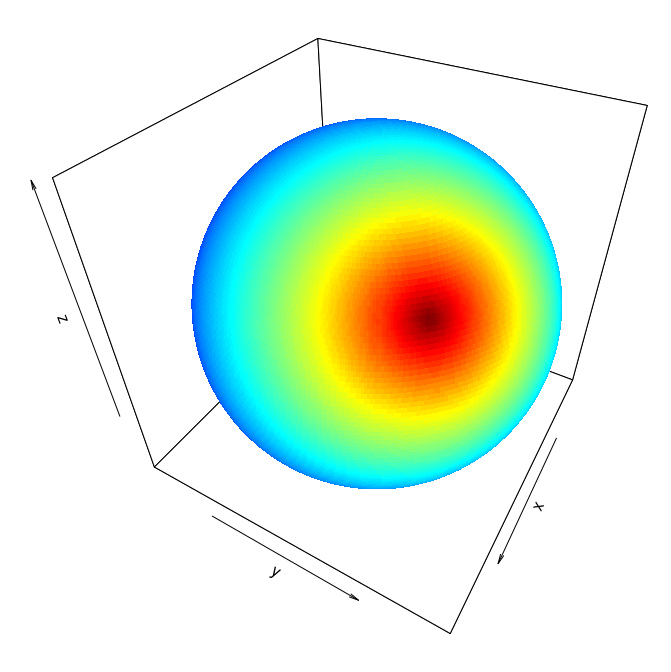
\includegraphics[width=\textwidth]{figures/density_case2.png}
		\caption{$\sigma=1$}
	\end{subfigure}
	\hfill
	\begin{subfigure}[b]{0.3\textwidth}
		\centering
		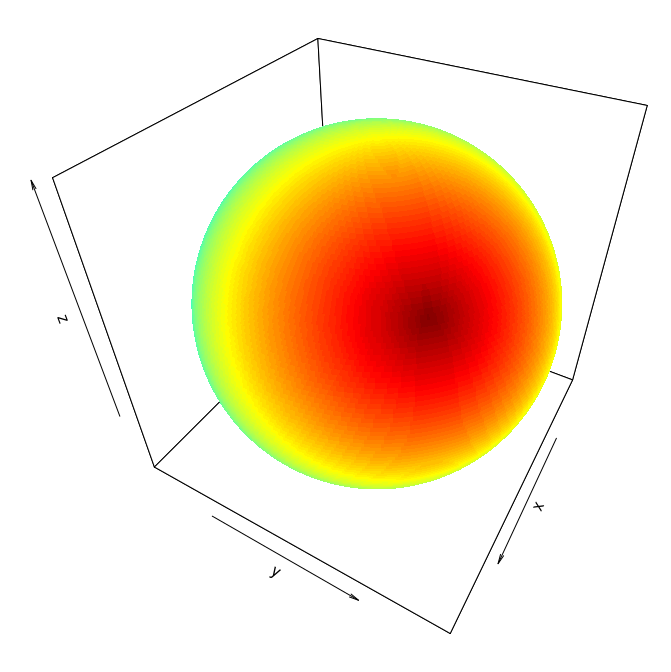
\includegraphics[width=\textwidth]{figures/density_case3.png}
		\caption{$\sigma=5$}
	\end{subfigure}
	\caption{Densities of the SL distribution on $\bbS^2$ with different values of the scale parameter $\sigma$ with $\bfmu = (1,1,1)/\sqrt{3}$. For each plot, regions that are colored in  {\color{red} \bf red} indicate higher densities compared to the area colored as {\color{blue}\bf blue}.}
	\label{fig:three_densities}
\end{figure}

\begin{proposition}\label{theory_proposition} The normalizing constant \eqref{eq:normalizing_constant_full} can be written as a univariate integral as
	\begin{equation}\label{eq:normalizing_constant_simplified}
	C_p (\bfmu, \sigma) = A_{p-1} \int_{r=0}^\pi \exp \left( -\frac{r}{\sigma}\right) \sin^{p-1} (r)dr,
	\end{equation}
	where $A_{p-1} = 2\pi^{p/2} / \Gamma(p/2)$ is the hypervolume or surface area of $\bbS^{p-1}$ and $\Gamma(\cdot)$ is the standard Gamma function. 
\end{proposition}
\begin{proof}[\textbf{\upshape Proof:}]
	On a complete Riemannian manifold, one can characterize the geodesic distance in terms of logarithmic maps and Riemannian metric as $d^2(\bfx, \bfmu) = g_{\bfmu} (\Log_{\bfmu} (\bfx), \Log_{\bfmu} (\bfx))$, which is equivalent to $\Log_{\bfmu} (\bfx)^\top \Log_{\bfmu} (\bfx)$ on $\bbS^p$ with a canonical metric. By a change of variable $\bfu = \Log_{\bfmu} (\bfx)$, a corresponding Jacobian determinant $|\mathbf{J}| = (\sin \|\bfu\| / \|\bfu\|)^{p-1}$ is obtained so that
	\begin{eqnarray}
	C_p (\bfmu, \sigma) &=& \int_{\bbS^p}  \exp \left( -\frac{d(\bfx, \bfmu)}{\sigma} \right) d\bfx =  \int_{\bbS^p}  \exp \left( -\frac{\|\bfu\|}{\sigma}\right) d\bfx \nonumber \\  &=& \int_{\|\bfu \| < \pi} \exp \left( -\frac{\|\bfu\|}{\sigma}\right) \left(\frac{\sin \|\bfu \|}{\|\bfu\|}\right)^{p-1} d\bfu. \label{eq:sub_eqnarray}
	\end{eqnarray}
	We can express the above using spherical coordinate system,
	\begin{eqnarray}
	\eqref{eq:sub_eqnarray} &=& \int_{r=0}^\pi \int_{\varphi_1=0}^\pi \cdots \int_{\varphi_{p-2}=0}^\pi \int_{\varphi_{p-1}=0}^{2\pi} \exp \left(-\frac{r}{\sigma}\right) \left(\frac{\sin r}{r}\right)^{p-1} r^{p-1} \sin^{p-2} (\varphi_1)  \cdots \sin (\varphi_{p-2}) dr d\varphi_1 \cdots d\varphi_{p-1} \nonumber \\
	&=& \int_{\varphi_1=0}^\pi \cdots \int_{\varphi_{p-2}=0}^\pi \int_{\varphi_{p-1}=0}^{2\pi}\sin^{p-2} (\varphi_1)  \cdots \sin (\varphi_{p-2})  d\varphi_1 \cdots d\varphi_{p-1}		 \cdot 
	\int_{r=0}^\pi \exp \left(-\frac{r}{\sigma}\right) \sin^{p-1}(r)dr,\label{eq:sub_surface}
	\end{eqnarray}
	where the first term with nested integrals in \eqref{eq:sub_surface} reduces to the hypervolume $A_{p-1}$ of $\bbS^{p-1}$. 
\end{proof}

Proposition \ref{theory_proposition} does not only lower computational complexity to evaluate the normalizing constant, but also implies that it does not depend on the choice of $\bfmu$. In what follows, we will denote the normalizing constant of the SL distribution as $C_p (\sigma)$ to emphasize its independence on a choice of location $\bfmu$. 


\subsection{Sampling}

It is often of fundamental interest to draw random samples for a given probability distribution. We start by employing a standard rejection sampling technique for its ease of use and efficiency \cite{bishop_2006_PatternRecognitionMachine}. We take the SN distribution as a  proposal density for the rejection sampler whose sampling strategy was well studied in \cite{hauberg_2018_DirectionalStatisticsSpherical}. For a SL distribution with parameters $(\bfmu, \sigma) \in \bbS^p \times \bbRpos$, setting a SN concentration parameter as $\lambda = 1/\sigma$ with the same location $\bfmu$ reduces to a simple rule of acceptance-rejection, which is summarized in Algorithm \ref{code:algorithm_sampling}. Technical details regarding the sampling scheme is described in Appendix.


\begin{algorithm}[t]
	\caption{Rejection Sampling from the SL distribution}
	\label{code:algorithm_sampling}
	\begin{algorithmic}
		\REQUIRE parameters $\bfmu, \sigma$.
		\ENSURE a random sample $\bfx$.
		\STATE Set $\lambda = 1/\sigma$.
		\REPEAT 
		\STATE $u \sim \text{Uniform}(0,1)$.
		\STATE $\bfy \sim \fSN(\bfy~|~\bfmu, \lambda)$.
		\STATE $r \leftarrow d(\bfmu, \bfy)$.
		\STATE $\tau \leftarrow \exp( (r^2-2r-\pi^2+2\pi)  / 2\sigma)$.
		\UNTIL $u \leq \tau$.
		\STATE  Take $\bfx \leftarrow \bfy$.
	\end{algorithmic}
\end{algorithm}

While the rejection sampler is a convenient choice to sample from the SL distribution, one drawback is that the efficiency deteriorates when $\sigma \approx 0$. Recall that the distance is upper bounded by $\pi$ for any two points on the unit hypersphere. When a draw $\bfy$ from a corresponding SN distribution is given, the acceptance threshold $\tau$ is defined as 
\begin{equation*}
\tau = \exp\left( \frac{d^2(\bfmu,\bfy)-2d(\bfmu,\bfy) - \pi^2+2\pi}{2\sigma}\right) = \exp\left(\frac{(d(\bfmu,\bfy)-1)^2 - (\pi-1)^2}{2\sigma}\right),
\end{equation*}
where the numerator within an exponential function is always smaller than or equal to 0. It is trivial to observe that $\tau \rightarrow 1$ as $\sigma \rightarrow \infty$, implying that the rejection sampler almost always accepts a new sample for larger values of a scale parameter $\sigma$. On the other hand, when $\sigma \rightarrow 0$, the threshold converges to 0 in that the sampler requires a tremendously larger number of repeated sampling from its proposal distribution. Hence, it is suggested to use other Markov chain Monte Carlo methods such as the Metropolis-Hastings (MH) algorithm \cite{metropolis_1953_EquationStateCalculations, hastings_1970_MonteCarloSampling} in the regime of small $\sigma$ values. In our numerical experiments, we used the MH sampler where a sequence of samples is generated from a Gaussian distribution on the tangent space at an iterate. 


\subsection{Maximum likelihood estimation}

We now consider the task of maximum likelihood estimation for parameters of the SL distribution. Let $ \bfx_1, \ldots, \bfx_N \in \bbS^p$ be an i.i.d sample from the SL distribution with two parameters,  location $\bfmu$ and scale $\sigma$. The maximum likelihood estimates $(\mleloc, \mlescale) \in \bbS^p \times \bbRpos$ are maximizers of the following log-likelihood function,
\begin{equation}\label{def:log_likelihood}
\begin{split}
L(\bfmu, \sigma) &= \sum_{n=1}^N  \log \left\lbrace \frac{1}{C_p(\sigma)} \exp \left(-\frac{d(\bfx_n,\bfmu)}{\sigma}\right)\right\rbrace\\ 
&= -\frac{1}{\sigma }\sum_{n=1}^N d(\bfx_n, \bfmu) - N \log C_p (\sigma).
\end{split}
\end{equation}
One can observe that \eqref{def:log_likelihood} does not admit closed-form formulae of its maximizers because of the nonlinear terms, engendering the need to employ computational approach for parameter estimation, which will be discussed in the next section.

A closer look at \eqref{def:log_likelihood} allows us to easily recognize that the constrained maximization with respect to $\bfmu$ is independent on the scale parameter since
\begin{equation}\label{eq:mle_location}
\mleloc = \underset{\bfmu \in \bbS^p}{\argmax} -\frac{1}{\sigma}\sum_{n=1}^N d(\bfx_n, \bfmu) = \underset{\bfmu \in \bbS^p}{\argmin} \sum_{n=1}^N d(\bfx_n, \bfmu).
\end{equation}
In the literature of manifold-valued statistics, the objective to minimize sum of distances has been known as the \Frechet or geometric median problem \cite{fletcher_2009_GeometricMedianRiemannian, arnaudon_2013_MediansMeansRiemannian}. Once $\mleloc$ is obtained, solving for $\sigma$ is merely a univariate minimization problem as follows,
\begin{equation}\label{eq:mle_scale}
\mlescale = \underset{\sigma\in\bbRpos}{\argmax} -\frac{1}{\sigma} \sum_{n=1}^N d(\bfx_n, \mleloc) - N \log C_p (\sigma) = \underset{\sigma\in\bbRpos}{\argmin~} \frac{S}{\sigma} + \log C_p(\sigma),
\end{equation}
for a fixed constant $S = \sum_{n=1}^N d(\bfx_n, \mleloc)/N$. We show existence and uniqueness of maximum likelihood estimates in the following theorem under some conditions.

\begin{theorem}\label{theory_theorem}
	Let $\bfx_1, \ldots, \bfx_N$ be an i.i.d sample on a $p$-dimensional unit hypersphere $\bbS^p$. If the sample is contained in an open geodesic ball $B(\bfx, \pi/4)$ for some $\bfx \in \bbS^p$ and not totally contained in any geodesic, maximum likelihood estimates $(\mleloc, \mlescale)$ uniquely exist. 
\end{theorem}
\begin{proof}[\textbf{\upshape Proof:}] We first use the characterization of maximum likelihood estimate for location parameter of the SL distribution as the \Frechet median. Conditions for existence and uniqueness have been extensively studied on a general Riemannian manifold $\calM$ \cite{yang_2010_RiemannianMedianIts, arnaudon_2013_MediansMeansRiemannian}, whose statements are phrased as follows for completeness. Let $\bar{B}(\bfx, \rho)$ and $\Delta$ denote a closed geodesic ball of radius $\rho$ centered at $\bfx \in \calM$ and an upper bound of sectional curvatures in $\bar{B}(\bfx, \rho)$, respectively. Theorem 3.1 of \cite{yang_2010_RiemannianMedianIts} states that if a sample is not totally contained in any geodesic and the radius satisfies
	\begin{equation*}
	\rho < \min \left\lbrace \frac{\pi}{4\sqrt{\Delta}}, \frac{\textrm{inj} (\bar{B}(\bfx, \rho))}{2} \right\rbrace,
	\end{equation*}
	the \Frechet median exists and is unique because the objective function becomes strictly convex under the stated conditions. The unit hypersphere has a constant sectional curvature so that $\Delta = 1$ and an injectivity radius is $\pi$ at all points. Therefore, the maximal convexity radius $\rho$ is $\min \lbrace  \pi/4, \pi/2 \rbrace = \pi/4$ on $\bbS^p$. On top of a support condition of a random sample being not totally contained in any geodesic, this establishes the existence and uniqueness of $\mleloc$. 
	
	We now turn to examine the scale parameter. Let $g(\sigma) = S/\sigma + \log C_p (\sigma)$ with a known constant $S \in [0, \pi]$ as the geodesic distance between any two points on the sphere is bounded above by the injectivity radius $\pi$. It needs to be shown that $g(\sigma)$ admits a unique critical point.	The first-order condition $g'(\sigma) = 0$ is equivalent to whether $-S C_p(\sigma) + \sigma^2 C_p'(\sigma)=0$. Hence, it is sufficient to show if $G(S) = -S C_p(\sigma) + \sigma^2 C_p'(\sigma)$ has a unique zero in $(0,\pi)$ for any choice of $\sigma$. This implies a bijection between $S$ and $\sigma$, establishing the existence and uniqueness for a critical point of $g(\sigma)$ equivalently. 
	
	First, it is trivial that $G(S)$ is a continuous function since every term consists of smooth, bounded functions on a finite interval. Second, we have $G(0) > 0$ as
	\begin{eqnarray*}
		G(0) &=& \sigma^2 C_p'(\sigma) \\
		&=& \sigma^2 \cdot  A_{p-1} \int_{r=0}^\pi \frac{r}{\sigma^2} \exp \left( -\frac{r}{\sigma}\right) \sin^{p-1}(r)dr \\
		&=& A_{p-1} \int_{r=0}^\pi r \exp  \left( -\frac{r}{\sigma}\right) \sin^{p-1}(r)dr,
	\end{eqnarray*}
	where all terms in the integrand are positive on $(0,\pi)$. On the other end, $G(\pi) < 0$ since  
	\begin{eqnarray*}
		G(\pi) &=& -\pi C_p(\sigma) + \sigma^2 C_p'(\sigma)\\
		&=& A_{p-1} \left\lbrace  -\pi \int_{r=0}^\pi \exp \left(-\frac{r}{\sigma}\right)\sin^{p-1}(r)dr + \sigma^2 \int_{r=0}^\pi \frac{r}{\sigma^2}\exp \left( -\frac{r}{\sigma}\right) \sin^{p-1}(r)dr \right\rbrace \\
		&=& A_{p-1} \int_{r=0}^\pi (-\pi + r) \exp \left( -\frac{r}{\sigma}\right) \sin^{p-1}(r)dr ,
	\end{eqnarray*}
	and $-\pi+r < 0$ while the other terms in the integrand are strictly positive except for a measure zero set. Lastly, $G(S)$ is a monotonically decreasing function. Take $S' \in (0,\pi)$ such that $S < S'$, then 
	\begin{eqnarray*}
		G(S')-G(S) &=& -S' C_p (\sigma) + \sigma^2 C_p'(\sigma) - ( -S C_p (\sigma) + \sigma^2 C_p'(\sigma) ) \\
		&=& (S - S') C_p(\sigma) < 0.
	\end{eqnarray*}
	By the intermediate value theorem and monotonicity, $G(S)$ has a unique zero in $(0,\pi)$ and so does $g'(\sigma)$, which completes the proof. 
\end{proof}


%%%%%%%%%%%%%%%%%%%%%%%%%%%%%%%%%%%%%%%%%%%%%%%%%%%%%%%%%%%%%%%%%%%%%%%%%%%%%%%%%%%%%%%%%%%%%%%%%%%%%%
\section{Parameter estimation}\label{sec4:parameter}

It was observed in the previous section that maximum likelihood estimation for parameters of the SL distribution can be decomposed into two components in a sequential manner to solve the standard \Frechet median problem for the location parameter $\bfmu \in \bbS^p$ and a univariate optimization problem for the scale parameter $\sigma \in \bbRpos$. Throughout this section, we consider a more general scenario where each $\bfx_n$ is weighted by a non-negative constant $w_n > 0$ that sums to 1, i.e., $\sum_{n=1}^N w_n = 1$, and present adapted algorithms to the context. This is because it not only reduces to the maximum likelihood estimation when all weights are set to be equal, but also this formulation provides useful apparatus for model-based clustering in the following section. 

\subsection{Estimation of the location}

Given a random sample $\bfx_1, \ldots, \bfx_N \in \bbS^p$ and corresponding non-negative weights $w_1, \ldots, w_N$, the weighted \Frechet median problem is written as 
\begin{equation}\label{eq:objective_location}
\underset{\bfmu\in\bbS^p}{\min~} F(\bfmu) = \underset{\bfmu\in\bbS^p}{\min~} \sum_{n=1}^N w_n d(\bfx_n, \bfmu),
\end{equation}
where $\mleloc$ is a solution to the special case of \eqref{eq:objective_location} if all weights $w_n$'s are equal such as $w_1 = \cdots = w_N = 1/N$. 

We employ a geometric variant of the Weiszfeld algorithm \cite{fletcher_2009_GeometricMedianRiemannian}, whose standard version has long been known in the Euclidean regime \cite{weiszfeld_1937_PointPourLequel}. In general, the Weiszfeld algorithm follows a descent path, making it to belong to a class of gradient descent methods. At each iteration, an iterate is updated by varying amount of step size determined by a fixed rule. This removes potentially large computational burden to tune step sizes by line search at each iteration.

Now a geometric Weiszfeld algorithm is described for the weighted \Frechet median problem, which is summarized in Algorithm \ref{code:algorithm_location}. Roughly speaking,  the gradient $\textrm{grad} F\vert_{\bfx}$ of a scalar-valued function $F$ on a manifold $\calM$ is defined as a vector field, meaning that it takes a value as a tangent vector in $T_{\bfx} \calM$. Once an update is done in the gradient direction, an additional step is necessary   to push an iterate onto the manifold itself \cite{absil_2008_OptimizationAlgorithmsMatrix}. Using the variation of energy, it can be readily shown that $\text{grad}~ d(\bfmu, \bfx)\vert_{\bfmu} = -\Log_{\bfmu} (\bfx) / d(\bfmu, \bfx)$, leading to define a gradient of \eqref{eq:objective_location} at iteration $t$ as
\begin{equation*}
\textrm{grad}~ F\vert_{\bfmu^{(t)}} = -\sum_{n=1}^N \frac{w_n}{d(\bfx_n, \bfmu^{(t)})} \Log_{\bfmu^{(t)}} (\bfx_n) =- \sum_{n=1}^N w_n^{(t)} \Log_{\bfmu^{(t)}} (\bfx_n).
\end{equation*}
The geometric Weiszfeld algorithm updates an iterate by 
\begin{eqnarray}
\bfmu^{(t+1)} &=& \Exp_{\bfmu^{(t)}} \left( -\alpha^{(t)}  \textrm{grad}~ F\vert_{\bfmu^{(t)}} \right) \nonumber \\ 
&=& \Exp_{\bfmu^{(t)}} \left(
\frac{\sum_{n=1}^N w_n^{(t)} \Log_{\bfmu^{(t)}}(\bfx_n)}{\sum_{n=1}^N w_n^{(t)}}
\right),\label{eq:update_location_weiszfeld}
\end{eqnarray}
with an automatically-determined step size $\alpha^{(t)}=1/\sum_{n=1}^N w_n^{(t)}$. In our context, exponential and logarithmic maps are computed using the formula introduced in \eqref{eq:map_exponential} and \eqref{eq:map_logarithmic}.


\begin{algorithm}[t]
	\caption{Weighted \Frechet median computation}
	\label{code:algorithm_location}
	\begin{algorithmic}
		\REQUIRE a random sample $\bfx_1, \ldots, \bfx_N \in \bbS^p$,  weights $w_1, \ldots, w_N$, stopping criterion $\epsilon$.
		\ENSURE $\hat{\bfmu} = \argmin F(\bfmu)$ where $F(\bfmu) =  \sum_{n=1}^N w_n  d (\bfx_n, \bfmu)$ for $\bfmu \in \bbS^p$. 
		\STATE Initialize $\bfmu^{(0)} = \sum_{n=1}^N w_n \bfx_n / \| \sum_{n=1}^N w_n \bfx_n \|$.
		\REPEAT 
		\STATE Compute scaled weights $w_n^{(t)} = w_n / d(\bfmu^{(t)}, \bfx_n)$ for $n\in\lbrace 1,\ldots, N\rbrace$. 
		\STATE Update an iterate $\bfmu^{(t+1)}$ by \eqref{eq:update_location_weiszfeld}.
		\IF{$\bfmu^{(t+1)}$ equals to one of $\bfx_1, \ldots, \bfx_N$}
		\STATE stop the algorithm.
		\ENDIF
		\UNTIL $d(\bfmu^{(t)}, \bfmu^{(t+1)})$ or  $\| \bfmu^{(t)} - \bfmu^{(t+1)} \|$ is smaller than $\epsilon$.
		\STATE  Take $\hat{\bfmu} = \bfmu^{(t+1)}$.
	\end{algorithmic}
\end{algorithm}

We close by discussing some technical components of Algorithm \ref{code:algorithm_location}. At the initial stage, a starting point is taken as $\bfmu^{(0)} = \sum_{n=1}^N w_n \bfx_n / \| \sum_{n=1}^N w_n \bfx_n\|$. This quantity is equivalent to an extrinsic mean of a random sample \cite{bhattacharya_2012_NonparametricInferenceManifolds}, which is also a maximum likelihood estimate of a location parameter from the vMF distribution. When a random sample is adequately concentrated as stated in Theorem \ref{theory_theorem}, an extrinsic mean can be a reasonable choice as it is contained in a convex geodesic ball. Moreover, it only requires elementary arithmetic operations without any need for expensive computational routines to be performed. Second, it is standard to halt iterations when an iterate belongs to a set of given observations. A direct reason is that a scaled weight cannot be evaluated if $d(\bfmu^{(t+1)}, \bfx_n)=0$ for any $n$ at the next iteration. Ad hoc remedies include to re-initialize an algorithm, remove a matching point from computation in the specific step, or pad 0 with a very small positive number, all of which we do not consider in this paper. Lastly, the stopping criterion by sufficiently small incremental geodesic change $d(\bfmu^{(t)}, \bfmu^{(t+1)})$ is based from a fact that the unit hypersphere is a complete Riemannian manifold, which guarantees to measure convergence of a sequence in the sense of Cauchy. One may also choose to use the $\ell_2$ norm-based stopping rule since intrinsic and extrinsic distances converge as two points get sufficiently close on a complete manifold embedded in some Euclidean space. 
\subsection{Estimation of the scale}

Maximum likelihood estimation for the scale parameter $\sigma$ of the SL distribution is merely a univariate minimization of the following objective function
\begin{equation*}
g(\sigma) = \frac{S}{\sigma} + \log C_p (\sigma),
\end{equation*} 
given a fixed constant $S = \sum_{n=1}^N d (\bfx_n, \mleloc) / N$. According to the Theorem \ref{theory_theorem}, the cost function admits a unique critical point. Hence, it can be cast as a root-finding problem of $g'(\sigma) = 0$. 

In order to estimate the scale parameter, we use the Newton-Raphson method \cite{ypma_1995_HistoricalDevelopmentNewton, burden_2016_NumericalAnalysis} for root-finding. When a univariate  function of interest $f:\bbR \rightarrow \bbR$ has continuous derivatives up to order 0, the Newton-Raphson algorithm solves $f(x) = 0$ by updating an iterate as $x^{(t+1)} = x^{{(t)}} - {f(x^{(t)})}/{f'(x^{(t)})}$ with an initial point $x^{(0)}$. By setting $f = g'$, we can easily derive the updating rule to solve $g'(\sigma) = 0$ by  $\sigma^{(t+1)} = \sigma^{(t)} - {g'(\sigma^{(t)})}/{g''(\sigma^{(t)})}$. Define the quantities
\begin{eqnarray*}
	I_0 (\sigma) &=& \int_{r=0}^\pi \exp \left( -\frac{r}{\sigma}\right) \sin^{p-1}(r)dr, \\
	I_1 (\sigma) &=& \int_{r=0}^\pi \frac{r}{\sigma^2} \exp \left( -\frac{r}{\sigma}\right) \sin^{p-1}(r)dr, \\
	I_2 (\sigma) &=& \int_{r=0}^\pi \left(\frac{r^2}{\sigma^4} - \frac{2r}{\sigma^3}\right) \exp \left( -\frac{r}{\sigma}\right) \sin^{p-1}(r)dr,
\end{eqnarray*}
which are integrals related to the normalizing constant and its derivatives. By re-writing derivatives of $g$ with respect to the above integrals, we can simplify the Newton-Raphson update at iteration $t$ as
\begin{eqnarray}
\sigma^{(t+1)} = \sigma^{(t)} - 
\left(
-\frac{S}{(\sigma^{(t)})^2} + \frac{I_1 (\sigma^{(t)})}{I_0 (\sigma^{(t)})} 
\right) \Bigg/ \left(
\frac{2S}{(\sigma^{(t)})^3} + \frac{I_0 (\sigma^{(t)}) I_2 (\sigma^{(t)}) - (I_1 (\sigma^{(t)}))^2}{(I_0 (\sigma^{(t)}))^2}
\right).\label{eq:update_scale_newton_exact}
\end{eqnarray}


When $\sigma$ is close to zero, evaluation of $I_1(\sigma)$ and $I_2 (\sigma)$ may suffer from numerical instability due to presence of $\sigma$ in rational terms, while $I_0 (\sigma)$ is more robust to obtain from a computational point of view. As a result, an alternative to \eqref{eq:update_scale_newton_exact} is considered by computing derivatives with the centered finite difference schemes as follows,
\begin{eqnarray*}
	g'(\sigma) &\approx& \frac{g(\sigma+h) - g(\sigma-h)}{2h}, \\
	g''(\sigma) &\approx& \frac{g(\sigma+h) - 2g(\sigma) + g(\sigma-h)}{h^2},
\end{eqnarray*}
for a sufficiently small step-size $h>0$. By plugging in the approximate derivatives, we get an updating rule
\begin{eqnarray}
\sigma^{(t+1)} = \sigma^{(t)} - \frac{h}{2} \cdot \frac{g(\sigma^{(t)}+h) - g(\sigma^{(t)}-h)}{g(\sigma^{(t)}+h) - 2g(\sigma^{(t)}) + g(\sigma^{(t)}-h)}
.\label{eq:update_scale_newton_approx}	
\end{eqnarray}


We note that an approximate updating rule \eqref{eq:update_scale_newton_approx} has equivalent computational complexity to that of \eqref{eq:update_scale_newton_exact} as both integrate one-dimensional smooth functions three times per  iteration.% \textbf{NEED TO WRITE MORE ON THINGS LIKE CHOICE OF H.}






\begin{algorithm}[t]
	\caption{Maximum likelihood estimation of the scale parameter}
	\label{code:algorithm_scale}
	\begin{algorithmic}
		\REQUIRE a random sample $\bfx_1, \ldots, \bfx_N \in \bbS^p$, a constant $S$, stopping criterion $\epsilon$.
		\ENSURE $\mlescale = \argmin g(\sigma)$ where $g(\sigma) = S/\sigma + \log C_p (\sigma)$ for $\sigma \in \bbRpos$. 
		\STATE Initialize $\sigma^{(0)}$. 
		\REPEAT 
		\STATE Update an iterate $\sigma^{(t+1)}$ by either \eqref{eq:update_scale_newton_exact} or \eqref{eq:update_scale_newton_approx}.
		\UNTIL $|\sigma^{(t)} - \sigma^{(t+1)}|<\epsilon$.
		\STATE  Take $\mlescale = \sigma^{(t+1)}$.
	\end{algorithmic}
\end{algorithm}




%%%%%%%%%%%%%%%%%%%%%%%%%%%%%%%%%%%%%%%%%%%%%%%%%%%%%%%%%%%%%%%%%%%%%%%%%%%%%%%%%%%%%%%%%%%%%%%%%%%%%%
\section{Application to clustering}\label{sec5:clustering}

One of the direct applications for parameter estimation of the SL distribution is probabilistic clustering of sphere-valued data using finite mixture models \cite{mclachlan_2019_FiniteMixtureModels}. The density of a finite mixture model of $K$ SL components is 
\begin{eqnarray*}
	h(\bfx | \mathbf{\Theta}) = \sum_{k=1}^K \pi_k \fSL(\bfx~|~\bfmu_k, \sigma_k),
\end{eqnarray*}
for component weights $\pi_k,~k\in\lbrace 1,\ldots, K\rbrace$ such that $\sum_{k=1}^K \pi_k = 1$ and parameters $\bfTheta = \lbrace \pi_k, \bfmu_k, \sigma_k\rbrace_{k=1}^K$. We follow a standard approach to maximize log-likelihood given a random sample $\bfX = \lbrace \bfx_1, \ldots, \bfx_N\rbrace \subset \bbS^p$ by introducing latent variables for class membership and applying  Expectation-Maximization (EM) algorithm \cite{dempster_1977_MaximumLikelihoodIncomplete}. We refer interested readers to \cite{bishop_2006_PatternRecognitionMachine} for thorough description of the technique. To briefly introduce, denote a binary matrix of latent class memberships as $\bfZ \in \lbrace 0, 1\rbrace^{N\times K}$ such that every row of $\bfZ$ contains only one non-zero element and the joint distribution of $\bfX$ and $\bfZ$ as
\begin{eqnarray*}
	\rmP(\bfX,\bfZ~|~\bfTheta) = \prod_{n=1}^N \prod_{k=1}^K \left( \pi_k \fSL(\bfx_n~|~\bfmu_k, \sigma_k)\right)^{z_{nk}}.
\end{eqnarray*}
The EM algorithm alternates E- and M-steps. At iteration $t$, the E-step evaluates posterior distribution of the latent variable  $\rmP(\bfZ~|~\bfX,\bfTheta^{(t)})$ to compute the complete-data log-likelihood
\begin{eqnarray*}
	Q(\bfTheta~|~\bfTheta^{(t)}) = \sum_{\bfZ} \rmP(\bfZ~|~\bfX, \bfTheta^{(t)}) \log \rmP (\bfX, \bfZ~|~\bfTheta) = \rmE_{\bfZ|\bfX, \bfTheta^{(t)}} \lbrack \log \rmP(\bfX, \bfZ~|~\bfTheta) \rbrack,
\end{eqnarray*}
and the M-step updates all parameters $\bfTheta^{(t+1)}$ by maximizing $Q(\bfTheta~|~\bfTheta^{(t)})$. 

We now elaborate on explicit expressions for updating parameters in a finite mixture of SL distributions under the standard EM framework at iteration $t$. The E-step starts by evaluating posterior of the latent variables, which first reduces to evaluating $\rmE[z_{nk}]$ as follows,
\begin{eqnarray}
\gamma_{nk} := \rmE[z_{nk}] = \frac{\pi_k^{(t)} \fSL(\bfx_n~|~\bfmu_k^{(t)}, \sigma_k^{(t)})}{\sum_{j=1}^K \pi_j^{(t)} \fSL(\bfx_n~|~\bfmu_j^{(t)}, \sigma_j^{(t)})},
\end{eqnarray}
for $(n,k) \in \lbrace 1,\ldots, N\rbrace \times \lbrace 1,\ldots, K\rbrace$. Let $\bfGamma := \gamma_{nk} \in [0,1]^{N\times K}$ denote a matrix of posterior for the latent variables known as soft clustering or membership matrix. An $(n,k)$-th entry of $\bfGamma$ encodes information on how likely an observation $\bfx_n$ belongs to the $k$-th cluster. Given the evaluations, the complete-data log-likelihood can be written as
\begin{eqnarray*}
	Q(\bfTheta~|~\bfTheta^{(t)}) = \sum_{n=1}^N \sum_{k=1}^K \gamma_{nk} \left\lbrace 
	\log \pi_k + \log \fSL (\bfx_n~|~\bfmu_k, \sigma_k)
	\right\rbrace,
\end{eqnarray*}
which is an objective function for maximization in the M-step. For each component $k\in\lbrace 1,\ldots,K\rbrace$,  weight and location parameters are updated as follows,
\begin{eqnarray}
\pi_k^{(t+1)} &=& \frac{\sum_{n=1}^N \gamma_{nk}}{N},\nonumber\\
\bfmu_k^{(t+1)} &=& \underset{\bfmu \in \bbS^p}{\argmin~} \sum_{n=1}^N \gamma_{nk} \cdot d(\bfx_n, \bfmu), \label{eq:EM_location}
\end{eqnarray}
where \eqref{eq:EM_location} is a weighted \Frechet median problem that can be solved using Algorithm \ref{code:algorithm_location} with $w_i = \gamma_{ik},~i\in\lbrace 1,\ldots, N\rbrace$. Lastly, scale parameters are solutions of the following problems,
\begin{eqnarray}\label{eq:EM_scale_hetero}
\sigma_k^{(t+1)} = \underset{\sigma \in \bbRpos}{\argmin~} \left(\frac{\sum_{n=1}^N \gamma_{nk} \cdot d(\bfx_n, \bfmu_k^{(t+1)})}{\sum_{n=1}^N \gamma_{nk}}\right) \cdot \frac{1}{\sigma} + \log C_p (\sigma),
\end{eqnarray}
which can be solved by Algorithm \ref{code:algorithm_scale}. 



We now turn to discuss some aspects of the model and EM algorithm. First, one way to regularize varying scales across multiple components is to use a common scale parameter rather than component-specific values, i.e., $\sigma = \sigma_1 = \cdots = \sigma_K$. In this setting, the model is called homogeneous and a common scale parameter is updated by
\begin{eqnarray}\label{eq:EM_scale_homo}
\sigma^{(t+1)} = \underset{\sigma \in \bbRpos}{\argmin~} \left(\frac{\sum_{n=1}^N \sum_{k=1}^K \gamma_{nk} \cdot d(\bfx_n, \bfmu_k^{(t+1)})}{\sum_{n=1}^N \sum_{k=1}^K \gamma_{nk}}\right) \cdot \frac{1}{\sigma} + \log C_p (\sigma).
\end{eqnarray}

Second, computational cost of the algorithm becomes prohibitive when the sample size $N$ grows. Especially, updating location parameters via \eqref{eq:EM_location} is problematic since the membership matrix $\bfGamma$ is highly likely to be dense and a weighted \Frechet median over a large number of observations needs to be computed. We present two popular heuristics to reduce the sample size - hard and stochastic assignments - that directly manipulate $\bfGamma$ so that the pertained computation is limited to a smaller subset of the sample. Denote the $n$-th row of $\bfGamma$ as $\bfGamma_n$ and $\textsf{sample}(\mathbf{v}_z, \textrm{probability}=\mathbf{p}_z)$ is a sampling procedure to randomly draw an element from a vector  $\mathbf{v}_z$ with probability $\mathbf{p}_z$.  Two  assignments are done as follows,
\begin{eqnarray}
\textsf{hard}(\gamma_{nk}) &=& \begin{cases}
1, &\textrm{if $k$ is maximal index of $\bfGamma_n$,}\\0, &\textrm{otherwise}.
\end{cases} \label{eq:heuristic_hard}	\\
\textsf{stochastic}(\gamma_{nk}) &=& \begin{cases}
1, &\textrm{if $k=\textsf{sample}(1:K, ~\textrm{probability}=\bfGamma_n)$},\\
0, &\textrm{otherwise}. \label{eq:heuristic_stochastic}
\end{cases}
\end{eqnarray}
The hard assignment is equivalent to predict discrete-valued label for an observation, while the stochastic assignment performs the same task in a probabilistic manner. Given a large sample, these sparsification strategies help to reduce execution time and space complexity in updating both location and scale parameters. We note that the hard assignment is optimal in the sense that a lower bound of the incomplete-data log-likelihood is maximized \cite{banerjee_2005_ClusteringUnitHypersphere}. 


Third, we describe some practical details from an implementation side. We initialize the algorithm using partition structure obtained from $k$-means clustering \cite{macqueen_1967_MethodsClassificationAnalysis}. This is because most computing platforms are equipped with efficient, robust implementations of the algorithm. Besides, a large amount of geometric information is preserved by an equivariant embedding \cite{bhattacharya_2012_NonparametricInferenceManifolds}, which is the identity map on $\bbS^p$, in that this approach preserves certain degree of geometric information. Another practical issue is to determine convergence of the algorithm. It is natural to terminate iterations if log-likelihood stops to increase. From a computational perspective, however, the log-likelihood is not an appealing option since computing the quantity requires density evaluation with updated parameters at each iteration while no intermediate quantities may be used. Hence, we suggest to use incremental change in a soft clustering matrix $\|\bfGamma^{(t+1)} - \bfGamma^{(t)}\|$ as a quantity to terminate iterations since it implies that clustering results do not evolve and no extra updates are needed.


We close this section by considering a potential variant of our model. The finite mixture model has long been known to be closely related to the $k$-means algorithm, which has been also observed in the context of directional statistics  \cite{dhillon_2001_ConceptDecompositionsLarge, banerjee_2005_ClusteringUnitHypersphere, bishop_2006_PatternRecognitionMachine}. Assuming the homogeneous model of equal scale, an entry of membership matrix $\bfGamma$ is written as 
\begin{eqnarray}
\gamma_{nk} = \frac{\pi_k^{(t)} \fSL(\bfx_n~|~\bfmu_k^{(t)}, \sigma_k^{(t)})}{\sum_{j=1}^K \pi_j^{(t)} \fSL(\bfx_n~|~\bfmu_j^{(t)}, \sigma_j^{(t)})} = 
\frac{\pi_k \exp \left( -{d(\bfx_n, \bfmu_k)}/{\sigma} \right) }{\sum_{j=1}^K \pi_j \exp \left( -{d(\bfx_n, \bfmu_j)}/{\sigma} \right)},
\end{eqnarray}
which quantifies likelihood for the $n$-th observation to belong to the $k$-th component or cluster. Let $k^*$ be an index for $d(\bfx_n, \bfmu_k)$ being the smallest. When $\sigma \rightarrow 0$, the term $d(\bfx_n, \bfmu_{k^*})$ decays at the slowest rate in the denominator than others so that all other $\gamma_{nk}$'s approach to zero. This procedure is identical to how the $k$-medians clustering algorithm updates assignment of each observation. We can validate this reasoning by taking a limit of the complete-data log-likelihood
\begin{eqnarray}
\rmE_{\bfZ|\bfX, \bfTheta} \lbrack \log \rmP(\bfX,\bfZ|\bfTheta) \rbrack  \xrightarrow{\sigma \rightarrow 0} - \sum_{n=1}^N \sum_{k=1}^K \gamma_{nk} d(\bfx_n, \bfmu_k) + \textrm{some constant}.
\end{eqnarray}
Therefore, in the limit sense, maximizing the expected complete-data log-likelihood amounts to minimization of cost function in a generic $k$-medians problem, which has not been popularized in directional statistics up to our knowledge. 









\begin{algorithm}[ht]
	\caption{EM algorithm for the mixture of SL distributions.}
	\label{code:em_splaplace}
	\begin{algorithmic}
		\REQUIRE a random sample $\bfx_1, \ldots, \bfx_N \in \bbS^p$, number of clusters $K$.
		\ENSURE a soft clustering/membership matrix $\bfGamma$.		
		\STATE Initialize $ \bfTheta^{(0)} = \lbrace \pi_k^{(0)}, \bfmu_k^{(0)}, \sigma_k^{(0)}\rbrace_{k=1}^K$.
		\REPEAT 
		\STATE \{E-step\}
		\FOR{$n=1:N$}
		\FOR {$k=1:K$ }
		\STATE $\bfGamma (n,k)= \pi_k^{(t)} \fSL (\bfx_n~\vert~ \bfmu_k^{(t)}, \sigma_k^{(t)})$
		\ENDFOR
		\STATE $\bfGamma(n,:) = \bfGamma(n,:)/ \sum_{k=1}^K \bfGamma(n,k)$
		\ENDFOR 
		\STATE \{Heuristics\}
		\IF {hard assignment}
		\STATE $\bfGamma \leftarrow \textsf{hard}(\bfGamma)$ by \eqref{eq:heuristic_hard}.
		\ELSIF {stochastic assignment}
		\STATE $\bfGamma \leftarrow \textsf{stochastic}(\bfGamma)$ by \eqref{eq:heuristic_stochastic}.
		\ENDIF
		\STATE \{M-step\}
		\FOR{$k=1:K$}
		\STATE $\pi_k^{(t+1)} = \sum_{n=1}^N \gamma_{nk} / N$.
		\STATE $\bfmu_k^{(t+1)} = \underset{\bfmu \in \bbS^p}{\argmin~}  \sum_{n=1}^N \gamma_{nk} \cdot d (\bfx_n, \bfmu)$ by Algorithm \ref{code:algorithm_location}. 
		\ENDFOR
		\IF {homogeneous model}
		\STATE Update $\sigma^{(t+1)}$ using \eqref{eq:EM_scale_homo} by Algorithm \ref{code:algorithm_scale}.
		\ELSE
		\FOR {$k=1:K$}
		\STATE  Update $\sigma_k^{(t+1)}$ using \eqref{eq:EM_scale_hetero} by Algorithm \ref{code:algorithm_scale}. 
		\ENDFOR
		\ENDIF
		\UNTIL convergence.
	\end{algorithmic}
\end{algorithm}




%%%%%%%%%%%%%%%%%%%%%%%%%%%%%%%%%%%%%%%%%%%%%%%%%%%%%%%%%%%%%%%%%%%%%%%%%%%%%%%%%%%%%%%%%%%%%%%%%%%%%%
\section{Experiments}\label{sec6:experiments}

We come to assess how the proposed algorithms perform for the tasks of parameter estimation and model-based clustering. The first experiment is composed of evaluating parameter estimation algorithms with simulated data. Then, we investigate effectiveness of model-based clustering with the finite mixture of SL distributions using simulated and real data examples. 





\subsection{Estimating parameters}

We evaluate performance of the proposed algorithms for maximum likelihood estimation of two parameters. We start by presenting  the simplest case where two fixed parameters $\bfmu_0 \in (1,0,0,0,0,0)^\top \in \bbS^{5}$ and $\sigma_0 = 0.1$ are used to generate random samples of varying size from 25 to $475$. Each setting is run 100 times and empirical distributions of two performance measures, run time and accuracy, are reported. For numerical optimization, the stopping criterion of $\epsilon = 10^{-8}$ was used throughout all computations, which is approximately equal to a square root of the machine epsilon in double precision. 

For the location estimation problem, we compared the geometric Weiszfeld method as shown in Algorithm \ref{code:algorithm_location} and the standard version of Riemannian gradient descent (RGD) algorithm. The latter relies on line search to determine how much an iterate shall proceed along the descent direction. Given a random sample $\bfX = \{\bfx_1, \ldots, \bfx_n\} \subset \bbS^5$ and a maximum likelihood estimate $\hat{\bfmu}_{\mathrm{MLE}}$, accuracy is measured by the geodesic distance $d(\hat{\bfmu}_{\textrm{MLE}}, \bfmu_0) = \cos^{-1}(\langle \hat{\bfmu}_{\textrm{MLE}}, \bfmu_0\rangle)$. Two performance measures under the setting are shown in \figurename \ref{fig:estimation_location}. As the sample size grows, it is seen that better estimates are obtained in both methods at almost parallel levels of accuracy. In terms of computational cost, however, the Weiszfeld algorithm consistently outperforms the RGD and the degree of disparity gets larger along the growing sample size. This is an expected phenomenon in the sense that line search requires repeated evaluation of the cost functional while the Weiszfeld algorithm requires a single evaluation at each iteration. Therefore, the RGD may converge in fewer iterations than the Weiszfeld algorithm at the increased cost of overall computation. 
\begin{figure}[h]
	\centering
	
\includegraphics[width=0.95\linewidth]{figures/estimation_location-eps-converted-to.pdf}
	\caption{Empirical distribution of performance measures, (a) accuracy and (b) elapsed time, for the location estimation problem. At each run, a random sample from the SL distribution of parameters $\bfmu_0 = (1,0,0,0,0,0)^\top, \sigma_0 = 0.1$ was drawn and the procedure was repeated 100 times. }
	\label{fig:estimation_location}
\end{figure}

Similarly, we compared performance of the proposed Newton's methods against two univariate optimization routines that do not require derivative information. Our first choice is a default optimization routine in \textsf{R} programming language \cite{rcoreteam_2022_LanguageEnvironmentStatistical} that uses golden-section search with successive parabolic interpolation, which we will denote as \textsf{Roptim}. Another is the differential evolution algorithm for global optimization using a heuristic approach \cite{storn_1997_DifferentialEvolutionSimple} and will be denoted as \textsf{DE}. We derived two updating rules for the Newton's methods using exact integral evaluation and approximation of the derivatives using finite difference, which will be called as \textsf{NewtonE} and \textsf{NewtonA}, respectively. We measured accuracy of the estimate  $\hat{\sigma}_{\textrm{MLE}}$ by relative error $|\hat{\sigma}_{\textrm{MLE}} - \sigma_0|/\sigma_0$. Performance measures for all 4 algorithms under the aforementioned setting are summarized in \figurename \ref{fig:estimation_scale}. The quality of estimation was comparable across all methods, which is not surprising since all algorithms start from an identical location estimate. When it comes to computational efficiency, however, both our proposed algorithms show superior performance to the others.

\begin{figure}[ht]
	\centering
	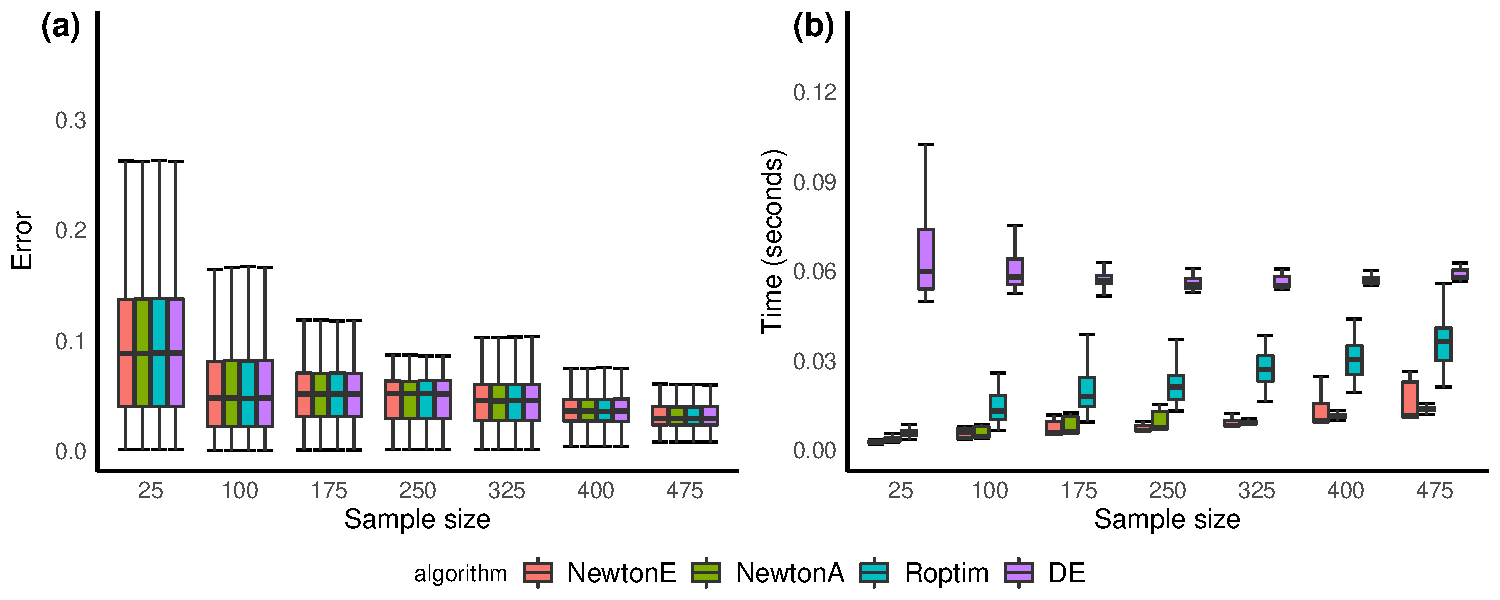
\includegraphics[width=0.95\linewidth]{figures/estimation_scale-eps-converted-to.pdf}
	\caption{Empirical distribution of performance measures, (a) accuracy and (b) elapsed time, for the scale estimation problem. Each run drew a random sample from the SL distribution parametrized by $\bfmu_0 = (1,0,0,0,0,0)^\top, \sigma_0 = 0.1$. The procedure was repeated 100 times. }
	\label{fig:estimation_scale}
\end{figure}

Besides the simple case, we performed  extensive experiments to compare performance of the proposed algorithms across different settings. From the tabularized results that are reported in the Supplementary Materials, we verified the consistent patterns across heterogeneous experimental conditions regarding the accuracy and elapsed time.

\subsection{Clustering}

We consider two examples for model-based clustering of data on the unit hypersphere in order to demonstrate effectiveness of the SL mixture model. In both examples, we compare mixtures of SL distributions with soft (\textsc{moSL-soft}) and hard (\textsc{moSL-hard}) assignment with a number of competing algorithms including $k$-means (\textsc{kmeans}) \cite{macqueen_1967_MethodsClassificationAnalysis}, spherical $k$-means (\textsc{spkmeans}) \cite{dhillon_2001_ConceptDecompositionsLarge}, mixture of vMF distributions (\textsc{movMF}) \cite{banerjee_2005_ClusteringUnitHypersphere}, and mixture of SN distributions (\textsc{moSN}) \cite{you_2022_ParameterEstimationModelbased}. In order to evaluate quality of algorithms, clustering comparison indices between a true or desired label and an attained label are used. Among many alternatives, we report Jaccard index \cite{jaccard_1912_DISTRIBUTIONFLORAALPINE}, Rand index \cite{rand_1971_ObjectiveCriteriaEvaluation}, and normalized mutual information (NMI) \cite{strehl_2002_ClusterEnsemblesKnowledge} since these have values in $[0,1]$. Furthermore, their numeric values represent the degree of similarity between two clusterings in a way that the higher an index value is, the more agreement is present. Another note is that three indices are invariant to relabeling of assignments.

First, we use simulated data according to the \textsf{small-mix} example from \cite{banerjee_2005_ClusteringUnitHypersphere} with minor modification as adopted in \cite{you_2022_ParameterEstimationModelbased}. The data generating model in this example is a mixture of two SN distributions on $\bbS^1 \subset \bbR^2$. Two equally weighted components are parametrized by $(\bfmu_1, \lambda_1) = ([-0.251,-0.968], 10)$ and $(\bfmu_2, \lambda_2) = ([0.399, 0.917], 2)$ with heterogeneous dispersions. In each run, a total of 200 observations are randomly drawn from the model. 


\begin{figure}[h]
	\centering
	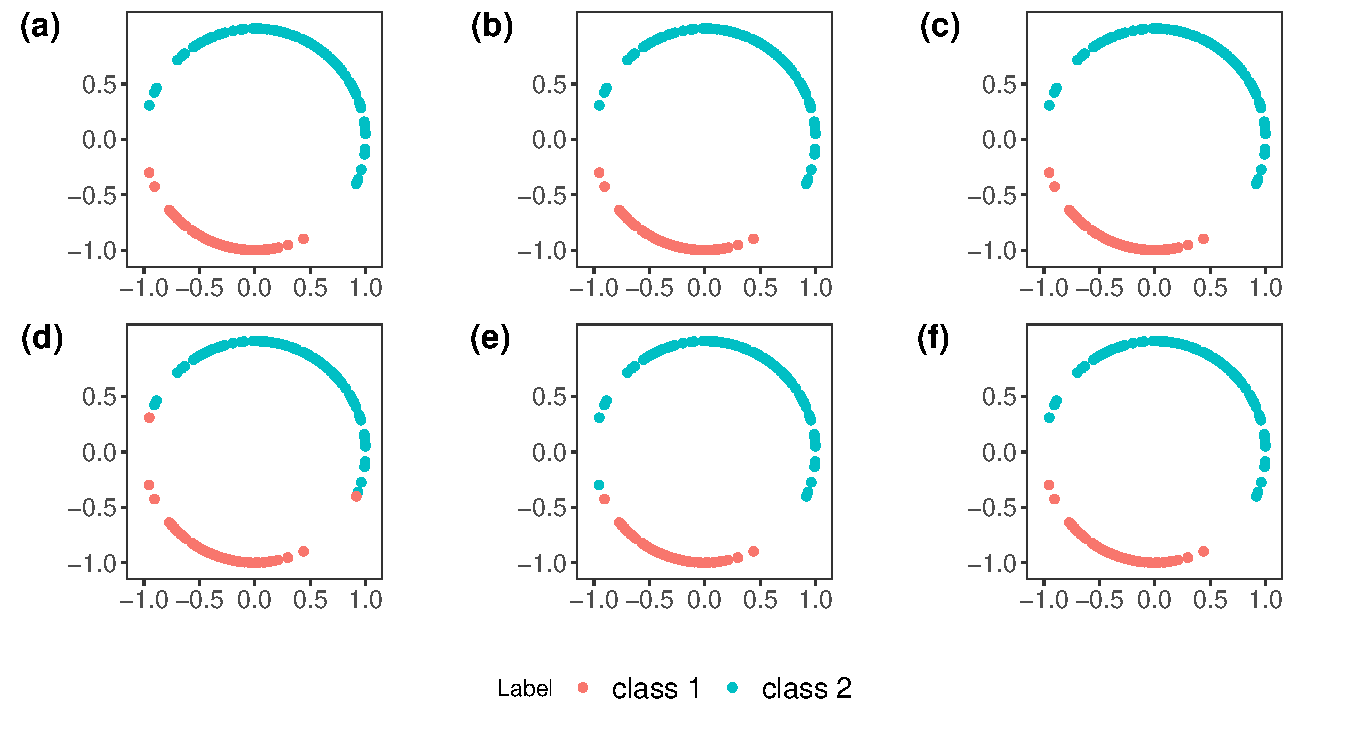
\includegraphics[width=0.95\linewidth]{figures/clust_smallmix-eps-converted-to.pdf}
	\vspace{-.2cm}
	\caption{Visualization of the \textsf{small-mix} example data consisting of two distinct classes on $\bbS^1$. The true label is shown in (a) and clustering results are given from the algorithms as follows; (b) \textsc{moSL}, (c) \textsc{kmeans}, (d) \textsc{spkmeans}, (e) \textsc{movMF}, and (f) \textsc{moSN} when the number of clusters is set as 2.}
	\label{fig:simulation_smallmix}
\end{figure}

We show a random sample with true label and clustering results in Fig. \ref{fig:simulation_smallmix}, where the true label is perfectly recovered from our proposed mixture of SL distributions along with $k$-means and SN mixture models. It is not surprising that the standard $k$-means algorithm achieves the perfect clustering since the sample has two distinct components. It was also reported in \cite{you_2022_ParameterEstimationModelbased} that the SN mixture outperforms spherical $k$-means and vMF mixture models, both of which misclassified observations near the boundary. We repeated the test 100 times and compared average clustering indices, which are summarized in Table \ref{table:small_mix}. When the true number of clusters is set as $K=2$, we witnessed an interesting phenomenon that the SL mixture is the best performing method even though the data was generated from the mixture of SN components. One  explanation of this phenomenon is related to robust estimation of cluster means for the SL distribution so that the perturbed observations at the boundary of two components less affect the overall identification of clusters. When the models are misspecified, the SL mixture returned smaller clustering comparison indices than other mixture models. Since the true partition is not known in most real cases, we consider this as an encouraging pattern since a valid mixture model should discourage misspecification.

\begin{table}[h]
	\caption{Average of clustering quality indices from 100 runs for the \textsf{small-mix} experiment. For each column, the cell containing bold-face numeric indicates that the corresponding row is the best performing model given the cluster number $K$ and quality index.}
	\label{table:small_mix}
	\vskip-0.3cm
	\smallskip
	\centering\small
	\begin{tabular}{cccccccccc}
		\hline
		\multirow{2}{*}{} & \multicolumn{3}{c}{Jaccard} & \multicolumn{3}{c}{Rand} & \multicolumn{3}{c}{NMI} \\ \cline{2-10} 
		& $K=2$     & $K=3$    & $K=4$    & $K=2$      & $K=3$     & $K=4$     & $K=2$   & $K=3$   & $K=4$    \\ \hline
		\textsc{moSL-soft} & \textbf{0.9862} & 0.7521 & 0.6107 & \textbf{0.9930} & 0.8756 & 0.8052 & \textbf{0.9712} & 0.7972 & 0.7194 \\ 
		\textsc{moSL-hard} & 0.9689 & 0.7430 & 0.5861 & 0.9841 & 0.8708 & 0.7926 & 0.9422 & 0.7848 & 0.7015 \\ 
		\textsc{kmeans} & 0.9575 & 0.7463 & 0.5588 & 0.9782 & 0.8726 & 0.7789 & 0.9270 & 0.7822 & 0.6930 \\ 
		\textsc{spkmeans} & 0.9465 & 0.7427 & 0.5997 & 0.9724 & 0.8709 & 0.7996 & 0.9118 & 0.7935 & 0.7104 \\ 
		\textsc{movMF} & 0.9852 & \textbf{0.7927} & \textbf{0.6841} & 0.9825 & \textbf{0.8963} & \textbf{0.8424} & 0.9607 & 0.8193 & \textbf{0.7582} \\ 
		\textsc{moSN} & 0.9853 & 0.7907 & 0.6325 & 0.9830 & 0.8953 & 0.8167 & 0.9627 & \textbf{0.8225} & 0.7335 \\  \hline
	\end{tabular}
\end{table}



We now turn to the real data example using \textsf{household} data, which is a survey data of household-level expenditures on several commodity groups among 40 individuals (20 males, 20 females) \cite{everitt_2010_HandbookStatisticalAnalyses}. Following the convention of \cite{hornik_2014_MovMFPackageFitting}, we extracted expenditures of three categories - food, housing, and service. Our interest is on the proportion of each category so that a profile vector is obtained by $\ell_1$ normalization and projected onto $\bbS^2$ by square-root transformation, which is a common practice in studying compositional data \cite{marron_2021_ObjectOrientedData}.



\begin{table}[]
	\caption{Clustering quality indices where the number of clusters varies for the \textsf{household} data projected onto $\bbS^2$ by square-root transformation of compositional data. For each column, the cells with bold-face numerics indicate that the corresponding row is 
		the best performing algorithm given the cluster number $K$ and quality index.}
	\label{table:household}
	%\caption{Mean clustering quality indices of 50 runs. For each column, the cell containing bold-face numeric indicates that the corresponding row is the best performing model given the cluster number $K$ and quality index. }
	\vskip-0.3cm
	\smallskip
	\centering\small
	\begin{tabular}{cccccccccc}
		\hline
		\multirow{2}{*}{} & \multicolumn{3}{c}{Jaccard} & \multicolumn{3}{c}{Rand} & \multicolumn{3}{c}{NMI} \\ \cline{2-10} 
		& $K=2$     & $K=3$    & $K=4$    & $K=2$      & $K=3$     & $K=4$     & $K=2$   & $K=3$   & $K=4$    \\ \hline
		\textsc{moSL-soft} & \textbf{1.0000} & 0.7275 & 0.6342 & \textbf{1.0000} & 0.8603 & \textbf{0.8218} & \textbf{1.0000} & 0.7244 & \textbf{0.7524} \\ 
		\textsc{moSL-hard} & 0.5920 & 0.7275 & 0.5363 & 0.7385 & 0.8603 & 0.7705 & 0.5105 & 0.7244 & 0.6546 \\ 
		\textsc{kmeans} & 0.5920 & \textbf{0.7789} & 0.5363 & 0.7385 & \textbf{0.8923} & 0.7705 & 0.5105 & \textbf{0.8331} & 0.6546 \\ 
		\textsc{spkmeans} & 0.5920 & \textbf{0.7789} & 0.5363 & 0.7385 & \textbf{0.8923} & 0.7705 & 0.5105 & \textbf{0.8331} & 0.6546 \\ 
		\textsc{movMF} & 0.9025 & 0.7275 & \textbf{0.6450} & 0.9500 & 0.8603 & 0.8179 & 0.8558 & 0.7244 & 0.6645 \\ 
		\textsc{moSN} & 0.5920 & 0.7275 & 0.5363 & 0.7385 & 0.8603 & 0.7705 & 0.5105 & 0.7244 & 0.6546 \\  \hline
	\end{tabular}
\end{table}

Similar to the \textsf{small-mix} example, we compared performance of 6 different algorithms for varying number of clusters with the projected \textsf{household} data. Quality of clustering performance was measured by regarding the gender label as ground-truth cluster label in that the true number of clusters is 2. Results are summarized in Table \ref{table:household}.  While the SL and vMF mixtures turned out to be the only models that recovered gender-separated clusters, it is worth to mention that our proposed SL mixture model with standard soft membership showed perfect clustering results when model was correctly specified. Comparative visualization of different clustering outputs is presented in Fig. \ref{fig:clust_household}. Contrary to the SL mixture that perfectly recovers the gender-separated classes, other methods show somewhat strange patterns. For example, both $k$-means and spherical $k$-means misclassified observations near the north pole as belonging to the same class with those near the equator. This may come from the fact that these algorithms do not acknowledge much for the  constrained geometry of the domain. This pattern is also witnessed in two mixture models of vMF and SN components that the distinct classes are seemingly contaminated by farthest points. This may be caused by the fact that data from the male group is much more dispersed than that of the female group. When the SL distribution was fitted separately, the females' expenditure data was distributed with $\hat{\sigma}_{\textrm{MLE}} = 0.0643$, which is much smaller than that of the male group with $\hat{\sigma}_{\textrm{MLE}} = 0.1426$. Since the scale parameter $\sigma$ amounts to variability within the data, this means that the male group, compared to the female group, is less concentrated and shows higher degree of heterogeneity. In reality, it is nearly impenetrable to distinguish presence of outliers from noise of substantial magnitude. Therefore, specifying a mixture model with robust components can help to deal with the scenario that we observed. 

\begin{figure}[h]
	\centering
	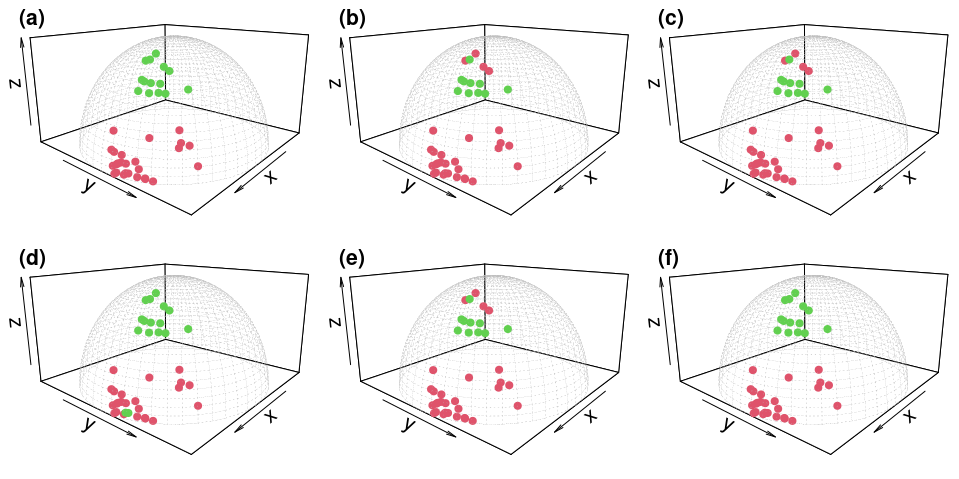
\includegraphics[width=0.95\linewidth]{figures/clust_household.png}
	\vspace{-.2cm}
	\caption{
		Visualization of the \textsf{household} data on $\bbS^2$. The true label defined by gender is shown in (a) and clustering results are given from the algorithms as follows; (b) \textsc{kmeans}, (c) \textsc{spkmeans}, (d) \textsc{movMF}, (e) \textsc{moSN}, and (f) \textsc{moSL}. All models for comparison are specified with the number of clusters as 2.}
	\label{fig:clust_household}
\end{figure}










%%%%%%%%%%%%%%%%%%%%%%%%%%%%%%%%%%%%%%%%%%%%%%%%%%%%%%%%%%%%%%%%%%%%%%%%%%%%%%%%%%%%%%%%%%%%%%%%%%%%%%
\section{Conclusions}\label{sec7:conclusion}

We proposed the SL distribution, a generalization of the Laplace distribution onto the unit hypersphere. The distribution was shown to be well-defined and provided with a sampling scheme, which is a fundamental tool arising in many computational pipelines. We showed that the maximum likelihood estimates of the governing parameters uniquely exist under mild conditions on the support of an empirical measure.  We also proposed  numerical optimization routines for maximum likelihood estimation of location and scale parameters since the SL distribution does not admit closed-form formulae for the estimates. The proposed algorithm is validated with extensive experiments using simulated data. An application of our proposal is model-based clustering of spherical data under the finite mixture framework where the components are SL distributions. Our experiments with simulated and real data showed that there is gain from the SL mixture  where a large amount of noise is suspected. 

We close by discussing several topics of interests for future studies. As noted before, the current sampling scheme built upon rejection sampler could be inefficient when a scale parameter is set to be very small. We expect that further investigation along this direction makes the proposed distribution a more appealing component not only for statistical inference but also for probabilistic deep learning such as variational autoencoders. Another line of research is reserved for refining clustering procedures. While our current exploration focuses on the finite mixture framework, availability of an effective sampler helps to open up opportunities such as a nonparametric Bayesian density estimation \cite{bhattacharya_2012_NonparametricBayesClassification} and modelling hierarchical and temporal data on the unit hypersphere  \cite{gopal_2014_MisesfisherClusteringModels}. The last direction is anisotropic extension of the SL distribution as done in \cite{hauberg_2018_DirectionalStatisticsSpherical} for the SN distribution, which will be beneficial in flexible modelling of directionally dependent data on the unit hypersphere. 




%%%%%%%%%%%%%%%%%%%%%%%%%%%%%%%%%%%%%%%%%%%%%%%%%%%%%%%%%%%%%%%%%%%%%%%%%%%%%%%%%%%%%%%%%%%%%%%%%%%%%%
\section*{Appendix}\label{sec:appendix}
We describe technical details on derivation of rejection sampler for the SL distribution. A standard rejection sampler aims at drawing random samples from a target density $f(\bfx)$ by samples from a proposal distribution $g(\bfx)$, assuming the likelihood ratio $f(\bfx)/g(\bfx)$ is upper bounded by some constant $M \in (1, \infty)$ over the entire domain. A draw from $g(\bfx)$ is accepted as a random sample from $f(\bfx)$ with probability $f(\bfx)/M g(\bfx)$ and the process is repeated until a successful draw. For the SL distribution with parameters $(\bfmu,\sigma) \in \bbS^p \times \bbRpos$, we consider the SN distribution of parameters $(\bfmu, 1/\sigma) \in \bbS^p \times \bbRpos$ as a proposal density. We note that density functions for SN and SL distributions are explicitly written as
\begin{equation*}
\fSN(\bfx~|~\bfmu,\lambda) = \frac{1}{Z_p(\lambda)} \exp \left(-\frac{\lambda}{2} d^2(\bfx,\bfmu)\right)\quad\text{and}\quad \fSL(\bfx~|~\bfmu,\sigma) = \frac{1}{C_p(\sigma)} \exp \left(-\frac{1}{\sigma} d(\bfx,\bfmu)\right),
\end{equation*}
for some normalizing constant $Z_p$ for the SN distribution \cite{hauberg_2018_DirectionalStatisticsSpherical}. Under the scenario, the likelihood ratio is given by
\begin{align*}
\frac{\fSL(\bfx~|~\bfmu,\sigma)}{\fSN(\bfx~|~\bfmu,\lambda)} &= 
\frac{Z_p (\lambda)}{C_p (\sigma)} \exp\left(-\frac{1}{\sigma}d(\bfx,\bfmu) + \frac{\lambda}{2} d^2(\bfx,\bfmu)\right)\\ 
&=
\frac{Z_p (1/\sigma)}{C_p (\sigma)} \exp\left(-\frac{1}{\sigma}d(\bfx,\bfmu) + \frac{1}{2\sigma} d^2(\bfx,\bfmu)\right)\\
&= \frac{Z_p (1/\sigma)}{C_p (\sigma)} \exp\left(\frac{(d(\bfx,\bfmu)-1)^2}{2\sigma}\right) \cdot  \exp\left(-\frac{1}{2\sigma}\right)\\  &\leq \frac{Z_p (1/\sigma)}{C_p (\sigma)} \exp\left(\frac{((\pi-1)^2}{2\sigma}\right) \cdot \exp\left(-\frac{1}{2\sigma}\right) =: M,
\end{align*}
where the constant $M$ is an upper bound of the ratio. An inequality comes from the fact that injectivity radius of a unit hypersphere is $\pi$, i.e., any two points on the unit hypersphere have distance of $\pi$ at most. Then, the corresponding probabilistic acceptance threshold $\tau$ is as follows;
\begin{align*}
\tau &= \frac{\fSL(\bfx~|~\bfmu,\sigma)}{M \fSN(\bfx~|~\bfmu,1/\sigma)}\\
&= \frac{C_p(\sigma)}{Z_p (1/\sigma)} 
\exp\left(-\frac{(\pi-1)^2}{2\sigma}\right) \cdot  \exp\left(\frac{1}{2\sigma}\right)\cdot 
\frac{1}{C_p(\sigma)} \exp\left(-\frac{d(\bfx,\bfmu)}{\sigma}\right) \cdot  Z_p (1/\sigma) \cdot  \exp\left(\frac{1}{2\sigma} d^2 (\bfx,\bfmu) \right)\\
&= \exp\left(\frac{1}{2\sigma}d^2 (\bfx,\bfmu) - \frac{1}{\sigma}d (\bfx,\bfmu) + \frac{1}{2\sigma}\right)\cdot \exp\left(-\frac{(\pi-1)^2}{2\sigma}\right)\\ &= \exp\left(\frac{(d(\bfx,\bfmu)-1)^2 - (\pi-1)^2}{2\sigma} \right).
\end{align*}


\bibliographystyle{dcu}
\bibliography{splaplace}
%%!TEX encoding = UTF-8 Unicode
\documentclass[11pt]{article}
\usepackage[usenames,dvipsnames,svgnames,table]{xcolor} % usenames : 16 basic colors,  dvipsnames : other 68 colors, svgnames : another 150 colors. It is used instead of \usepackage{color}. Can find descriptions for color in xcolor package. 

% algorithm
% (1) rename require/ensure https://en.wikibooks.org/wiki/LaTeX/Algorithms#Typesetting_using_the_algorithmic_package 
\usepackage{algorithm}
\usepackage{algorithmic}
\floatname{algorithm}{Algorithm}
\renewcommand{\algorithmicrequire}{\textbf{Input:}}
\renewcommand{\algorithmicensure}{\textbf{Output:}}

% table management
\usepackage{longtable}
\usepackage{hhline}
\usepackage{float}
\newfloat{algorithm}{tb}{lop}

\usepackage{enumitem} % for \begin{description}
\usepackage{rotfloat} % For [H] option in sidewaystable
\usepackage{graphicx}
\usepackage{epsfig}
\usepackage{amssymb, amsmath, amsthm}
\usepackage{verbatim}
\usepackage{natbib}
\usepackage{authblk}
%\usepackage{kotex}
\usepackage{multirow}
%\usepackage[colorlinks]{hyperref} 
\usepackage{subcaption} % for \begin{subtable}
\usepackage{array}
\newcolumntype{L}{>{\centering\arraybackslash}m{0.1\linewidth}}

\renewcommand{\baselinestretch}{1.25}

\newtheorem{theorem}{Theorem}[section]
\newtheorem{lemma}[theorem]{Lemma}
\newtheorem{proposition}[theorem]{Proposition}
\newtheorem{corollary}[theorem]{Corollary}
\newtheorem{fact}[theorem]{Fact}
\newtheorem{example}{Example}[section]
\newtheorem{definition}{Definition}






%\newenvironment{proof}[1][Proof]{\begin{trivlist}
%\item[\hskip \labelsep {\bfseries #1}]}{\end{trivlist}}
%\newenvironment{definition}[1][Definition]{\begin{trivlist}
%\item[\hskip \labelsep {\bfseries #1}]}{\end{trivlist}}
%\newenvironment{remark}[1][Remark]{\begin{trivlist}
%\item[\hskip \labelsep {\bfseries #1}]}{\end{trivlist}}



%\newcommand{\qed}{\nobreak \ifvmode \relax \else
%      \ifdim\lastskip<1.5em \hskip-\lastskip
%      \hskip1.5em plus0em minus0.5em \fi \nobreak
%      \vrule height0.75em width0.5em depth0.25em\fi}

%\def\qed{\space$\Box$ \par \vspace{.15in}}

% ***************************************************************
% Changed by Kisung You
\DeclareMathOperator*{\argmin}{argmin}
\DeclareMathOperator*{\argmax}{argmax}
\newcommand{\todokl}{\todo[inline,color=lime]}

\newcommand{\simiid}{\overset{iid}{\sim}}
\newcommand{\simind}{\overset{ind}{\sim}}

% arrows
\newcommand{\Lra}{\Longrightarrow}
\newcommand{\lra}{\longrightarrow}
\newcommand{\ra}{\rightarrow}

% caligraph
\newcommand{\calA}{\mathcal{A}}
\newcommand{\calB}{\mathcal{B}}
\newcommand{\calC}{\mathcal{C}}
\newcommand{\calD}{\mathcal{D}}
\newcommand{\calE}{\mathcal{E}}
\newcommand{\calF}{\mathcal{F}}
\newcommand{\calG}{\mathcal{G}}
\newcommand{\calH}{\mathcal{H}}
\newcommand{\calL}{\mathcal{L}}
\newcommand{\calM}{\mathcal{M}}
\newcommand{\calN}{\mathcal{N}}
\newcommand{\calP}{\mathcal{P}}
\newcommand{\calQ}{\mathcal{Q}}
\newcommand{\calS}{\mathcal{S}}
\newcommand{\calT}{\mathcal{T}}
\newcommand{\calU}{\mathcal{U}}
\newcommand{\calX}{\mathcal{X}}
\newcommand{\calY}{\mathcal{Y}} 
\newcommand{\calZ}{\mathcal{Z}}

% mathbb's
\newcommand{\bbG}{\mathbb{G}}
\newcommand{\bbP}{\mathbb{P}}
\newcommand{\bbQ}{\mathbb{Q}} 
\newcommand{\bbR}{\mathbb{R}}
\newcommand{\bbS}{\mathbb{S}}
\newcommand{\bbE}{\mathbb{E}}
\newcommand{\bbN}{\mathbb{N}}
\newcommand{\bbX}{\mathbb{X}}

% mathbf's
\newcommand{\bfS}{\mathbf{S}}
\newcommand{\bfX}{\mathbf{X}}
\newcommand{\bfZ}{\mathbf{Z}}
\newcommand{\bfLambda}{\mathbf{\Lambda}}
\newcommand{\bfTheta}{\mathbf{\Theta}}

% mathsf's
\newcommand{\sfD}{\mathsf{D}} % persistence diagram
\newcommand{\sfL}{\mathsf{L}} % persistence landscape
\newcommand{\sfC}{\mathsf{C}}   % Cech complex
\newcommand{\sfVR}{\mathsf{VR}} % Vietoris-Rips complex

% text notations
\newcommand{\ptcloudx}{\mathbb{X}} % Point cloud X
\newcommand{\ptcloudy}{\mathbb{Y}} % Point cloud Y

\newcommand{\Frechet}{Fr\'{e}chet }
\newcommand{\Hilbert}{L_2(\mathbb{N}\times \mathbb{R})}
\newcommand{\Erdos}{Erd\H{o}s}
\newcommand{\Renyi}{R\'{e}nyi }

\newcommand{\rmE}{\textrm{E}}
\newcommand{\rmVar}{\textrm{Var}}

% composite commands
\newcommand{\norm}[1]{\left\lVert#1\right\rVert}
\newcommand{\future}[1]{{\color{blue}\bf (#1)}}
\newcommand{\needref}[1]{{\bf (#1)}}

% collaborative works
\newcommand{\kisung}[1]{{\color{red}#1}}


% ***************************************************************

\parindent=15pt
\textheight 22cm \textwidth  16.5cm \oddsidemargin 0mm \topmargin     5mm
\headheight    0mm


\begin{document}
	
\title{Parameter Estimation and Model-Based Clustering with Spherical Normal Distribution on the Unit Hypersphere}
\author[1]{Kisung You}
\affil[1]{Department of ACMS, University of Notre Dame}
%\author[2]{Lizhen Lin}
%\affil[1,2]{Department of ACMS, University of Notre Dame}
\date{}

\maketitle
\begin{abstract}
In directional statistics, the von Mises-Fisher (vMF) distribution is one of the most basic and popular probability distributions for data on the unit hypersphere. Recently, the spherical normal (SN) distribution was proposed as an intrinsic counterpart to the vMF distribution by replacing the standard Euclidean norm with the great-circle distance, which is the shortest path joining two points on the unit sphere. We propose numerical approaches for parameter estimation since there are no analytic formula available. We consider the estimation problems in a general setting where non-negative weights are assigned to observations. This leads to a more interesting contribution for model-based clustering on the unit hypersphere by finite mixture model with SN distributions. We validate efficiency of optimization-based estimation procedures and effectiveness of SN mixture model using simulated and real data examples. 
\end{abstract}

%Key words: no keywords yet.


% ***************************************************************
\section{Introduction}\label{sec:intro}


Learning with data on Riemannian manifolds has attained much interests due to its capability that enables us exploit geometric structures of the underlying space behind the data \citep{bhattacharya_nonparametric_2012-1, patrangenaru_nonparametric_2016, pennec_riemannian_2020}. For example, the Stiefel and Grassmann manifolds, which are the spaces of orthonormal bases and subspaces, have been extensively used in computer vision community for applications such as face recognition \citep{aggarwal_system_2004}, shape analysis \citep{goodall_projective_1999}, and human pose modeling \citep{bissacco_recognition_2001}, to name a few. In medical image analysis, the manifold of symmetric and positive definite matrices has been employed for inferential tasks such as modeling anatomical variability in a population of brain scans \citep{fletcher_geometric_2009-1} and translating popular statistical tools for the space of functional brain connectivity \citep{you_re-visiting_2021}. 

In statistics, one of the long-standing disciplines to learn with manifold-valued data is directional statistics  \citep{mardia_directional_2000, ley_modern_2017-1}. As its name suggests, main objects in directional statistics include directions, axes, and rotations where the first two are represented by unit vectors and lines through the origin. Especially, the directions seem to attract the largest portion of attention in directional statistics for its ubiquity as many examples involve observations on the unit hypersphere.


The von Mises-Fisher (vMF) distribution is one of the most well-studied probability distributions on the unit hypersphere that belongs to a location-scale family \citep{fisher_dispersion_1953, mardia_directional_2000}. Given the $p$-dimensional random vector $x$, the probability density is given by
\begin{equation}\label{def:density_vMF}
f_{\text{vMF}}(x|\mu,\kappa) = C_p (\kappa) \exp (\kappa \mu^\top x)
\end{equation}
where $C_p (\kappa)$ is the normalizing constant and $(\mu,\kappa)$ are location and concentration parameters for the distribution. The vMF distribution is an exponential family in that it has played a foundational role in statistical inference for random variables on the unit hypersphere and has been extensively studied from a variety of aspects ranging from parameter estimation \citep{jupp_maximum_1979, sra_short_2012} to finite and nonparametric Bayesian clustering \citep{banerjee_clustering_2005,hornik_movmf_2014, bhattacharya_nonparametric_2012-2}.


It is straightforward to observe that the vMF distribution can be formulated in a similar fashion of the Gaussian distribution as follows,
\begin{equation*}
\exp \left( -\frac{\kappa}{2} \|x-\mu\|^2 \right) = \exp \left( -\frac{\kappa}{2} \left\lbrace x^\top x - 2\mu^\top x + \mu^\top \mu \right\rbrace \right) \propto \exp \left(\kappa \mu^\top x\right)
\end{equation*}
since both $x$ and $\mu$ are unit-norm vectors. In the context of manifold-valued data analysis, the use of Euclidean norm corresponds to the \emph{extrinsic} framework, where a distance between two objects is measured by a standard distance after equivariant embedding of the objects onto the Euclidean space \citep{bhattacharya_nonparametric_2012-1}. A counterpart in the dichotomy of geometric data analysis is the \emph{intrinsic} framework, which measures a distance via the shortest-path geodesic joining two points, which is the great circle on the unit hypersphere. Therefore, replacing the Euclidean norm with the great-circle distance gives a counterpart of the vMF distribution corresponds to the Riemannian normal law proposed in \cite{pennec_intrinsic_2006}. One motivation for such proposal comes from an observation that as two points are farther apart on the hypersphere, the extrinsic distance tends to understate the degree of distantness as shown in Figure \ref{fig:example_distance}.

\begin{figure}[ht]
	\centering
	
\includegraphics[width=0.99\linewidth]{figures/example_distance.eps}
	\caption{Distances for two points on the great circle displaced by angle $\theta$ under (a) intrinsic and (b) extrinsic frameworks.}
	\label{fig:example_distance}
\end{figure}

Recently, the spherical normal (SN) distribution was formally presented whose density is governed by the squared geodesic distance in the spirit of  intrinsic framework \citep{hauberg_directional_2018-1}. While anisotropic and isotropic versions of the SN distribution were originally proposed,  the former has less attractive aspects due to lack finite-time computation of the normalizing constant and complicated optimization routines for parameter estimation. On the other hand, an isotropic version has a closed-form expression of the normalizing constant and has a number of interesting connections to the well-established literature on manifold-valued data analysis. Throughout this work, we limit our focus on the isotropic SN distribution.

When given a proper probability distribution function, one of the first tasks for statistical inference is parameter estimation in the sense of maximum likelihood. Based on an observation that estimating the location parameter of the SN distribution is equivalent to the \Frechet mean estimation problem, we present an algorithm for a more general case where each observation is given a fixed weight independently. The concentration parameter estimation is a more challenging task because of the normalizing constant expressed in an integral form. Similar to the vMF distribution's case, we propose a numerical approach for estimation based on univariate optimization routines and approximation of derivatives via finite difference schemes. 


An important application of a probability distribution is model-based clustering \citep{bouveyron_model-based_2019}. The finite mixture model \citep{mclachlan_finite_2019} is one of the central tools in density estimation and model-based clustering by matching each observation to the cluster of maximal probability. Based on the aforementioned routines, we present the finite mixture of SN distributions where each component is the SN distribution, similar to the mixture of vMF distributions  \citep{banerjee_clustering_2005, hornik_movmf_2014}.




The rest of the paper is organized as follows. Section \ref{sec:preliminaries} reviews the elements of Riemannian geometry on the unit hypersphere and the SN distribution. Section \ref{sec:estimation} presents theoretical results regarding existence and uniqueness of the maximum likelihood estimates and numerical optimization routines for estimation. In Section \ref{sec:clustering}, We present computational routines of the SN mixture for clustering with some variants. We validate the algorithms with simulated and real data examples in Section \ref{sec:experiment}. We conclude in Section \ref{sec:conclusion} by discussing issues and directions for future studies. 



% ***************************************************************
\section{Preliminaries}\label{sec:preliminaries}


We start this section by introducing notations. Let $\bbS^p = \lbrace x \in \bbR^{p+1} : \|x\|_2 = 1 \rbrace $ denote a $p$-dimensional sphere in a $(p+1)$-dimensional Euclidean space $\bbR^{p+1}$. For a general metric space $(\bbX, d)$, we denote the open ball of radius $r > 0$ centered at a point $x \in \bbX$ as $B (x, \epsilon) := \lbrace y\in\bbX ~|~ d(x,y) < \epsilon \rbrace $. $\bbR^+$ stands for a set of strictly positive real numbers. For $x,y\in \bbS^p$, the distance $d(x,y)$ refers to the geodesic distance on the sphere while $\|x-y\|$ is the standard $L_2$ distance in an ambient Euclidean space $\bbR^{p+1}$. For the rest of this paper, several terms such as sphere, unit sphere, and unit hypersphere may be used interchangeably.


\subsection{Elements of Riemannian Geometry on the Sphere}

We first review some properties of the unit sphere as a Riemannian manifold along with explicit expressions of operations for computation \citep{absil_optimization_2008-1}. For an introduction and general exposition to Riemannian manifolds in detail, we refer interested readers to some standard references \citep{carmo_riemannian_1992, lee_riemannian_1997}.

The tangent space at $x \in \bbS^p$ is given by $T_x \bbS^p = \lbrace y \in \bbR^{p+1}:\langle x, y \rangle = 0\rbrace$ where $\langle \cdot, \cdot \rangle$ is a standard inner product. 
As a Riemannian manifold, $\calM = \bbS^p$ is equipped with a canonical metric $g_x (u,v) = \langle u, v \rangle$ for any $u,v \in T_x \bbS^p$. The unit sphere is known to have a positive constant sectional curvature of 1. The shortest path connecting two points $x,y \in \bbS^p$ is the great circle so that the distance between $x$ and $y$ is given by $d(x,y) = \cos^{-1}(\langle x, y \rangle)$. An exponential map is a map from a tangent space to a manifold itself and its inverse is called a logarithmic map, which are shown in Figure \ref{fig:maps}. For $x,y \in \bbS^p$ and $u \in T_x \bbS^p$, two maps are given as follows,
\begin{subequations}\label{eq:exp_log_maps}
\begin{align}
\text{Exp}_x (u) &= \cos (\|u\|) x + \frac{\sin(\|u\|)}{\|u\|} u \\
\text{Log}_x (y) &= \frac{d(x,y)}{\|\text{Proj}_x (y-x)\|} \text{Proj}_x (y-x)
\end{align}	
\end{subequations}
where $\text{Proj}_x (z) = z - \langle x, z \rangle x$ is a projection operator for a vector $z \in \bbR^{p+1}$ onto $T_x \bbS^p$. Finally, the injectivity radius, which is a maximal radius where the exponential map is a diffeomorphism, for the unit sphere is $\pi$. 

\begin{figure}[ht]
	\centering
	
\includegraphics[width=.5\linewidth]{figures/geometry.eps}
	\caption{Exponential and logarithmic maps on a Riemannian manifold $\calM$.}
	\label{fig:maps}
\end{figure}

\subsection{Spherical Normal Distribution}

As introduced before, we limit our focus on an isotropic version of the SN distribution that was formally presented in \cite{hauberg_directional_2018-1}. Given location and concentration parameters $\mu \in \bbS^p$ and $\lambda \in \bbR^+$, the density function of the SN distribution is given by 
\begin{equation}\label{def:density_SN}
f_{\textsf{SN}}(x|\mu,\lambda) = \frac{1}{Z_p(\lambda)} \exp \left(-\frac{\lambda}{2}d^2 (x,\mu)\right)
\end{equation}
where the normalizing constant $Z_p (\lambda)$ is given in an integral from by 
\begin{equation}\label{def:normalizing_constant}
\begin{split}
Z_p (\lambda) &= \int_{\bbS^p} \exp \left(-\frac{\lambda}{2}d^2 (x,\mu)\right) dx \\
&= A_{p-1} \int_{r=0}^{\pi} \exp\left(-\frac{\lambda r^2}{2}\right) \sin^{p-1}(r)dr
\end{split}
\end{equation}
where $A_{p-1} = 2\pi^{p/2}/\Gamma(p/2)$ is the hypervolume or surface area of $\bbS^{p-1}$ and $\Gamma(\cdot)$ is the standard Gamma function. Roughly speaking, the concentration parameter $\lambda$ is an inverse of variance in an epistemological sense as shown in Figure \ref{fig:example_density3} where a large $\lambda$ leads to concentrated mass at the vicinity of $\mu$ and a small $\lambda$ shows dispersed distribution of the mass over a larger support. 
\begin{figure}[ht]
	\centering
	\includegraphics[width=0.9\linewidth]{figures/example_density3.eps}
	\caption{Densities of the isotropic SN distributions on $\bbS^2$ with different concentration parameter values of (a) $\lambda=5$, (b) $\lambda=10$, and (c) $\lambda=20$}
	\label{fig:example_density3}
\end{figure}



\section{Maximum Likelihood Estimation}\label{sec:estimation}

Let $\bfX = \lbrace x_1, \ldots, x_n\rbrace$ a random sample on the unit sphere $\bbS^p$. The maximum likelihood estimates $(\hat{\mu}_{\text{MLE}}, \hat{\lambda}_{\text{MLE}}) \in \Theta = \bbS^p \times \bbR^+$ are obtained by maximizing the following log-likelihood function
\begin{equation}\label{def:lkd}
\begin{split}
L(\mu,\lambda; \bfX) &= \sum_{i=1}^n \log \left\lbrace \frac{1}{Z_p(\lambda)} \exp \left(-\frac{\lambda}{2}d^2(x_i,\mu)\right)\right\rbrace\\ 
&= -\frac{\lambda}{2}\sum_{i=1}^n d^2 (x_n,\mu) - n\log Z_p(\lambda)
\end{split}
\end{equation}
which does not admit closed-form solutions due to the existence of nonlinear terms in a likelihood function hence necessitates to employ numerical optimization. To briefly describe the strategy for both theory and computation, we recognize that the constrained maximization of Equation \eqref{def:lkd} with respect to $\mu$ does not depend on the concentration parameter,
\begin{equation}\label{def:problem_mu}
\hat{\mu}_{\text{MLE}} = \underset{\mu \in \bbS^p}{\argmax} -\frac{\lambda}{2} \sum_{i=1}^n d^2(x_i,\mu) = \underset{\mu \in \bbS^p}{\argmin} \sum_{i=1}^n  d^2 (x_i, \mu)
\end{equation}
where the above equation has long been known as  \Frechet or Karcher mean problem \citep{frechet_les_1948, grove_how_1973-1, afsari_riemannian_2011}.  Given $\hat{\mu}$, solving for $\hat{\lambda}$ reduces to the following optimization problem
\begin{equation}\label{def:problem_lambda}
\hat{\lambda}_{\text{MLE}} = \underset{\lambda \in \bbR^+}{\argmax} -\frac{\lambda}{2} \sum_{i=1}^n d^2(x_i,\hat{\mu}) - n \log Z_p(\lambda) =  \underset{\lambda \in \bbR^+}{\argmin} ~\hat{C} \lambda + \log Z_p (\lambda)
\end{equation}
for a known positive constant $\hat{C} = \sum_{i=1}^n d^2(x_i,\hat{\mu}_{\text{MLE}})/2n$. The following theorem shows existence and uniqueness of maximum likelihood estimates.

\begin{theorem}\label{thm:hadamard}
	Let $x_1,x_2,\ldots,x_n$ be a random sample on $\bbS^p$ that are contained in an open geodesic ball $B(x, \pi/2)$ for some $x \in \bbS^p$. Then, maximum likelihood estimates of $(\mu,\lambda)$ uniquely exist. 
\end{theorem} 
\begin{proof}
	The existence and uniqueness of $\hat{\mu}$ has been well-studied on a general Riemannian manifold $\calM$ \citep{kendall_probability_1990-1, nielsen_medians_2013}. Let $r^* = \min \lbrace \text{inj}(\calM), \pi/\sqrt{\bar{C}} \rbrace$ where $\bar{C}$ is the least upper bound of sectional curvatures of $\calM$.  Proposition 5.2 of \cite{bhattacharya_nonparametric_2012-1} states that if a measure $Q= (1/n) \sum_{i=1}^n \delta_{x_i}$ on $\calM$ has support in $B(x, r^*/2)$ for some $x \in \bbS^p$, then $Q$ has a unique local sample mean inside the ball. On the sphere $\calM = \bbS^p$, twice the convexity radius is $r^* = \min \lbrace \pi, \pi/1 \rbrace = \pi$, which proves the existence and uniqueness of $\hat{\mu}_{\text{MLE}}$.
	
	For $\hat{\lambda}_{\text{MLE}}$, we first show that there exists a unique critical point of the Equation \eqref{def:problem_lambda}, which specifies the likelihood in an equivalent form. Let $g(\lambda) = \hat{C} \lambda + \log Z_p (\lambda)$ with a known constant $\hat{C} = \sum_{i=1}^n d^2 (x_i, \hat{\mu}_{\text{MLE}}) / 2n$ where $\hat{C} \in \lbrack 0, \frac{\pi^2}{2}\rbrack$ since the geodesic distance between any two points on the unit sphere is upper bounded by the injectivity radius $\pi$. Since $g'(\lambda) = 0$ if and only if $\hat{C} Z_p (\lambda) + Z_p ' (\lambda) = 0$, it suffices to show that $T(C) = C Z_p (\lambda) + Z_p '(\lambda)$ has a unique solution in $( 0, \frac{\pi^2}{2} )$ for any given $\lambda$. This implies a bijection between $\lambda$ and $C$ upon which the existence and uniqueness of a critical point for $g(\lambda)$ is established. First, we have $T(0) < 0$ since 
	\begin{equation}\label{eq:auxiliary}
	T(C) = A_{p-1} \int_{r=0}^\pi \left(C - \frac{r^2}{2}\right) \exp\left(-\frac{\lambda r^2}{2}\right) \sin^{p-1}(r)dr
	\end{equation}
	and $T(\frac{\pi^2}{2}) > 0$ as $C - \frac{r^2}{2} = \frac{\pi^2 - r^2}{2} >= 0$ on the domain. Second, it is trivial that $T(C)$ is continuous as the integrand consists of smooth and bounded functions on a finite interval. Furthermore, $T(C)$ is a monotonically increasing function since for any $C' > C$,
	\begin{equation*}
	T(C')-T(C) = A_{p-1} \int_{r=0}^\pi \left(C'-C\right) \exp\left(-\frac{\lambda r^2}{2}\right) \sin^{p-1}(r)dr > 0.
	\end{equation*}
	Therefore, by the intermediate value theorem and  monotonicity, $T(C)$ has a unique zero in $( 0, \frac{\pi^2}{2} )$ and so does $g'(\lambda)$.
	
	Let $\lambda^*$ be a unique critical point of $g(\lambda)$ and the rest is to show whether $\lambda^*$ is a local minimum. This is attained by comparing $g(\lambda^*+\epsilon)$ and $g(\lambda^* - \epsilon)$ with $g(\lambda^*)$ for $ \forall \epsilon > 0$. First, 
	\begin{align*}
	g(\lambda^* + \epsilon) &= \hat{C} (\lambda^* + \epsilon) + \log Z_p (\lambda^* + \epsilon) > \hat{C} \lambda^* + \hat{C} \epsilon + \log Z_p(\lambda^*) - \frac{\pi^2 \epsilon}{2} = g(\lambda^*) + \epsilon \left(\hat{C} - \frac{\pi^2}{2}\right)
	\end{align*}
	where $\hat{C} - \pi^2/2 \leq 0$. Similary, we have
	\begin{equation*}
	g(\lambda^*-\epsilon) = \hat{C}(\lambda^*-\epsilon) + \log Z_p (\lambda^* - \epsilon) > \hat{C}\lambda^* + \log Z_p (\lambda^*) - C\epsilon = g(\lambda^*) - \hat{C}\epsilon.
	\end{equation*}
	Since both inequalities hold for arbitrarily small $\epsilon$, taking the limit inferior as $\epsilon \rightarrow 0$ gives that both $g(\lambda^*+\epsilon)$ and $g(\lambda^*-\epsilon)$ are greater than $g(\lambda^*)$. Therefore, $g(\lambda)$ attains the minimum at $\lambda = \lambda^*$. 
\end{proof}


We note that the support condition $B(x,\pi/2)$ is natural especially when the manifold of interest is the unit sphere. If we consider north and south poles $\bbS^2$, there exist an infinite number of points along the equator that minimize the sum of squared distances.




\subsection{Estimating the Location}

It was observed from Equation \eqref{def:problem_mu} that  maximum likelihood estimation of $\mu$ is equivalent to the \Frechet mean problem that minimizes sum of squared distances. We illustrate a more general case of weighted \Frechet mean problem for future use in fitting a mixture model. Given a random sample $ \bfX = \lbrace x_1, \ldots, x_n \rbrace$ and non-negative weights $\mathbf{w} = \lbrace w_1, \ldots, w_n\rbrace$, the weighted \Frechet mean problem is given by
\begin{equation}\label{def:problem_weighted_frechet}
\underset{\mu\in\bbS^p}{\min}~f(\mu| \bfX, \mathbf{w}) = \underset{\mu\in\bbS^p}{\min}~ \sum_{i=1}^n w_i d^2 (x_i, \mu)
\end{equation}
hence the maximum likelihood estimate $\hat{\mu}_{\text{MLE}}$ is a solution to the special case of Equation \eqref{def:problem_weighted_frechet} when all weights $w_i$'s are set equal such as $w_i = 1/n$ from an empirical measure point of view. 

The hands-on choice in optimization on manifolds is Riemannian gradient descent \citep{absil_optimization_2008-1}. The gradient descent algorithm for a function $f (x) :\bbR^d \rightarrow \bbR$ evolves iterates along a path characterized by local gradient evaluations, i.e., $x^{(t+1)} = x^{(t)} - \alpha \nabla f (x^{(t)}) $ for some step-size $\alpha$. For a scalar-valued function on a Riemannian manifold $\calM$, the gradient is formerly defined as a vector field. This means for each point $p \in \calM$, $\text{grad} f \rvert_p$ is a tangent vector in $T_p \calM$ so that the resulting update rule requires an additional step to push at iterate tangent vector onto $\calM$ using an exponential map. Since $\text{grad} ~d^2 (x,y) = -2 \textrm{Log}_x y$ for $x,y \in \calM$ which can be easily shown using the variation of energy, we can write the gradient of Equation \eqref{def:problem_weighted_frechet} at iteration $t$ as 
\begin{equation*}
\text{grad} f \rvert_{\mu^{(t)}} = -2 \sum_{i=1}^n w_i \text{Log}_{\mu^{(t)}} (x_i)
\end{equation*}
and the final updating rule is given by 
\begin{equation*}
\mu^{(t+1)} \leftarrow \text{Exp}_{\mu^{(t)}} \left( 2\alpha^{(t)}  \sum_{i=1}^n w_i \text{Log}_{\mu^{(t)}} (x_i) \right)
\end{equation*}
for an initial point $\mu^{(0)}$ and step-size $\alpha^{(t)}$. Explicit forms for exponential and logarithmic maps are given in Equations \eqref{eq:exp_log_maps} and the procedure for location estimation is summarized in Algorithm \ref{code:lkd_mean}. 

\begin{algorithm}
	\caption{Weighted \Frechet mean computation}
	\label{code:lkd_mean}
	\begin{algorithmic}
		\REQUIRE a random sample $\lbrace x_1,\ldots,x_n\rbrace \subset \bbS^p$, weights $\lbrace w_1, \ldots, w_n\rbrace$, stopping criterion $\epsilon$.
		\ENSURE $\hat{\mu} = \argmin f(\mu)$ where $f(\mu) =  \sum_{i=1}^n w_i d^2 (x_i, \mu)$ for $\mu \in \bbS^p$. 
		\STATE Initialize $\mu^{(0)} = \sum_{i=1}^n w_i x_i / \| \sum_{i=1}^n w_i x_i\|$.
		\REPEAT 
			\STATE $\nabla f \vert_{\mu^{(t)}} \leftarrow -2 \sum_{i=1}^n w_i \text{Log}_{\mu^{(t)}} (x_i)$ 
			\STATE $\mu^{(t+1)} \leftarrow \text{Exp}_{\mu^{(t)}} \left( -\alpha^{(t)} \nabla f \vert_{\mu^{(t)}} \right)$
		\UNTIL $\|\nabla f \vert_{\mu^{(t)}} \| < \epsilon$ or $\| \mu^{(t)} - \mu^{(t+1)} \| < \epsilon$ .
	\end{algorithmic}
\end{algorithm}


We illustrate components of the Algorithm \ref{code:lkd_mean}. First, we use an initial starting point $\mu^{(0)} = \sum_{i=1}^n w_i x_i / \| \sum_{i=1}^n w_i x_i\|$. When $w_i$'s are all equal, this corresponds to an extrinsic mean \citep{bhattacharya_nonparametric_2012-1} or an estimate for a location parameter of the vMF distribution. When the support condition of Theorem \ref{thm:hadamard} is satisfied, estimates of both extrinsic and intrinsic means are contained in a convex geodesic ball. In addition to computational benefit that obtaining an extrinsic mean involves addition of vectors and $L_2$ normalization, it is a reasonable choice of starting point to have a small number of iterations for convergence. Second, the step-size parameter $\alpha^{(t)}$ can be determined by line search or simply set as a fixed scalar. The latter strategy was used in Algorithm 1 of \cite{hauberg_directional_2018-1} with $\alpha=0.25$. This approach has trade-offs in the sense that a fixed step-size may incur additional iterations while it avoids repetitive evaluations of the objective function during a single line search. Finally, the stopping criterion $\|\nabla f \vert_{\mu^{(t)}} \| < \epsilon$ is motivated from the fact that $d^2(x,y) = \| \text{Log}_x y \|^2$ for $x,y\in \bbS^p$ with the canonical metric. Also $\| \mu^{(t)} - \mu^{(t+1)}\|$ is justified from the fact that for a Riemannian manifold $\calM$ embedded in Euclidean space, intrinsic and extrinsic distances converge as two points get sufficiently close, i.e.,  $\lim_{x\rightarrow y} d (x,y)/\|x-y\| =1$.







\subsection{Estimating the Concentration}

The maximum likelihood estimation for concentration parameter $\lambda$ is equivalent to solve the following optimization problem
\begin{equation*}
\hat{\lambda}_{\text{MLE}} =\underset{\lambda \in \bbR^+}{\argmin} ~ g(\lambda) \text{ where } g(\lambda) =\hat{C} \lambda + \log Z_p (\lambda)\text{ and } \hat{C} = \frac{1}{2n} \sum_{i=1}^n d^2(x_i, \hat{\mu}_{\text{MLE}})
\end{equation*}
Theorem \ref{thm:hadamard} showed that the problem \eqref{def:problem_lambda} has a unique critical point so that the optimization with respect to $\lambda$ can be cast as a  root-finding problem of $g'(\lambda)=0$. 

Householder's method is a class of univariate root-finding algorithms when the target function is $d$ times continuously differentiable \citep{householder_numerical_1970}. For solving $f(x)=0$ where the function has continuous derivatives up to order $d$, the method iterates by
\begin{equation}\label{algorithm:householder}
x^{(t+1)} \leftarrow  x^{(t)} + d \frac{(1/f)^{(d-1)} (x^{(t)})}{(1/f)^{(d)} (x^{(t)})}
\end{equation}
starting from an initial point $x^{(0)}$. For low orders $d=1$ and $2$, the updating rule in Equation \eqref{algorithm:householder} translates to those found from the Newton's and Halley's method, respectively. Therefore, we derive the updating rules to solve $g'(\lambda)=0$ using Householder's methods of orders 1 and 2 as follows,
\begin{subequations}\label{algorithm:householder_ordered}
\begin{align}
(\textrm{exact Newton's}) \quad&
\lambda^{(t+1)} \leftarrow  \lambda^{(t)} - \frac{g' (\lambda^{(t)})}{g'' (\lambda^{(t)})}  \label{algorithm:householder_newton}\\
(\textrm{exact Halley's}) \quad & \lambda^{(t+1)} \leftarrow \lambda^{(t)} - \frac{2g'(\lambda^{(t)}) g''(\lambda^{(t)})}{2 g'' (\lambda^{(t)})^2 - g'(\lambda^{(t)}) g'''(\lambda^{(t)})}  \label{algorithm:householder_halley}
\end{align}
\end{subequations}
beginning with an initial guess $\lambda^{(0)} \in \bbR^+$. 

Both updating rules involve evaluation of derivatives up to order 2 or 3 at each iteration, which may incur numerical instabilities due to computational reasons such as integrating high-order terms and others. %For example, if we simply write $Z $ for $Z_p (\lambda)$, we have $g'''(\lambda) = \lbrace Z^2 (Z' Z'' + Z Z''') - 2 (Z')^2\rbrace/Z^3$. 
In order to make computation more robust, we  employ the centered finite difference schemes using the five-point utensil 
\begin{subequations}\label{algorithm:utensil}
	\begin{align}
	g'(\lambda) &= \frac{g(\lambda+h) - g(\lambda-h)}{2h} =: \frac{A}{2h} \\
	g''(\lambda) &= \frac{g(\lambda+h)-2g(\lambda)+g(\lambda-h)}{h^2} =: \frac{B}{h^2} \\
	g'''(\lambda) &= \frac{g(\lambda+2h)-2g(\lambda+h)+2g(\lambda-h)-g(\lambda-2h)}{2h^3} =: \frac{C}{2h^3}
	\end{align}
\end{subequations}
for a sufficiently small step-size $h>0$ and the derivatives are approximated by a term of order $h^2$ \citep{burden_numerical_2016}. By plugging in the approximate derivatives \eqref{algorithm:utensil} to the updating rules in Equations \eqref{algorithm:householder_ordered}, we get
\begin{align}
(\textrm{approximate Newton's}) \quad&
\lambda^{(t+1)} \leftarrow  \lambda^{(t)} - \frac{h}{2} \left(\frac{A^{(t)}}{B^{(t)}}\right) \label{algorithm:final_newton}\\
(\textrm{approximate Halley's}) \quad & \lambda^{(t+1)} \leftarrow \lambda^{(t)} - 4h \left(\frac{
	A^{(t)}B^{(t)}
}{
8 (B^{(t)})^2 - A^{(t)}C^{(t)}
}\right)  \label{algorithm:final_halley}
\end{align}
where $A^{(t)} = g(\lambda^{(t)}+h) - g(\lambda^{(t)}-h)$ and others defined similarly. 

\begin{algorithm}
	\caption{Maximum likelihood estimation of the concentration parameter}
	\label{code:lkd_lambda}
	\begin{algorithmic}
		\REQUIRE a random sample $\lbrace x_1,\ldots,x_n\rbrace \subset \bbS^p$, a constant $C$, step-size $h$, stopping criterion $\epsilon$.
		\ENSURE $\hat{\lambda} = \argmin g(\lambda)$ where $g(\lambda) = C \lambda + \log Z_p (\lambda)$		
		\STATE Initialize $\lambda^{(0)}$.
		\REPEAT 
		\STATE Update $\lambda^{(t+1)}$ by either Newton's  \eqref{algorithm:final_newton} or Halley's \eqref{algorithm:final_halley} method.
		\UNTIL $|\lambda^{(t)} - \lambda^{(t+1)}|<\epsilon$.
	\end{algorithmic}
\end{algorithm}



We close this section by noting that computational complexities of the exact and approximate methods are compatible. At each iteration, the approximate Newton's method shown in Equation \eqref{algorithm:final_newton} requires 3 integral evaluations, which is same as that of the exact Newton's method \eqref{algorithm:householder_newton}. While the exact Halley's method \eqref{algorithm:householder_halley} evaluates $Z_p^{(k)} (\lambda)$ for $k = 0,\ldots,3$, the approximate Halley's algorithm requires an additional integral computation to evaluates five points around $\lambda^{(t)}$. However, the added computational cost is very thin since the integrand well behaves and the domain of integration is small. 




\section{Model-Based Clustering}\label{sec:clustering}

One of the most popular probabilistic clustering methods is finite mixture models \citep{mclachlan_finite_2019}. The density of a finite mixture model with $K$ SN components is given by
\begin{equation*}
h(x|\bfTheta) = \sum_{k=1}^K \pi_k f_{\textsf{SN}}(x|\mu_k,\lambda_k)
\end{equation*}
where $\pi_k \in [0,1]$ and $\sum_{k=1}^K \pi_k = 1$ with parameters $\bfTheta = \lbrace \pi_k, \mu_k, \lambda_k\rbrace_{k=1}^K$. For a random sample $\bfX = \lbrace x_1,x_2,\ldots,x_N\rbrace$ on the unit sphere, the log-likelihood is written as 
\begin{equation}\label{clustering:loglkd_naive}
\log P(\bfX|\bfTheta) = \sum_{n=1}^N \log h(x_n|\bfTheta) = \sum_{n=1}^N \log \left( \sum_{k=1}^K \pi_k f_{\textsf{SN}}(x_n|\mu_k,\lambda_k) \right).
\end{equation} The standard approach to maximize Equation \eqref{clustering:loglkd_naive} is to use Expectation-Maximization (EM) algorithm \citep{dempster_maximum_1977} by introducing latent variables for class membership. We leave detailed description of the technique to standard references in machine learning \citep{bishop_pattern_2006, hastie_elements_2009-1}. Let $\bfZ \in \lbrace 0, 1 \rbrace^{N\times K}$ be a 0-1 matrix of class memberships such that  $\sum_{k=1}^K z_{nk} = 1$ for all $n=1,\ldots,N$. Then, a joint distribution of $\bfX$ and $\bfZ$ is 
\begin{equation}\label{clustering:joint_density}
P(\bfX, \bfZ | \bfTheta) = \prod_{n=1}^{N} \prod_{k=1}^{K} \left\lbrace \pi_k f_{\textsf{SN}}(x_n\vert \mu_k, \lambda_k) \right\rbrace^{z_{nk}}
\end{equation}
Given an initial setting for the parameters $\bfTheta^{(0)}$, EM algorithm alternates the following two steps. In the E-step, the posterior distribution $P(\bfZ\vert \bfX, \bfTheta^{(t)})$ is evaluated to compute the complete-data log likelihood $Q(\bfTheta; \bfTheta^{(t)}) = \bbE_{\bfZ \vert \bfX, \bfTheta^{(t)}} \lbrack \log P(\bfX, \bfZ \vert \bfTheta)\rbrack = \sum_{\bfZ} P (\bfZ \vert \bfX, \bfTheta^{(t)}) \log P(\bfX, \bfZ \vert \bfTheta)$. The M-step attains a new iterate $\bfTheta^{(t+1)}$ by maximizing $Q(\bfTheta; \bfTheta^{(t)})$. 


We first present a standard EM algorithm and elaborate on explicit expressions for updating rules. At iteration $t$, the E-step reduces to evaluating $\bbE[z_{nk}]$ that has a universal form for mixture models,
\begin{equation}\label{clustering:Estep_soft}
\gamma_{nk} := \bbE[z_{nk}] = \frac{\pi_k^{(t)} f_{\textsf{SN}} (x_n\vert \mu_k^{(t)}, \lambda_k^{(t)})}{\sum_{j=1}^K \pi_j^{(t)} f_{\textsf{SN}} (x_n\vert \mu_j^{(t)}, \lambda_j^{(t)})}
\end{equation}
for $n=1,\ldots,N$ and $k=1,\ldots,K$. The matrix $\Gamma := \gamma_{nk} \in [0,1]^{N\times K}$ is called a soft clustering or membership matrix which encodes the probability of an observation $x_n$ belonging to the $k$-th cluster. This leads to the complete-data log likelihood at iteration $t$,
\begin{equation}\label{clustering:rule_M_equation}
Q(\bfTheta; \bfTheta^{(t)}) = \sum_{n=1}^N \sum_{k=1}^K \gamma_{nk} \left\lbrace \log \pi_k + \log f_{\textsf{SN}} (x_n\vert \mu_k, \lambda_k) \right\rbrace.
\end{equation}

The M-step maximizes Equation \eqref{clustering:rule_M_equation} by the following update rules. The weight parameters $\pi_k$'s are updated by
\begin{equation}\label{clustering:rule_M_weight}
\pi_k^{{(t+1)}} = \frac{\sum_{n=1}^N \gamma_{nk}}{N}\quad\text{  for }~k=1,\ldots,K
\end{equation}
using the method of Lagrange multipliers to handle the equality constraint $\sum_{k=1}^K \pi_k = 1$. 
Other parameters do not admit closed-form expressions in that they are obtained by numerical optimization introduced in Section \ref{sec:estimation}. The location parameters $\mu_k$'s are solutions of weighted \Frechet mean problem 
\begin{equation}\label{clustering:rule_M_location}
\mu_k^{(t+1)} = \underset{\mu \in \bbS^p}{\argmin} \sum_{n=1}^N  \gamma_{nk} \cdot d^2(x_n, \mu) 
\end{equation}
which can be solved by Algorithm \ref{code:lkd_mean} with weights $w_i = \gamma_{ik},~i=1,\ldots,n$. Similarly, the concentration parameters are solutions of the following problems,
\begin{subequations}\label{clustering:rule_M_concentration}
	\begin{equation}
	\lambda_k^{(t+1)} = \underset{\lambda \in \bbR^+}{\argmin}~
	\left( \frac{\sum_{n=1}^N d^2(\mu_k^{(t+1)}, x_n) \cdot \gamma_{nk}}{ 2 \sum_{n=1}^N \gamma_{nk}} \right) \lambda + \log Z_p (\lambda) \label{clustering:rule_M_concentration_hetero}
	\end{equation}
	for $k=1,\ldots,K$. When all concentration parameters $\lambda_1,\ldots,\lambda_K$ are required to be equal, the model is called homogeneous and the update rule for a common $\lambda$ is as follows,
	\begin{equation}
	\lambda^{(t+1)} =\underset{\lambda \in \bbR^+}{\argmin}~ \left( \frac{1}{2N}\sum_{n=1}^N \sum_{k=1}^K d^2 (\mu_k^{(t+1)}, x_n)\cdot\gamma_{nk} \right)\lambda +  \log Z_p(\lambda). \label{clustering:rule_M_concentration_homo}
	\end{equation}
\end{subequations}
where for both cases the update can be computed by Algorithm \ref{code:lkd_lambda} with the constant term changing along the iterations. 


From Equations \eqref{clustering:rule_M_location} and \eqref{clustering:rule_M_concentration}, we can observe that the large number of observations $N$ intensifies computational costs for parameter estimation. We present hard and stochastic assignment heuristics that manipulate a clustering membership matrix $\Gamma$ that represents distribution of the hidden variables. Let the $n$-th row of $\Gamma$ be denoted as $\Gamma_n = [\gamma_{n1},\ldots,\gamma_{nK}]$. The hard assignment is given by
\begin{equation}\label{clustering:Estep_hard}
\textsf{hard}(\gamma_{nk}) = \left. 
\begin{cases}
1, & \text{if $k$ is an index for maximum of $\Gamma_n$,}\\
0, & \text{otherwise}
\end{cases}
\right.
\end{equation}
and the stochastic assignment is similarly written as 
\begin{equation}\label{clustering:Estep_stochastic}
\textsf{stochastic}(\gamma_{nk}) = \left.
\begin{cases}
1, & \text{if $k$ = \textsf{sample}($1:K$, probability=$\Gamma_n)$}\\
0, & \text{otherwise}
\end{cases}
\right.
\end{equation}
where the \textsf{sample} procedure draws a random integer-valued index from 1 to K with probability $\Gamma_n$. Both heuristics aim at making $\Gamma$ sparse. Given a large number of observations, this helps significantly reduce intermediate evaluations and space complexity in update rules for both concentration and location parameters. Furthermore, hard assignment has proven to be optimal in the sense that the scheme maximizes a lower bound on the incomplete-data log likelihood \citep{banerjee_clustering_2005}. The complete procedure is summarized in Algorithm \ref{code:em_spnorm}. 




\begin{algorithm}[!t]
	\caption{EM algorithm for mixture of spherical normal distributions.}
	\label{code:em_spnorm}
	\begin{algorithmic}
		\REQUIRE a random sample $\lbrace x_1,\ldots,x_N\rbrace \subset \bbS^p$, number of clusters $K$.
		\ENSURE a clustering membership matrix $\Gamma$.		
		\STATE Initialize $ \bfTheta^{(0)} = \lbrace \pi_k, \mu_k, \lambda_k\rbrace_{k=1}^K$.
		\REPEAT 
			\STATE \{E-step\}
			\FOR{$n=1:N$}
				\FOR {$k=1:K$ }
				\STATE $\Gamma (n,k)= \pi_k^{(t)} f_{\textsf{SN}} (x_n\vert \mu_k^{(t)}, \lambda_k^{(t)})$
				\ENDFOR
				\STATE $\Gamma(n,:) = \Gamma(n,:)/ \sum_{k=1}^K \Gamma(n,k)$
			\ENDFOR 
			\STATE \{Heuristics\}
			\IF {hard assignment}
				\STATE $\Gamma \leftarrow \textsf{hard}(\Gamma)$ by Equation \eqref{clustering:Estep_hard}.
			\ELSIF {stochastic assignment}
				\STATE $\Gamma \leftarrow \textsf{stochastic}(\Gamma)$ by Equation \eqref{clustering:Estep_stochastic}.
			\ENDIF
			\STATE \{M-step\}
			\FOR{$k=1:K$}
				\STATE $\pi_k^{(t+1)} = \sum_{n=1}^N \gamma_{nk} / N$.
				\STATE $\mu_k^{(t+1)} = \underset{\mu \in \bbS^p}{\argmin}  \sum_{n=1}^N \gamma_{nk} \cdot d^2 (x_n, \mu)$ by Algorithm \ref{code:lkd_mean}.
			\ENDFOR
			\IF {homogeneous concentration}
				\STATE compute $\lambda^{(t+1)}$ by Equation \eqref{clustering:rule_M_concentration_homo}.
			\ELSE
				\FOR {$k=1:K$}
					\STATE  compute $\lambda_k^{(t+1)}$ by Equation
					\eqref{clustering:rule_M_concentration_hetero}.
				\ENDFOR
			\ENDIF
		\UNTIL convergence.
	\end{algorithmic}
\end{algorithm}

We describe a few practical details of the EM algorithm. The algorithm is first initialized with standard $k$-means clustering \citep{macqueen_methods_1967, hornik_movmf_2014} since there exist a number of fast and efficient implementations of the standard $k$-means algorithm. Furthermore, an equivariant embedding on the sphere that preserves a large amount of geometric information is the identity map \citep{bhattacharya_nonparametric_2012-1}, which may justify the scheme by arguing that some degree of geometric information is preserved. Second, one popular choice for the termination criterion is to run iterations until the log likelihood \eqref{clustering:loglkd_naive} no longer increases. Although the quantity itself is an object of our interest, it may be computationally prohibitive for a large dataset since evaluating the log likelihood at each iteration requires to compute densities with updated parameters and no intermediate results can be re-used. One heuristic may terminate the algorithm if the distribution of latent membership variables does not change much. In other words, we suggest to use $\|\Gamma^{(t+1)} - \Gamma^{(t)}\|$ as a proxy for convergence since it only uses information already obtained while it implies that clustering results do not evolve. 



Finally, we close this section with a remark on geodesic $k$-means algorithm as a special case of the mixture of SN distributions. In cluster analysis, the relationship between $k$-means algorithm and Gaussian mixture model has long been known \citep{bishop_pattern_2006}, which was also explored by the mixture of vMF distributions \citep{banerjee_clustering_2005} and the spherical $k$-means algorithm \citep{dhillon_concept_2001}. When homogeneous concentration parameter is used, a soft clustering matrix is given by 
\begin{equation}
\gamma_{nk} = \frac{\pi_k f_\textsf{SN}(x_n | \mu_k, \lambda)}{\sum_{j=1}^K \pi_j f_\textsf{SN}(x_n | \mu_j, \lambda)} = \frac{\pi_k \exp \lbrace -\frac{\lambda}{2} d^2 (x_n, \mu_k) \rbrace}{\sum_{j=1}^K \pi_j \exp \left\lbrace -\frac{\lambda}{2} d^2 (x_n, \mu_j) \right\rbrace}.
\end{equation}
which measures the probability to assign an $n$-th observation to $k$-th cluster. As $\lambda \rightarrow \infty$, the term where $d^2 (x_n, \mu_j)$ is smallest decays most slowly in the denominator. Consequently, $\gamma_{nk}$ approaches zero except for the index $j$ that attains the smallest distance to $x_n$. This scenario is equivalent to a hard assignment in the $k$-means clustering since the rule $\gamma_{nk} = 1$ if $k = \argmin_j d^2(x_n, \mu_j)$ matches the assignment step in the $k$-means clustering algorithm. This is also verified by re-writing the complete-data log likelihood in Equation \eqref{clustering:rule_M_equation} 
\begin{equation*}
\bbE_{\bfZ|\bfX,\bfTheta } \lbrack \log P(\bfX, \bfZ | \bfTheta) \rbrack \xrightarrow{\lambda \rightarrow \infty} -\frac{1}{2} \sum_{n=1}^N \sum_{k=1}^K \gamma_{nk} d^2(x_n, \mu_k) + \textrm{constant}
\end{equation*}
so that maximization of the expected complete-data log likelihood corresponds to minimize the cost function based on the Voronoi diagram from $k$-means algorithm in the limiting sense. 


\section{Experiments}\label{sec:experiment}

We validate efficacy and performance of algorithms for parameter estimation and mixture modeling for the SN distributions with simulated and real data examples. For clustering, we compare the algorithms in Table \ref{table:alg_compare}. The concentration parameters of two mixture models with vMF and SN distributions are set as heterogeneous across all components. 
\begin{table}[ht]
	\begin{center}
		\begin{tabular}{|c|c|c|}
			\hline
			\multicolumn{2}{|c|}{algorithm}& description \\ \hline
			\textsc{kmeans} & \cite{macqueen_methods_1967} & $k$-means \\ \hline
			\textsc{spkmeans} & \cite{dhillon_concept_2001} & spherical $k$-means \\ \hline
			\textsc{vMF-soft}    & \multirow{2}{*}{\cite{banerjee_clustering_2005}} & von Mises-Fisher mixture with soft assignment   \\ \cline{1-1} \cline{3-3} 
			\textsc{vMF-hard}    &                   & von Mises-Fisher mixture  with hard assignment   \\ \hline
						\textsc{SN-soft}    & \multirow{2}{*}{Section \ref{sec:clustering}} & spherical normal mixture with soft assignment   \\ \cline{1-1} \cline{3-3} 
			\textsc{SN-hard}    &                   & spherical normal mixture  with hard assignment   \\ \hline
		\end{tabular}
	\end{center}
	\caption{Clustering algorithms for comparison.}
	\label{table:alg_compare}
\end{table}

When a true or desired clustering label is available, quality of an algorithm is assessed using clustering comparison indices including Rand index \citep{rand_objective_1971-2}, Jaccard index \citep{jaccard_distribution_1912-1}, and normalized mutual information \citep{strehl_cluster_2002}. All three indices have values in $[0,1]$ and share a characterization that if two clusterings are identical up to permutation or relabeling of assignments, all have a value of 1. For example, given three clusterings $S_0=(1,1,2,2)$, $S_1=(2,2,1,1)$ an $S_2=(1,1,3,3)$ of a set of 4 objects, any pairwise index among the three equals to 1. 











\subsection{Simulation for Parameter Estimation}

We first compare performances of several algorithms that were proposed for the maximum likelihood estimation of location and concentration parameters. Given two fixed parameters $\mu_0 = (0,0,0,0,0,1)$ and $\lambda_0 = 10$ for the SN distribution on the 5-dimensional sphere $\bbS^5$, we assess how performance measures such as accuracy and wall-clock time for each run of an algorithm change as the number of observations $n$ varies from 25 to 475. We repeat each run 100 times and report empirical distributions of the performance measures. We used the stopping criterion $\epsilon = 10^{-8}$, which approximately equals to a square root of machine epsilon in double precision.

First, we compare two step-size rules, line search and fixed size $\alpha=0.25$, for the location parameter estimation problem. Let $\hat{\mu}_{\text{MLE}} = \hat{\mu}_{\text{MLE}}(\bfX_{1:n})$ be a maximum likelihood estimate for a random sample of size $n$. The accuracy is represented by an error quantity $\|\hat{\mu}_{\text{MLE}}-\mu_0\|$. For varying $n$, the results are shown in Figure \ref{fig:simulation_concentration} that as $n$ gets larger, we obtain better estimates via either of the step-size rules while the computation cost increases as expected. One notable observation is that two rules are almost parallel in both estimation quality and computational cost. The latter phenomenon seems especially interesting. It is obvious that a single update with line search should outperform that with a fixed step-size rule. However, the line search requires repetitive evaluation of the cost function in a single iterate in that its accurate update compromises overall efficiency, leading to comparable computational costs in the end.
\begin{figure}[!ht]
	\centering
	
\includegraphics[width=0.9\linewidth]{figures/estimation_location.eps}
	\caption{(a) Accuracy and (b) time elapsed for the location estimation problem.}
	\label{fig:simulation_location}
\end{figure}

We used the same approach for approximate Newton's and Halley's methods, which are compared along with two derivative-free optimization algorithms. One is \textsf{optimize}, a default optimization routine in \textsf{R} \citep{r_core_team_r_2021} which combines golden section search and successive parabolic interpolation \citep{brent_algorithms_2002}. We will denote the routine as \textsf{Roptim}. Next, \textsf{DE} stands for the celebrated differential evolution algorithm that approximates the global optimum for a real-valued function using a heuristic approach \citep{storn_differential_1997, mullen_deoptim_2011}. Accuracy of an estimate $\hat{\lambda}_{\text{MLE}} = \hat{\lambda}_{\text{MLE}}(\bfX_{1:n})$ is measured by relative error $|\hat{\lambda}_{\text{MLE}}-\lambda_0|/\lambda_0$ and the same level of stopping criterion $\epsilon = 10^{-8}$ is used for all testings. Performance measures are shown in Figure \ref{fig:simulation_concentration} where both approximate Newton's and Halley's methods consistently outperform the other two with smaller errors and shorter wall-clock time.

\begin{figure}[ht]
	\centering
	
\includegraphics[width=0.9\linewidth]{figures/estimation_concentration.eps}
	\caption{(a) Accuracy and (b) time elapsed for the concentration estimation problem.}
	\label{fig:simulation_concentration}
\end{figure}

We also perform extensive simulations for performance comparison of the estimation algorithms with varying number of observations $n=50,100,150,200$. Table \ref{table:extended_location} summarizes performance measures in the location estimation problem for dimensions 
$p=5,10,20$ and concentrations $\lambda=5,10,50$. In every setting, we observed that line search and fixed step-size update rules perform almost tantamountly. Results from the concentration estimation problem are given by Table \ref{table:extended_concentration} for $p=5,10,20$ and $\lambda=1,5,10,20$, which show the same pattern as a fixed setting case that Newton's and Halley's methods show similar results while both have superior performance to the other two algorithms.

\subsection{Simulation for Clustering}

We consider two simulated examples, \textsf{small-mix} and \textsf{large-mix}, to validate clustering performance of the finite mixture of SN distributions, which are taken from \cite{banerjee_clustering_2005} and slightly modified. 

First, the \textsf{small-mix} example draws a random sample from a mixture of two SN components with parameters $(\mu_1,\lambda_1) = ([-0.251, -0.968], 10)$ and $(\mu_2,\lambda_2) = ([0.399, 0.917],2)$ on $\bbS^1 \subset \bbR^2$. For each component, 100 observations are randomly drawn. 
\begin{figure}[ht]
	\centering
	
\includegraphics[width=0.99\linewidth]{figures/simulation_smallmix.eps}
	\caption{Visualization of the \textsf{small-mix} example of (a) the  data and clustering results from (b) \textsc{spkmeans}, (c) \textsc{vMF-soft}, and (d) \textsc{SN-soft} algorithms with $K=2$. }
	\label{fig:small_mix}
\end{figure}
A random sample and some clustering results are given in Figure \ref{fig:small_mix} Both \textsc{spkmeans} and \textsc{vMF-soft} showed a slight misclassification for the bottom-most observations of the 2nd class in contrast to \textsc{SN-soft}. The same test was repeated 10 times and average clustering quality indices are reported in Table \ref{table:small_mix} with different numbers of clusters $K=2,3$ and $4$. When $K=2$, both \textsc{SN} and \textsc{vMF} mixtures performed well while the former had slightly better results. When $K>2$, \textsc{SN} mixtures had less accurate results than \textsc{vMF} mixtures, which is reasonable and rather convincing to claim fitness of \textsc{SN} mixtures since the true model consists of \textsc{SN} components and inflated quality indices of \textsc{vMF} mixtures may potentially confuse the decision given such results. It is not surprising that \textsc{spkmeans} showed compatible result as a limit of  \textsc{vMF} mixture model. In the \textsf{small-mix} example, the data has two linearly separable components so that the $k$-means algorithm performed competitively. 


\begin{table}[ht]
	\begin{center}
			\begin{tabular}{|c|c|c|c|c|c|c|c|c|c|}
			\hline
			\multirow{2}{*}{} & \multicolumn{3}{c|}{Rand} & \multicolumn{3}{c|}{Jaccard} & \multicolumn{3}{c|}{NMI} \\ \cline{2-10} 
			& $K=2$     & $K=3$    & $K=4$    & $K=2$      & $K=3$     & $K=4$     & $K=2$   & $K=3$   & $K=4$    \\ \hline
\textsc{kmeans} & 0.9613 & 0.7250 & 0.5709 & 0.9802 & 0.8614 & 0.7852 & 0.9327 & 0.7633 & 0.7047 \\ \hline
\textsc{spkmeans} & 0.9408 & 0.7454 & 0.6264 & 0.9694 & 0.8723 & 0.8131 & 0.9025 & 0.7969 & 0.7231 \\ \hline
\textsc{vMF-soft} & 0.9820 & 0.8152 & 0.6883 & 0.9960 & 0.9075 & 0.8443 & 0.9738 & 0.8356 & 0.7558 \\ \hline
\textsc{vMF-hard} & 0.9820 & 0.9284 & 0.8422 & 0.9960 & 0.9643 & 0.9212 & 0.9738 & 0.9144 & 0.8417 \\ \hline
\textsc{SN-soft} & 0.9920 & 0.8025 & 0.6834 & 0.9960 & 0.9011 & 0.8416 & 0.9838 & 0.8257 & 0.7490 \\ \hline
\textsc{SN-hard} & 0.9881 & 0.7741 & 0.7054 & 0.9940 & 0.8866 & 0.8526 & 0.9767 & 0.8099 & 0.7600 \\  \hline
		\end{tabular}
	\end{center}
	\caption{Average clustering quality indices from 10 runs with different numbers of clusters for the \textsf{small-mix} example.}
	\label{table:small_mix}
\end{table}



The \textsf{large-mix} example considers a mixture density on $\bbS^3$ that is composed of 3 SN distributions with location parameters that are drawn randomly to reside in different quadrants, concentration parameters  $(\lambda_1,\lambda_2,\lambda_3)=(40,20,60)$. Component weights are chosen as follows. Draw $u_i \sim U(9,11)$ for $i=1,2,3$ and set $\pi_i = u_i / \sum_{i=1}^3 u_i$, which assigns almost equal weights for individual components. We draw a random sample of 3000 observations according to the specified mixture model and the results for average of 10 runs are reported in Table \ref{table:large_mix}. 
\begin{table}[ht]
	\begin{center}
		\begin{tabular}{|c|c|c|c|c|c|c|c|c|c|}
			\hline
			\multirow{2}{*}{} & \multicolumn{3}{c|}{Rand} & \multicolumn{3}{c|}{Jaccard} & \multicolumn{3}{c|}{NMI} \\ \cline{2-10} 
			& $K=2$     & $K=3$    & $K=4$    & $K=2$      & $K=3$     & $K=4$     & $K=2$   & $K=3$   & $K=4$    \\ \hline
			\textsc{kmeans} & 0.6413 & 0.5051 & 0.7736 & 0.8103 & 0.7383 & 0.9226 & 0.7806 & 0.6607 & 0.8764 \\ \hline
			\textsc{spkmeans} & 0.6413 & 0.9844 & 0.7744 & 0.8103 & 0.9947 & 0.9229 & 0.7806 & 0.9764 & 0.8766 \\ \hline
			\textsc{vMF-soft} & 0.6413 & 0.9856 & 0.9806 & 0.8103 & 0.9951 & 0.9934 & 0.7806 & 0.9781 & 0.9690 \\ \hline
			\textsc{vMF-hard} & 0.6413 & 0.9856 & 0.9819 & 0.8103 & 0.9951 & 0.9938 & 0.7806 & 0.9781 & 0.9733 \\ \hline
			\textsc{SN-soft} & 0.6413 & 0.9856 & 0.7902 & 0.8103 & 0.9951 & 0.8283 & 0.7806 & 0.9781 & 0.8825 \\ \hline
			\textsc{SN-hard} & 0.6413 & 0.9856 & 0.8833 & 0.8103 & 0.9951 & 0.8943 & 0.7806 & 0.9781 & 0.8750 \\ \hline
		\end{tabular}
	\end{center}
	\caption{Average clustering quality indices from 10 runs with different numbers of clusters for the \textsf{large-max} example.}
	\label{table:large_mix}
\end{table}
Since we are using large concentration parameters with mutually distant locations, it is expected that observations per class should have little overlapping support and any good model should be able to detect three distinct clusters. In other words, a quality index should be low for $K=2,4$ and high for $K=3$. Except for the $k$-means, all algorithms perform exceptionally well when $K=3$. However, the desired pattern is only observed for \textsc{SN} mixtures and \textsc{spkmeans} though the latter sometimes does not decrease as much as the former. It is worth to mention that  \textsc{vMF} mixtures even show higher quality indices when $K=4$. 



\subsection{Real Data Analysis}

We now validate clustering performance of the proposed mixture model with SN distributions on two real data - \textsf{household} and \textsf{Classic3}. 



The \textsf{household} data is part of a survey data of household expenditures on commodity groups such as housing, goods, service, and food among 20 single males and females \citep{hothorn_handbook_2014}. We follow the convention of \cite{hornik_movmf_2014} to focus on relative portion of total expenditures for housing, service, and food categories only. Each individual's expenditure profile in $\bbR^3$ is projected onto $\bbS^2$ by $L_2$ normalization $x \leftarrow x/\|x\|$. As a preliminary step, we fitted the SN distribution to expenditures of males and females separately whose maximum likelihood estimates are shown in Table \ref{table:household_parameters}. We note that the females' expenditures have a larger concentration by $\hat{\lambda}_{\text{MLE}}=95.743$ while the males show much dispersed pattern as indicated by $\hat{\lambda}_{\text{MLE}}=19.638$. 
\begin{table}[ht]
	\begin{center}
		\begin{tabular}{|c|c|c|}
			\hline 
			gender & location & concentration \\ \hline
			female & $(0.954, 0.266, 0.135)$ & $95.743$ \\ \hline
			male & $(0.643, 0.407, 0.648)$ & $19.638$ \\ \hline
		\end{tabular}
	\end{center}
	\caption{Maximum likelihood estimates of the spherical normal distributions on projected commodity expenditures from the \textsf{household} data by gender.}
	\label{table:household_parameters}
\end{table}




\begin{figure}[ht]
	\centering
	
\includegraphics[width=0.9\linewidth]{figures/real_household_3d.eps}
	\caption{Visualization of the preprocessed \textsf{household} data colored by (a) gender and clusterings from (b) \textsc{kmeans}, (c) \textsc{spkmeans}, and (d) \textsc{SN-soft} algorithms for $K=2$.}
	\label{fig:household_visualization}
\end{figure}

We first use the gender as ground-truth clustering and perform clustering where the results are shown in Figure \ref{fig:household_visualization}. All three clusterings of \textsc{kmeans}, \textsc{spkmeans}, and \textsc{SN-soft} algorithms misclassified some females. We can observe this phenomenon in a more extensive experiment as before. Table \ref{table:household_compare} shows that only the \textsc{vMF} mixtures recover two gender-defined clusters while other algorithms show higher degree of accuracy for $K=3$ consistently. 

\begin{table}[ht]
	\begin{center}
		\begin{tabular}{|c|c|c|c|c|c|c|c|c|c|}
			\hline
			\multirow{2}{*}{} & \multicolumn{3}{c|}{Rand} & \multicolumn{3}{c|}{Jaccard} & \multicolumn{3}{c|}{NMI} \\ \cline{2-10} 
			& $K=2$     & $K=3$    & $K=4$    & $K=2$      & $K=3$     & $K=4$     & $K=2$   & $K=3$   & $K=4$    \\ \hline
\textsc{kmeans} & 0.5920 & 0.7789 & 0.5363 & 0.7385 & 0.8923 & 0.7705 & 0.5105 & 0.8331 & 0.6546 \\ \hline
\textsc{spkmeans} & 0.5920 & 0.7789 & 0.5363 & 0.7385 & 0.8923 & 0.7705 & 0.5105 & 0.8331 & 0.6546 \\ \hline
\textsc{vMF-soft} & 0.9025 & 0.7275 & 0.6450 & 0.9500 & 0.8603 & 0.8179 & 0.8558 & 0.7244 & 0.6645 \\ \hline
\textsc{vMF-hard} & 0.9025 & 0.7275 & 0.6921 & 0.9500 & 0.8603 & 0.8500 & 0.8558 & 0.7244 & 0.7663 \\ \hline
\textsc{SN-soft} & 0.5920 & 0.7275 & 0.5363 & 0.7385 & 0.8603 & 0.7705 & 0.5105 & 0.7244 & 0.6546 \\ \hline
\textsc{SN-hard} & 0.5920 & 0.7789 & 0.5363 & 0.7385 & 0.8923 & 0.7705 & 0.5105 & 0.8331 & 0.6546 \\ \hline
		\end{tabular}
	\end{center}
	\caption{Clustering quality indices with different numbers of clusters for the \textsf{household} data.}
	\label{table:household_compare}
\end{table}


However, a careful scrutiny of the data allows us  to argue that the seemingly counter-intuitive observation is not much invalid. When fitted with the SN distribution, the male group turned out to have a smaller concentration. In other words, expenditures of males are highly dispersed which is also shown in the Figure \ref{fig:household_visualization} where there are several observations lying apart from a dense set near the equator. This makes an assertion highly plausible that the male group has two ingrained subgroups. 

\begin{figure}[ht]
	\centering
	
\includegraphics[width=0.99\linewidth]{figures/real_household_info.eps}
	\caption{Several information criteria for the mixture of spherical normal distributions with varying number of clusters from $K=2$ to $K=7$.}
	\label{fig:household_criterion}
\end{figure}

In order to account for our statement, we report several information criteria of fitted \textsc{SN-soft} models with varying number of clusters, including Akaike information criterion \citep[AIC;][]{akaike_new_1974}, corrected AIC \citep[AICc;][]{cavanaugh_unifying_1997}, Bayesian information criterion \citep[BIC;][]{schwarz_estimating_1978-1}, and Hannan-Quinn information criterion \citep[HQIC;][]{hannan_determination_1979-1}. For a mixture with $K$ components on $\bbS^p$, the number of parameters with heterogeneous concentration is 
\begin{equation*}
k^* = p K + K + (K - 1) = (p+2)K-1
\end{equation*}
so that we have 
\begin{align*}
\text{AIC} &= -2\hat{L} + 2k^*\\
\text{AICc} &= \text{AIC} + \frac{2k^*(k^*+1)}{(N-k^*-1)} \\
\text{BIC} &= -2\hat{L} + k^* \log N \\
\text{HQIC} &= -2\hat{L} + 2 k^* \log(\log N)
\end{align*}
where $\hat{L}$ is the log-likelihood of an estimated SN mixture and $N$ denotes the sample size. Information criteria values for the \textsf{household} data are given in Figure \ref{fig:household_criterion}  which shows all but AIC report to have the minimal information criterion value at $K=3$ to support our proposition. 


The second example is \textsf{Classic3} corpus extracted from a collection of documents from three distinct academic domains \citep{dhillon_information-theoretic_2003}. The data set contains a total of 3898 documents, among which 1400, 1033, and 1460 documents are drawn from studies of aeronautical system, medicine, and information retrieval, respectively. We trim the terms to have 4303 words left where each word appears in at least 8 and no more than 578 documents.
\begin{table}[ht]
	\begin{center}
		\begin{tabular}{|c|c|c|c|c|c|c|c|c|c|}
			\hline
			\multirow{2}{*}{} & \multicolumn{3}{c|}{Rand} & \multicolumn{3}{c|}{Jaccard} & \multicolumn{3}{c|}{NMI} \\ \cline{2-10} 
			& $K=2$     & $K=3$    & $K=4$    & $K=2$      & $K=3$     & $K=4$     & $K=2$   & $K=3$   & $K=4$    \\ \hline
\textsc{kmeans} & 0.6760 & 0.8645 & 0.8157 & 0.5935 & 0.8008 & 0.7632 & 0.6760 & 0.8645 & 0.7157 \\ 
\textsc{spkmeans} & 0.6832 & 0.9614 & 0.8029 & 0.6010 & 0.8929 & 0.7296 & 0.6832 & 0.9614 & 0.8029 \\ 
\textsc{vMF-soft} & 0.6992 & 0.9534 & 0.8218 & 0.5255 & 0.9271 & 0.7806 & 0.6992 & 0.9534 & 0.7218 \\ 
\textsc{vMF-hard} & 0.6994 & 0.9217 & 0.7268 & 0.5255 & 0.9249 & 0.7616 & 0.6994 & 0.9517 & 0.7268 \\ 
\textsc{SN-soft} & 0.6537 & 0.9645 & 0.8157 & 0.5638 & 0.9108 & 0.7632 & 0.6537 & 0.9645 & 0.6157 \\ 
\textsc{SN-hard} & 0.7537 & 0.9218 & 0.8121 & 0.5638 & 0.9050 & 0.7632 & 0.6537 & 0.9218 & 0.7078 \\ \hline
		\end{tabular}
	\end{center}
	\caption{Clustering quality indices with different numbers of clusters for the \textsf{Classic3} data.}
	\label{table:classic3}
\end{table}
Table \ref{table:classic3} summarizes clustering performance of the algorithms, all of which show best results when $K=3$. However, the standard $k$-means algorithm does not match those of competing algorithms in all quality indices. Based on a clustering result of \textsc{SN-soft}, the relative frequency of terms appearance per class is demonstrated using word clouds in Figure \ref{fig:classic3} where class-specific terms make noticeable differences for grouping the documents. 

\begin{figure}[ht]
	\centering
	
\includegraphics[width=0.99\linewidth]{figures/real_classic3.png}
	\caption{Word clouds of the most frequent terms according to the clustering generated by \textsc{SN-soft} with $K=3$ that correspond to the field of aeronautical system (left), medicine (middle), and information retrieval (right).}
	\label{fig:classic3}
\end{figure}


 




















\section{Conclusion}\label{sec:conclusion}

In this work, we discussed numerical schemes for maximum likelihood estimation of the SN distribution on the unit hypersphere, which was recently proposed by \cite{hauberg_directional_2018-1} as an intrinsic counterpart to the vMF distribution. We showed equivalence of the location estimation problem to the \Frechet mean computation on a Riemannian manifold. The algorithms for concentration parameter estimation were proposed upon the low-order Householder method combined with finite difference approximation of the derivatives and showed superb performance in terms of both accuracy and efficiency than naive black-box optimization methods. Furthermore, we considered parameter estimation problems in a more general setting with a set of weighted observations, which led to another contribution of ours to elaborate updating rules of the finite mixture model using an expectation-maximization algorithm.


We believe our contributions provide opportunities for immediate uses and interesting future studies in directional statistics. For example, most of traditional hypothesis testing routines on the unit hypersphere are based on parameter estimates of vMF distributions  \citep{mardia_directional_2000}, which can be directly substituted by those obtained from our proposal. In clustering, our proposal can benefit modification of well-studied algorithms built upon vMF distribution. In \cite{gopal_2014_MisesfisherClusteringModels}, Bayesian framework was proposed for several contexts including  standard, hierarchical, and temporal mixtures. Since there is no conjugacy available for SN distribution, it is of significant importance to devise efficient numerical routines for a variety of SN mixtures, which we expect a lot of works left for future studies. 


\section*{Appendix}
\begin{center}
	\begin{longtable}{|L|L|L|L|L|L|L|}
		\caption{Accuracy and elapsed time for the location parameter estimation.}
		\label{table:extended_location}\\
		\hline
		\multirow{2}{*}{dimension}          & \multirow{2}{*}{$\lambda$} & \multirow{2}{*}{$n$} & \multicolumn{2}{c|}{line search} & \multicolumn{2}{c|}{fixed step-size} \\ \cline{4-7} 
		&                     &    & accuracy & time & accuracy & time \\ \hhline{|=|=|=|=|=|=|=|}
		\multirow[c]{12}{*}{$p=5$} 
		& \multirow{4}{*}{5} & 50   & 0.15510 & 0.00054 & 0.15473 & 0.00054\\ \cline{3-7} 
		&                    & 100  & 0.10797 & 0.00081 & 0.10788 & 0.00082\\ \cline{3-7} 
		&                    & 150  & 0.06682 & 0.00188 & 0.06668 & 0.00190 \\ \cline{3-7} 
		&                    & 200  & 0.04935 & 0.00372 & 0.04933 & 0.00371 \\ \cline{2-7} 
		& \multirow{4}{*}{10} & 50  & 0.09602 & 0.00081 & 0.09628 & 0.00081 \\ \cline{3-7} 
		&                     & 100 & 0.06886 & 0.00142 & 0.06908 & 0.00141 \\ \cline{3-7} 
		&                     & 150 & 0.04503 & 0.00315 & 0.04503 & 0.00314 \\ \cline{3-7} 
		&                     & 200 & 0.03400 & 0.00621 & 0.03405 & 0.00617  \\ \cline{2-7}
		& \multirow{4}{*}{50} & 50  & 0.04392 & 0.00104 & 0.04388 & 0.00104 \\ \cline{3-7} 
		&                     & 100 & 0.03035 & 0.00197 & 0.03043 & 0.00196\\ \cline{3-7} 
		&                     & 150 & 0.02114 & 0.00487 & 0.02111 & 0.00491 \\ \cline{3-7} 
		&                     & 200 & 0.01278 & 0.00967 & 0.01276 & 0.00982 \\ \hline 
		\multirow{12}{*}{$p=10$} 
		& \multirow{4}{*}{5} & 50   & 0.24234 & 0.00032 & 0.24221 & 0.00032 \\ \cline{3-7} 
		&                    & 100  & 0.17989 & 0.00053 & 0.18004 & 0.00053\\ \cline{3-7} 
		&                    & 150  & 0.11274 & 0.00102 & 0.11277 & 0.00103 \\ \cline{3-7} 
		&                    & 200  & 0.08021 & 0.00219 & 0.08004 & 0.00220 \\ \cline{2-7} 
		& \multirow{4}{*}{10} & 50  & 0.15318 & 0.00059 & 0.15268 & 0.00059 \\ \cline{3-7} 
		&                     & 100 & 0.11267 & 0.00079 & 0.11269 & 0.00079 \\ \cline{3-7} 
		&                     & 150 & 0.06913 & 0.00175 & 0.06909 & 0.00174 \\ \cline{3-7} 
		&                     & 200 & 0.04608 & 0.00340 & 0.04601 & 0.00342  \\ \cline{2-7}
		& \multirow{4}{*}{50} & 50  & 0.06176 & 0.00113 & 0.06170 & 0.00113\\ \cline{3-7} 
		&                     & 100 & 0.04424 & 0.00214 & 0.04427 & 0.00218\\ \cline{3-7} 
		&                     & 150 & 0.02805 & 0.00530 & 0.02804 & 0.00532\\ \cline{3-7} 
		&                     & 200 & 0.02136 & 0.01076 & 0.02136 & 0.01078\\ \hline 	
		\multirow{12}{*}{$p=20$} 
		& \multirow{4}{*}{5} & 50   & 0.40135 & 0.00057 & 0.40214 & 0.00057   \\ \cline{3-7} 
		&                    & 100  & 0.30380 & 0.00092 & 0.30349 & 0.00092  \\ \cline{3-7} 
		&                    & 150  & 0.18930 & 0.00246 & 0.18883 & 0.00249  \\ \cline{3-7} 
		&                    & 200  & 0.13773 & 0.00424 & 0.13760 & 0.00421  \\ \cline{2-7} 
		& \multirow{4}{*}{50} & 50  & 0.25568 & 0.00056 & 0.25572 & 0.00056  \\ \cline{3-7} 
		&                     & 100 & 0.18253 & 0.00101 & 0.18225 & 0.00101 \\ \cline{3-7} 
		&                     & 150 & 0.11150 & 0.00239 & 0.11143 & 0.00235 \\ \cline{3-7} 
		&                     & 200 & 0.08036 & 0.00409 & 0.08024 & 0.00407  \\ \cline{2-7}
		& \multirow{4}{*}{50} & 50  & 0.09484 & 0.00215 & 0.09468 & 0.00216 \\ \cline{3-7} 
		&                     & 100 & 0.07044 & 0.00405 & 0.07051 & 0.00409 \\ \cline{3-7} 
		&                     & 150 & 0.04325 & 0.01073 & 0.04329 & 0.01074 \\ \cline{3-7} 
		&                     & 200 & 0.02985 & 0.01750 & 0.02986 & 0.01759  \\ \hline 			
	\end{longtable}
\end{center}

\begin{center}
	\begin{longtable}{|c|c|c|c|c|c|c|c|c|c|c|}
		\caption{Accuracy and elapsed time for the concentration parameter estimation.} \label{table:extended_concentration}\\
		\hline
		\multirow{2}{*}{$\lambda$} & \multirow{2}{*}{$p$} & \multirow{2}{*}{$n$} & \multicolumn{4}{c|}{accuracy} & \multicolumn{4}{c|}{time (seconds)} \\ \cline{4-11} 
		&                     &    & Newton & Halley & \textsf{Roptim} & \textsf{DE} & Newton & Halley & \textsf{Roptim} & \textsf{DE} \\ \hhline{|=|=|=|=|=|=|=|=|=|=|=|}
		\multirow{12}{*}{$1$}   
		& \multirow{4}{*}{5}  & 50  & 0.23140 & 0.23140 & 0.23140 & 0.23140 & 0.00319 & 0.00338 & 0.00362 & 0.09734\\ \cline{3-11} 
		&                     & 100 & 0.17456 & 0.17456 & 0.17456 & 0.17456 & 0.00490 & 0.00507 & 0.00583 & 0.09955\\ \cline{3-11} 
		&                     & 150 & 0.09902 & 0.09902 & 0.09902 & 0.09902 & 0.00934 & 0.00956 & 0.01329 & 0.10369\\ \cline{3-11} 
		&                     & 200 & 0.06832 & 0.06832 & 0.06831 & 0.06832 & 0.01807 & 0.01778 & 0.02647 & 0.11374\\ \cline{2-11} 
		& \multirow{4}{*}{10} & 50  & 0.43744 & 0.43744 & 0.43744 & 0.43744 & 0.00356 & 0.00375 & 0.00374 & 0.10118\\ \cline{3-11} 
		&                     & 100 & 0.28210 & 0.28210 & 0.28210 & 0.28210 & 0.00547 & 0.00570 & 0.00657 & 0.10579\\ \cline{3-11} 
		&                     & 150 & 0.13216 & 0.13216 & 0.13216 & 0.13216 & 0.01039 & 0.01053 & 0.01388 & 0.10410\\ \cline{3-11} 
		&                     & 200 & 0.11031 & 0.11031 & 0.11031 & 0.11031 & 0.01970 & 0.02076 & 0.02879 & 0.11676\\ \cline{2-11}
		& \multirow{4}{*}{20} & 50  & 1.31015 & 1.31015 & 1.31015 & 1.31015 & 0.00508 & 0.00499 & 0.00548 & 0.12191\\ \cline{3-11} 
		&                     & 100 & 0.71212 & 0.71212 & 0.71212 & 0.71212 & 0.00881 & 0.00898 & 0.01025 & 0.13198\\ \cline{3-11} 
		&                     & 150 & 0.34126 & 0.34126 & 0.34127 & 0.34126 & 0.01889 & 0.01908 & 0.02605 & 0.14103\\ \cline{3-11} 
		&                     & 200 & 0.20973 & 0.20973 & 0.20973 & 0.20973 & 0.03835 & 0.03744 & 0.05134 & 0.15333\\ \hline
		\multirow{12}{*}{$5$}   
		& \multirow{4}{*}{5}  &50  & 0.11958 & 0.11958 & 0.09638 & 0.09638 & 0.00375 & 0.00390 & 0.00401 & 0.10405 \\   \cline{3-11} 
		&                     &100 & 0.07568 & 0.07568 & 0.07238 & 0.07238 & 0.00567 & 0.00544 & 0.00611 & 0.10007 \\   \cline{3-11} 
		&                     &150 & 0.04168 & 0.04168 & 0.04168 & 0.04168 & 0.01054 & 0.01039 & 0.01425 & 0.10640 \\   \cline{3-11} 
		&                     &200 & 0.03315 & 0.03315 & 0.03315 & 0.03315 & 0.01940 & 0.01910 & 0.03280 & 0.11397 \\   \cline{2-11} 
		& \multirow{4}{*}{10} &50  & 0.09433 & 0.09433 & 0.09140 & 0.09140 & 0.00346 & 0.00344 & 0.00355 & 0.09485 \\  \cline{3-11} 
		&                     &100 & 0.05784 & 0.05784 & 0.06353 & 0.06353 & 0.00501 & 0.00498 & 0.00609 & 0.09748 \\   \cline{3-11} 
		&                     &150 & 0.03738 & 0.03738 & 0.03567 & 0.03567 & 0.01026 & 0.00990 & 0.01328 & 0.10234 \\   \cline{3-11} 
		&                     &200 & 0.02159 & 0.02159 & 0.02037 & 0.02037 & 0.01763 & 0.01745 & 0.02407 & 0.11142 \\   \cline{2-11}
		& \multirow{4}{*}{20} &50  & 0.14114 & 0.14114 & 0.29826 & 0.29824 & 0.00442 & 0.00441 & 0.00545 & 0.11437 \\  \cline{3-11} 
		&                     &100 & 0.08231 & 0.08231 & 0.27433 & 0.27432 & 0.00614 & 0.00637 & 0.00755 & 0.11564 \\   \cline{3-11} 
		&                     &150 & 0.04570 & 0.04570 & 0.26554 & 0.26553 & 0.01210 & 0.01144 & 0.01596 & 0.12392 \\  \cline{3-11} 
		&                     &200 & 0.03674 & 0.03674 & 0.26211 & 0.26210 & 0.02134 & 0.02098 & 0.02928 & 0.13025 \\   \hline
		\multirow{12}{*}{$10$}   
		& \multirow{4}{*}{5}  &50  & 0.09592 & 0.09592 & 0.58344 & 0.58343 & 0.00485 & 0.00448 & 0.00539 & 0.10564 \\  \cline{3-11} 
		&                     &100 & 0.07381 & 0.07381 & 0.58345 & 0.58344 & 0.00713 & 0.00737 & 0.01006 & 0.11539 \\  \cline{3-11} 
		&                     &150 & 0.04226 & 0.04226 & 0.58779 & 0.58779 & 0.01286 & 0.01253 & 0.01727 & 0.11279 \\  \cline{3-11} 
		&                     &200 & 0.03060 & 0.03060 & 0.58378 & 0.58377 & 0.02209 & 0.02221 & 0.03064 & 0.11539 \\  \cline{2-11} 
		& \multirow{4}{*}{10} &50  & 0.07377 & 0.07377 & 0.64883 & 0.64882 & 0.00394 & 0.00386 & 0.00446 & 0.09885 \\ \cline{3-11} 
		&                     &100 & 0.05496 & 0.05496 & 0.63979 & 0.63979 & 0.00536 & 0.00553 & 0.00696 & 0.10279 \\  \cline{3-11} 
		&                     &150 & 0.02660 & 0.02660 & 0.63858 & 0.63857 & 0.01078 & 0.01101 & 0.01440 & 0.10001 \\  \cline{3-11} 
		&                     &200 & 0.02046 & 0.02046 & 0.63544 & 0.63543 & 0.01922 & 0.01911 & 0.02705 & 0.11107 \\  \cline{2-11}
		& \multirow{4}{*}{20} &50  & 0.09019 & 0.09019 & 0.73180 & 0.73180 & 0.00464 & 0.00454 & 0.00497 & 0.11977 \\ \cline{3-11} 
		&                     &100 & 0.05920 & 0.05920 & 0.72993 & 0.72992 & 0.00669 & 0.00620 & 0.00750 & 0.11804 \\  \cline{3-11} 
		&                     &150 & 0.02901 & 0.02901 & 0.72192 & 0.72191 & 0.01208 & 0.01198 & 0.01789 & 0.12330 \\  \cline{3-11} 
		&                     &200 & 0.02233 & 0.02233 & 0.72563 & 0.72563 & 0.02196 & 0.02112 & 0.03136 & 0.13584 \\  \hline
		\multirow{12}{*}{$20$}   
		& \multirow{4}{*}{5}  &50  & 0.08496 & 0.08496 & 0.88850 & 0.88849 & 0.00471 & 0.00468 & 0.00545 & 0.10104 \\   \cline{3-11} 
		&                     &100 & 0.05488 & 0.05488 & 0.89197 & 0.89196 & 0.00722 & 0.00678 & 0.00867 & 0.10400 \\   \cline{3-11} 
		&                     &150 & 0.03153 & 0.03153 & 0.88959 & 0.88959 & 0.01426 & 0.01432 & 0.01933 & 0.10787 \\   \cline{3-11} 
		&                     &200 & 0.01993 & 0.01993 & 0.88957 & 0.88957 & 0.02565 & 0.02654 & 0.03722 & 0.12373 \\   \cline{2-11} 
		& \multirow{4}{*}{10} &50  & 0.06118 & 0.06118 & 0.90044 & 0.90043 & 0.00477 & 0.00462 & 0.00488 & 0.10417 \\  \cline{3-11} 
		&                     &100 & 0.05391 & 0.05391 & 0.89876 & 0.89876 & 0.00651 & 0.00690 & 0.00782 & 0.10122 \\   \cline{3-11} 
		&                     &150 & 0.02796 & 0.02796 & 0.89777 & 0.89776 & 0.01194 & 0.01212 & 0.01724 & 0.10729 \\  \cline{3-11} 
		&                     &200 & 0.02032 & 0.02032 & 0.89553 & 0.89553 & 0.02275 & 0.02301 & 0.03272 & 0.11606 \\   \cline{2-11}
		& \multirow{4}{*}{20} &50  & 0.06101 & 0.06101 & 0.91314 & 0.91313 & 0.00584 & 0.00537 & 0.00622 & 0.12590 \\  \cline{3-11} 
		&                     &100 & 0.03630 & 0.03630 & 0.91254 & 0.91253 & 0.00781 & 0.00785 & 0.00922 & 0.12984 \\   \cline{3-11} 
		&                     &150 & 0.02759 & 0.02759 & 0.91001 & 0.91001 & 0.01702 & 0.01653 & 0.02343 & 0.15604 \\   \cline{3-11} 
		&                     &200 & 0.01559 & 0.01559 & 0.90714 & 0.90714 & 0.03008 & 0.03056 & 0.04372 & 0.17168 \\   \hline
	\end{longtable}
\end{center}

\bibliographystyle{dcu}
\bibliography{reference}
%%!TEX encoding = UTF-8 Unicode
\documentclass[11pt]{article}
\usepackage[usenames,dvipsnames,svgnames,table]{xcolor} % usenames : 16 basic colors,  dvipsnames : other 68 colors, svgnames : another 150 colors. It is used instead of \usepackage{color}. Can find descriptions for color in xcolor package. 

% algorithm
% (1) rename require/ensure https://en.wikibooks.org/wiki/LaTeX/Algorithms#Typesetting_using_the_algorithmic_package 
\usepackage{algorithm}
\usepackage{algorithmic}
\floatname{algorithm}{Algorithm}
\renewcommand{\algorithmicrequire}{\textbf{Input:}}
\renewcommand{\algorithmicensure}{\textbf{Output:}}

% table management
\usepackage{longtable}
\usepackage{hhline}
\usepackage{float}
\newfloat{algorithm}{tb}{lop}

\usepackage{enumitem} % for \begin{description}
\usepackage{rotfloat} % For [H] option in sidewaystable
\usepackage{graphicx}
\usepackage{epsfig}
\usepackage{amssymb, amsmath, amsthm}
\usepackage{verbatim}
\usepackage{natbib}
\usepackage{authblk}
%\usepackage{kotex}
\usepackage{multirow}
%\usepackage[colorlinks]{hyperref} 
\usepackage{subcaption} % for \begin{subtable}
\usepackage{array}
\newcolumntype{L}{>{\centering\arraybackslash}m{0.1\linewidth}}

\renewcommand{\baselinestretch}{1.25}

\newtheorem{theorem}{Theorem}[section]
\newtheorem{lemma}[theorem]{Lemma}
\newtheorem{proposition}[theorem]{Proposition}
\newtheorem{corollary}[theorem]{Corollary}
\newtheorem{fact}[theorem]{Fact}
\newtheorem{example}{Example}[section]
\newtheorem{definition}{Definition}






%\newenvironment{proof}[1][Proof]{\begin{trivlist}
%\item[\hskip \labelsep {\bfseries #1}]}{\end{trivlist}}
%\newenvironment{definition}[1][Definition]{\begin{trivlist}
%\item[\hskip \labelsep {\bfseries #1}]}{\end{trivlist}}
%\newenvironment{remark}[1][Remark]{\begin{trivlist}
%\item[\hskip \labelsep {\bfseries #1}]}{\end{trivlist}}



%\newcommand{\qed}{\nobreak \ifvmode \relax \else
%      \ifdim\lastskip<1.5em \hskip-\lastskip
%      \hskip1.5em plus0em minus0.5em \fi \nobreak
%      \vrule height0.75em width0.5em depth0.25em\fi}

%\def\qed{\space$\Box$ \par \vspace{.15in}}

% ***************************************************************
% Changed by Kisung You
\DeclareMathOperator*{\argmin}{argmin}
\DeclareMathOperator*{\argmax}{argmax}
\newcommand{\todokl}{\todo[inline,color=lime]}

\newcommand{\simiid}{\overset{iid}{\sim}}
\newcommand{\simind}{\overset{ind}{\sim}}

% arrows
\newcommand{\Lra}{\Longrightarrow}
\newcommand{\lra}{\longrightarrow}
\newcommand{\ra}{\rightarrow}

% caligraph
\newcommand{\calA}{\mathcal{A}}
\newcommand{\calB}{\mathcal{B}}
\newcommand{\calC}{\mathcal{C}}
\newcommand{\calD}{\mathcal{D}}
\newcommand{\calE}{\mathcal{E}}
\newcommand{\calF}{\mathcal{F}}
\newcommand{\calG}{\mathcal{G}}
\newcommand{\calH}{\mathcal{H}}
\newcommand{\calL}{\mathcal{L}}
\newcommand{\calM}{\mathcal{M}}
\newcommand{\calN}{\mathcal{N}}
\newcommand{\calP}{\mathcal{P}}
\newcommand{\calQ}{\mathcal{Q}}
\newcommand{\calS}{\mathcal{S}}
\newcommand{\calT}{\mathcal{T}}
\newcommand{\calU}{\mathcal{U}}
\newcommand{\calX}{\mathcal{X}}
\newcommand{\calY}{\mathcal{Y}} 
\newcommand{\calZ}{\mathcal{Z}}

% mathbb's
\newcommand{\bbG}{\mathbb{G}}
\newcommand{\bbP}{\mathbb{P}}
\newcommand{\bbQ}{\mathbb{Q}} 
\newcommand{\bbR}{\mathbb{R}}
\newcommand{\bbS}{\mathbb{S}}
\newcommand{\bbE}{\mathbb{E}}
\newcommand{\bbN}{\mathbb{N}}
\newcommand{\bbX}{\mathbb{X}}

% mathbf's
\newcommand{\bfS}{\mathbf{S}}
\newcommand{\bfX}{\mathbf{X}}
\newcommand{\bfZ}{\mathbf{Z}}
\newcommand{\bfLambda}{\mathbf{\Lambda}}
\newcommand{\bfTheta}{\mathbf{\Theta}}

% mathsf's
\newcommand{\sfD}{\mathsf{D}} % persistence diagram
\newcommand{\sfL}{\mathsf{L}} % persistence landscape
\newcommand{\sfC}{\mathsf{C}}   % Cech complex
\newcommand{\sfVR}{\mathsf{VR}} % Vietoris-Rips complex

% text notations
\newcommand{\ptcloudx}{\mathbb{X}} % Point cloud X
\newcommand{\ptcloudy}{\mathbb{Y}} % Point cloud Y

\newcommand{\Frechet}{Fr\'{e}chet }
\newcommand{\Hilbert}{L_2(\mathbb{N}\times \mathbb{R})}
\newcommand{\Erdos}{Erd\H{o}s}
\newcommand{\Renyi}{R\'{e}nyi }

\newcommand{\rmE}{\textrm{E}}
\newcommand{\rmVar}{\textrm{Var}}

% composite commands
\newcommand{\norm}[1]{\left\lVert#1\right\rVert}
\newcommand{\future}[1]{{\color{blue}\bf (#1)}}
\newcommand{\needref}[1]{{\bf (#1)}}

% collaborative works
\newcommand{\kisung}[1]{{\color{red}#1}}


% ***************************************************************

\parindent=15pt
\textheight 22cm \textwidth  16.5cm \oddsidemargin 0mm \topmargin     5mm
\headheight    0mm


\begin{document}
	
\title{Parameter Estimation and Model-Based Clustering with Spherical Normal Distribution on the Unit Hypersphere}
\author[1]{Kisung You}
\affil[1]{Department of ACMS, University of Notre Dame}
%\author[2]{Lizhen Lin}
%\affil[1,2]{Department of ACMS, University of Notre Dame}
\date{}

\maketitle
\begin{abstract}
In directional statistics, the von Mises-Fisher (vMF) distribution is one of the most basic and popular probability distributions for data on the unit hypersphere. Recently, the spherical normal (SN) distribution was proposed as an intrinsic counterpart to the vMF distribution by replacing the standard Euclidean norm with the great-circle distance, which is the shortest path joining two points on the unit sphere. We propose numerical approaches for parameter estimation since there are no analytic formula available. We consider the estimation problems in a general setting where non-negative weights are assigned to observations. This leads to a more interesting contribution for model-based clustering on the unit hypersphere by finite mixture model with SN distributions. We validate efficiency of optimization-based estimation procedures and effectiveness of SN mixture model using simulated and real data examples. 
\end{abstract}

%Key words: no keywords yet.


% ***************************************************************
\section{Introduction}\label{sec:intro}


Learning with data on Riemannian manifolds has attained much interests due to its capability that enables us exploit geometric structures of the underlying space behind the data \citep{bhattacharya_nonparametric_2012-1, patrangenaru_nonparametric_2016, pennec_riemannian_2020}. For example, the Stiefel and Grassmann manifolds, which are the spaces of orthonormal bases and subspaces, have been extensively used in computer vision community for applications such as face recognition \citep{aggarwal_system_2004}, shape analysis \citep{goodall_projective_1999}, and human pose modeling \citep{bissacco_recognition_2001}, to name a few. In medical image analysis, the manifold of symmetric and positive definite matrices has been employed for inferential tasks such as modeling anatomical variability in a population of brain scans \citep{fletcher_geometric_2009-1} and translating popular statistical tools for the space of functional brain connectivity \citep{you_re-visiting_2021}. 

In statistics, one of the long-standing disciplines to learn with manifold-valued data is directional statistics  \citep{mardia_directional_2000, ley_modern_2017-1}. As its name suggests, main objects in directional statistics include directions, axes, and rotations where the first two are represented by unit vectors and lines through the origin. Especially, the directions seem to attract the largest portion of attention in directional statistics for its ubiquity as many examples involve observations on the unit hypersphere.


The von Mises-Fisher (vMF) distribution is one of the most well-studied probability distributions on the unit hypersphere that belongs to a location-scale family \citep{fisher_dispersion_1953, mardia_directional_2000}. Given the $p$-dimensional random vector $x$, the probability density is given by
\begin{equation}\label{def:density_vMF}
f_{\text{vMF}}(x|\mu,\kappa) = C_p (\kappa) \exp (\kappa \mu^\top x)
\end{equation}
where $C_p (\kappa)$ is the normalizing constant and $(\mu,\kappa)$ are location and concentration parameters for the distribution. The vMF distribution is an exponential family in that it has played a foundational role in statistical inference for random variables on the unit hypersphere and has been extensively studied from a variety of aspects ranging from parameter estimation \citep{jupp_maximum_1979, sra_short_2012} to finite and nonparametric Bayesian clustering \citep{banerjee_clustering_2005,hornik_movmf_2014, bhattacharya_nonparametric_2012-2}.


It is straightforward to observe that the vMF distribution can be formulated in a similar fashion of the Gaussian distribution as follows,
\begin{equation*}
\exp \left( -\frac{\kappa}{2} \|x-\mu\|^2 \right) = \exp \left( -\frac{\kappa}{2} \left\lbrace x^\top x - 2\mu^\top x + \mu^\top \mu \right\rbrace \right) \propto \exp \left(\kappa \mu^\top x\right)
\end{equation*}
since both $x$ and $\mu$ are unit-norm vectors. In the context of manifold-valued data analysis, the use of Euclidean norm corresponds to the \emph{extrinsic} framework, where a distance between two objects is measured by a standard distance after equivariant embedding of the objects onto the Euclidean space \citep{bhattacharya_nonparametric_2012-1}. A counterpart in the dichotomy of geometric data analysis is the \emph{intrinsic} framework, which measures a distance via the shortest-path geodesic joining two points, which is the great circle on the unit hypersphere. Therefore, replacing the Euclidean norm with the great-circle distance gives a counterpart of the vMF distribution corresponds to the Riemannian normal law proposed in \cite{pennec_intrinsic_2006}. One motivation for such proposal comes from an observation that as two points are farther apart on the hypersphere, the extrinsic distance tends to understate the degree of distantness as shown in Figure \ref{fig:example_distance}.

\begin{figure}[ht]
	\centering
	
\includegraphics[width=0.99\linewidth]{figures/example_distance.eps}
	\caption{Distances for two points on the great circle displaced by angle $\theta$ under (a) intrinsic and (b) extrinsic frameworks.}
	\label{fig:example_distance}
\end{figure}

Recently, the spherical normal (SN) distribution was formally presented whose density is governed by the squared geodesic distance in the spirit of  intrinsic framework \citep{hauberg_directional_2018-1}. While anisotropic and isotropic versions of the SN distribution were originally proposed,  the former has less attractive aspects due to lack finite-time computation of the normalizing constant and complicated optimization routines for parameter estimation. On the other hand, an isotropic version has a closed-form expression of the normalizing constant and has a number of interesting connections to the well-established literature on manifold-valued data analysis. Throughout this work, we limit our focus on the isotropic SN distribution.

When given a proper probability distribution function, one of the first tasks for statistical inference is parameter estimation in the sense of maximum likelihood. Based on an observation that estimating the location parameter of the SN distribution is equivalent to the \Frechet mean estimation problem, we present an algorithm for a more general case where each observation is given a fixed weight independently. The concentration parameter estimation is a more challenging task because of the normalizing constant expressed in an integral form. Similar to the vMF distribution's case, we propose a numerical approach for estimation based on univariate optimization routines and approximation of derivatives via finite difference schemes. 


An important application of a probability distribution is model-based clustering \citep{bouveyron_model-based_2019}. The finite mixture model \citep{mclachlan_finite_2019} is one of the central tools in density estimation and model-based clustering by matching each observation to the cluster of maximal probability. Based on the aforementioned routines, we present the finite mixture of SN distributions where each component is the SN distribution, similar to the mixture of vMF distributions  \citep{banerjee_clustering_2005, hornik_movmf_2014}.




The rest of the paper is organized as follows. Section \ref{sec:preliminaries} reviews the elements of Riemannian geometry on the unit hypersphere and the SN distribution. Section \ref{sec:estimation} presents theoretical results regarding existence and uniqueness of the maximum likelihood estimates and numerical optimization routines for estimation. In Section \ref{sec:clustering}, We present computational routines of the SN mixture for clustering with some variants. We validate the algorithms with simulated and real data examples in Section \ref{sec:experiment}. We conclude in Section \ref{sec:conclusion} by discussing issues and directions for future studies. 



% ***************************************************************
\section{Preliminaries}\label{sec:preliminaries}


We start this section by introducing notations. Let $\bbS^p = \lbrace x \in \bbR^{p+1} : \|x\|_2 = 1 \rbrace $ denote a $p$-dimensional sphere in a $(p+1)$-dimensional Euclidean space $\bbR^{p+1}$. For a general metric space $(\bbX, d)$, we denote the open ball of radius $r > 0$ centered at a point $x \in \bbX$ as $B (x, \epsilon) := \lbrace y\in\bbX ~|~ d(x,y) < \epsilon \rbrace $. $\bbR^+$ stands for a set of strictly positive real numbers. For $x,y\in \bbS^p$, the distance $d(x,y)$ refers to the geodesic distance on the sphere while $\|x-y\|$ is the standard $L_2$ distance in an ambient Euclidean space $\bbR^{p+1}$. For the rest of this paper, several terms such as sphere, unit sphere, and unit hypersphere may be used interchangeably.


\subsection{Elements of Riemannian Geometry on the Sphere}

We first review some properties of the unit sphere as a Riemannian manifold along with explicit expressions of operations for computation \citep{absil_optimization_2008-1}. For an introduction and general exposition to Riemannian manifolds in detail, we refer interested readers to some standard references \citep{carmo_riemannian_1992, lee_riemannian_1997}.

The tangent space at $x \in \bbS^p$ is given by $T_x \bbS^p = \lbrace y \in \bbR^{p+1}:\langle x, y \rangle = 0\rbrace$ where $\langle \cdot, \cdot \rangle$ is a standard inner product. 
As a Riemannian manifold, $\calM = \bbS^p$ is equipped with a canonical metric $g_x (u,v) = \langle u, v \rangle$ for any $u,v \in T_x \bbS^p$. The unit sphere is known to have a positive constant sectional curvature of 1. The shortest path connecting two points $x,y \in \bbS^p$ is the great circle so that the distance between $x$ and $y$ is given by $d(x,y) = \cos^{-1}(\langle x, y \rangle)$. An exponential map is a map from a tangent space to a manifold itself and its inverse is called a logarithmic map, which are shown in Figure \ref{fig:maps}. For $x,y \in \bbS^p$ and $u \in T_x \bbS^p$, two maps are given as follows,
\begin{subequations}\label{eq:exp_log_maps}
\begin{align}
\text{Exp}_x (u) &= \cos (\|u\|) x + \frac{\sin(\|u\|)}{\|u\|} u \\
\text{Log}_x (y) &= \frac{d(x,y)}{\|\text{Proj}_x (y-x)\|} \text{Proj}_x (y-x)
\end{align}	
\end{subequations}
where $\text{Proj}_x (z) = z - \langle x, z \rangle x$ is a projection operator for a vector $z \in \bbR^{p+1}$ onto $T_x \bbS^p$. Finally, the injectivity radius, which is a maximal radius where the exponential map is a diffeomorphism, for the unit sphere is $\pi$. 

\begin{figure}[ht]
	\centering
	
\includegraphics[width=.5\linewidth]{figures/geometry.eps}
	\caption{Exponential and logarithmic maps on a Riemannian manifold $\calM$.}
	\label{fig:maps}
\end{figure}

\subsection{Spherical Normal Distribution}

As introduced before, we limit our focus on an isotropic version of the SN distribution that was formally presented in \cite{hauberg_directional_2018-1}. Given location and concentration parameters $\mu \in \bbS^p$ and $\lambda \in \bbR^+$, the density function of the SN distribution is given by 
\begin{equation}\label{def:density_SN}
f_{\textsf{SN}}(x|\mu,\lambda) = \frac{1}{Z_p(\lambda)} \exp \left(-\frac{\lambda}{2}d^2 (x,\mu)\right)
\end{equation}
where the normalizing constant $Z_p (\lambda)$ is given in an integral from by 
\begin{equation}\label{def:normalizing_constant}
\begin{split}
Z_p (\lambda) &= \int_{\bbS^p} \exp \left(-\frac{\lambda}{2}d^2 (x,\mu)\right) dx \\
&= A_{p-1} \int_{r=0}^{\pi} \exp\left(-\frac{\lambda r^2}{2}\right) \sin^{p-1}(r)dr
\end{split}
\end{equation}
where $A_{p-1} = 2\pi^{p/2}/\Gamma(p/2)$ is the hypervolume or surface area of $\bbS^{p-1}$ and $\Gamma(\cdot)$ is the standard Gamma function. Roughly speaking, the concentration parameter $\lambda$ is an inverse of variance in an epistemological sense as shown in Figure \ref{fig:example_density3} where a large $\lambda$ leads to concentrated mass at the vicinity of $\mu$ and a small $\lambda$ shows dispersed distribution of the mass over a larger support. 
\begin{figure}[ht]
	\centering
	\includegraphics[width=0.9\linewidth]{figures/example_density3.eps}
	\caption{Densities of the isotropic SN distributions on $\bbS^2$ with different concentration parameter values of (a) $\lambda=5$, (b) $\lambda=10$, and (c) $\lambda=20$}
	\label{fig:example_density3}
\end{figure}



\section{Maximum Likelihood Estimation}\label{sec:estimation}

Let $\bfX = \lbrace x_1, \ldots, x_n\rbrace$ a random sample on the unit sphere $\bbS^p$. The maximum likelihood estimates $(\hat{\mu}_{\text{MLE}}, \hat{\lambda}_{\text{MLE}}) \in \Theta = \bbS^p \times \bbR^+$ are obtained by maximizing the following log-likelihood function
\begin{equation}\label{def:lkd}
\begin{split}
L(\mu,\lambda; \bfX) &= \sum_{i=1}^n \log \left\lbrace \frac{1}{Z_p(\lambda)} \exp \left(-\frac{\lambda}{2}d^2(x_i,\mu)\right)\right\rbrace\\ 
&= -\frac{\lambda}{2}\sum_{i=1}^n d^2 (x_n,\mu) - n\log Z_p(\lambda)
\end{split}
\end{equation}
which does not admit closed-form solutions due to the existence of nonlinear terms in a likelihood function hence necessitates to employ numerical optimization. To briefly describe the strategy for both theory and computation, we recognize that the constrained maximization of Equation \eqref{def:lkd} with respect to $\mu$ does not depend on the concentration parameter,
\begin{equation}\label{def:problem_mu}
\hat{\mu}_{\text{MLE}} = \underset{\mu \in \bbS^p}{\argmax} -\frac{\lambda}{2} \sum_{i=1}^n d^2(x_i,\mu) = \underset{\mu \in \bbS^p}{\argmin} \sum_{i=1}^n  d^2 (x_i, \mu)
\end{equation}
where the above equation has long been known as  \Frechet or Karcher mean problem \citep{frechet_les_1948, grove_how_1973-1, afsari_riemannian_2011}.  Given $\hat{\mu}$, solving for $\hat{\lambda}$ reduces to the following optimization problem
\begin{equation}\label{def:problem_lambda}
\hat{\lambda}_{\text{MLE}} = \underset{\lambda \in \bbR^+}{\argmax} -\frac{\lambda}{2} \sum_{i=1}^n d^2(x_i,\hat{\mu}) - n \log Z_p(\lambda) =  \underset{\lambda \in \bbR^+}{\argmin} ~\hat{C} \lambda + \log Z_p (\lambda)
\end{equation}
for a known positive constant $\hat{C} = \sum_{i=1}^n d^2(x_i,\hat{\mu}_{\text{MLE}})/2n$. The following theorem shows existence and uniqueness of maximum likelihood estimates.

\begin{theorem}\label{thm:hadamard}
	Let $x_1,x_2,\ldots,x_n$ be a random sample on $\bbS^p$ that are contained in an open geodesic ball $B(x, \pi/2)$ for some $x \in \bbS^p$. Then, maximum likelihood estimates of $(\mu,\lambda)$ uniquely exist. 
\end{theorem} 
\begin{proof}
	The existence and uniqueness of $\hat{\mu}$ has been well-studied on a general Riemannian manifold $\calM$ \citep{kendall_probability_1990-1, nielsen_medians_2013}. Let $r^* = \min \lbrace \text{inj}(\calM), \pi/\sqrt{\bar{C}} \rbrace$ where $\bar{C}$ is the least upper bound of sectional curvatures of $\calM$.  Proposition 5.2 of \cite{bhattacharya_nonparametric_2012-1} states that if a measure $Q= (1/n) \sum_{i=1}^n \delta_{x_i}$ on $\calM$ has support in $B(x, r^*/2)$ for some $x \in \bbS^p$, then $Q$ has a unique local sample mean inside the ball. On the sphere $\calM = \bbS^p$, twice the convexity radius is $r^* = \min \lbrace \pi, \pi/1 \rbrace = \pi$, which proves the existence and uniqueness of $\hat{\mu}_{\text{MLE}}$.
	
	For $\hat{\lambda}_{\text{MLE}}$, we first show that there exists a unique critical point of the Equation \eqref{def:problem_lambda}, which specifies the likelihood in an equivalent form. Let $g(\lambda) = \hat{C} \lambda + \log Z_p (\lambda)$ with a known constant $\hat{C} = \sum_{i=1}^n d^2 (x_i, \hat{\mu}_{\text{MLE}}) / 2n$ where $\hat{C} \in \lbrack 0, \frac{\pi^2}{2}\rbrack$ since the geodesic distance between any two points on the unit sphere is upper bounded by the injectivity radius $\pi$. Since $g'(\lambda) = 0$ if and only if $\hat{C} Z_p (\lambda) + Z_p ' (\lambda) = 0$, it suffices to show that $T(C) = C Z_p (\lambda) + Z_p '(\lambda)$ has a unique solution in $( 0, \frac{\pi^2}{2} )$ for any given $\lambda$. This implies a bijection between $\lambda$ and $C$ upon which the existence and uniqueness of a critical point for $g(\lambda)$ is established. First, we have $T(0) < 0$ since 
	\begin{equation}\label{eq:auxiliary}
	T(C) = A_{p-1} \int_{r=0}^\pi \left(C - \frac{r^2}{2}\right) \exp\left(-\frac{\lambda r^2}{2}\right) \sin^{p-1}(r)dr
	\end{equation}
	and $T(\frac{\pi^2}{2}) > 0$ as $C - \frac{r^2}{2} = \frac{\pi^2 - r^2}{2} >= 0$ on the domain. Second, it is trivial that $T(C)$ is continuous as the integrand consists of smooth and bounded functions on a finite interval. Furthermore, $T(C)$ is a monotonically increasing function since for any $C' > C$,
	\begin{equation*}
	T(C')-T(C) = A_{p-1} \int_{r=0}^\pi \left(C'-C\right) \exp\left(-\frac{\lambda r^2}{2}\right) \sin^{p-1}(r)dr > 0.
	\end{equation*}
	Therefore, by the intermediate value theorem and  monotonicity, $T(C)$ has a unique zero in $( 0, \frac{\pi^2}{2} )$ and so does $g'(\lambda)$.
	
	Let $\lambda^*$ be a unique critical point of $g(\lambda)$ and the rest is to show whether $\lambda^*$ is a local minimum. This is attained by comparing $g(\lambda^*+\epsilon)$ and $g(\lambda^* - \epsilon)$ with $g(\lambda^*)$ for $ \forall \epsilon > 0$. First, 
	\begin{align*}
	g(\lambda^* + \epsilon) &= \hat{C} (\lambda^* + \epsilon) + \log Z_p (\lambda^* + \epsilon) > \hat{C} \lambda^* + \hat{C} \epsilon + \log Z_p(\lambda^*) - \frac{\pi^2 \epsilon}{2} = g(\lambda^*) + \epsilon \left(\hat{C} - \frac{\pi^2}{2}\right)
	\end{align*}
	where $\hat{C} - \pi^2/2 \leq 0$. Similary, we have
	\begin{equation*}
	g(\lambda^*-\epsilon) = \hat{C}(\lambda^*-\epsilon) + \log Z_p (\lambda^* - \epsilon) > \hat{C}\lambda^* + \log Z_p (\lambda^*) - C\epsilon = g(\lambda^*) - \hat{C}\epsilon.
	\end{equation*}
	Since both inequalities hold for arbitrarily small $\epsilon$, taking the limit inferior as $\epsilon \rightarrow 0$ gives that both $g(\lambda^*+\epsilon)$ and $g(\lambda^*-\epsilon)$ are greater than $g(\lambda^*)$. Therefore, $g(\lambda)$ attains the minimum at $\lambda = \lambda^*$. 
\end{proof}


We note that the support condition $B(x,\pi/2)$ is natural especially when the manifold of interest is the unit sphere. If we consider north and south poles $\bbS^2$, there exist an infinite number of points along the equator that minimize the sum of squared distances.




\subsection{Estimating the Location}

It was observed from Equation \eqref{def:problem_mu} that  maximum likelihood estimation of $\mu$ is equivalent to the \Frechet mean problem that minimizes sum of squared distances. We illustrate a more general case of weighted \Frechet mean problem for future use in fitting a mixture model. Given a random sample $ \bfX = \lbrace x_1, \ldots, x_n \rbrace$ and non-negative weights $\mathbf{w} = \lbrace w_1, \ldots, w_n\rbrace$, the weighted \Frechet mean problem is given by
\begin{equation}\label{def:problem_weighted_frechet}
\underset{\mu\in\bbS^p}{\min}~f(\mu| \bfX, \mathbf{w}) = \underset{\mu\in\bbS^p}{\min}~ \sum_{i=1}^n w_i d^2 (x_i, \mu)
\end{equation}
hence the maximum likelihood estimate $\hat{\mu}_{\text{MLE}}$ is a solution to the special case of Equation \eqref{def:problem_weighted_frechet} when all weights $w_i$'s are set equal such as $w_i = 1/n$ from an empirical measure point of view. 

The hands-on choice in optimization on manifolds is Riemannian gradient descent \citep{absil_optimization_2008-1}. The gradient descent algorithm for a function $f (x) :\bbR^d \rightarrow \bbR$ evolves iterates along a path characterized by local gradient evaluations, i.e., $x^{(t+1)} = x^{(t)} - \alpha \nabla f (x^{(t)}) $ for some step-size $\alpha$. For a scalar-valued function on a Riemannian manifold $\calM$, the gradient is formerly defined as a vector field. This means for each point $p \in \calM$, $\text{grad} f \rvert_p$ is a tangent vector in $T_p \calM$ so that the resulting update rule requires an additional step to push at iterate tangent vector onto $\calM$ using an exponential map. Since $\text{grad} ~d^2 (x,y) = -2 \textrm{Log}_x y$ for $x,y \in \calM$ which can be easily shown using the variation of energy, we can write the gradient of Equation \eqref{def:problem_weighted_frechet} at iteration $t$ as 
\begin{equation*}
\text{grad} f \rvert_{\mu^{(t)}} = -2 \sum_{i=1}^n w_i \text{Log}_{\mu^{(t)}} (x_i)
\end{equation*}
and the final updating rule is given by 
\begin{equation*}
\mu^{(t+1)} \leftarrow \text{Exp}_{\mu^{(t)}} \left( 2\alpha^{(t)}  \sum_{i=1}^n w_i \text{Log}_{\mu^{(t)}} (x_i) \right)
\end{equation*}
for an initial point $\mu^{(0)}$ and step-size $\alpha^{(t)}$. Explicit forms for exponential and logarithmic maps are given in Equations \eqref{eq:exp_log_maps} and the procedure for location estimation is summarized in Algorithm \ref{code:lkd_mean}. 

\begin{algorithm}
	\caption{Weighted \Frechet mean computation}
	\label{code:lkd_mean}
	\begin{algorithmic}
		\REQUIRE a random sample $\lbrace x_1,\ldots,x_n\rbrace \subset \bbS^p$, weights $\lbrace w_1, \ldots, w_n\rbrace$, stopping criterion $\epsilon$.
		\ENSURE $\hat{\mu} = \argmin f(\mu)$ where $f(\mu) =  \sum_{i=1}^n w_i d^2 (x_i, \mu)$ for $\mu \in \bbS^p$. 
		\STATE Initialize $\mu^{(0)} = \sum_{i=1}^n w_i x_i / \| \sum_{i=1}^n w_i x_i\|$.
		\REPEAT 
			\STATE $\nabla f \vert_{\mu^{(t)}} \leftarrow -2 \sum_{i=1}^n w_i \text{Log}_{\mu^{(t)}} (x_i)$ 
			\STATE $\mu^{(t+1)} \leftarrow \text{Exp}_{\mu^{(t)}} \left( -\alpha^{(t)} \nabla f \vert_{\mu^{(t)}} \right)$
		\UNTIL $\|\nabla f \vert_{\mu^{(t)}} \| < \epsilon$ or $\| \mu^{(t)} - \mu^{(t+1)} \| < \epsilon$ .
	\end{algorithmic}
\end{algorithm}


We illustrate components of the Algorithm \ref{code:lkd_mean}. First, we use an initial starting point $\mu^{(0)} = \sum_{i=1}^n w_i x_i / \| \sum_{i=1}^n w_i x_i\|$. When $w_i$'s are all equal, this corresponds to an extrinsic mean \citep{bhattacharya_nonparametric_2012-1} or an estimate for a location parameter of the vMF distribution. When the support condition of Theorem \ref{thm:hadamard} is satisfied, estimates of both extrinsic and intrinsic means are contained in a convex geodesic ball. In addition to computational benefit that obtaining an extrinsic mean involves addition of vectors and $L_2$ normalization, it is a reasonable choice of starting point to have a small number of iterations for convergence. Second, the step-size parameter $\alpha^{(t)}$ can be determined by line search or simply set as a fixed scalar. The latter strategy was used in Algorithm 1 of \cite{hauberg_directional_2018-1} with $\alpha=0.25$. This approach has trade-offs in the sense that a fixed step-size may incur additional iterations while it avoids repetitive evaluations of the objective function during a single line search. Finally, the stopping criterion $\|\nabla f \vert_{\mu^{(t)}} \| < \epsilon$ is motivated from the fact that $d^2(x,y) = \| \text{Log}_x y \|^2$ for $x,y\in \bbS^p$ with the canonical metric. Also $\| \mu^{(t)} - \mu^{(t+1)}\|$ is justified from the fact that for a Riemannian manifold $\calM$ embedded in Euclidean space, intrinsic and extrinsic distances converge as two points get sufficiently close, i.e.,  $\lim_{x\rightarrow y} d (x,y)/\|x-y\| =1$.







\subsection{Estimating the Concentration}

The maximum likelihood estimation for concentration parameter $\lambda$ is equivalent to solve the following optimization problem
\begin{equation*}
\hat{\lambda}_{\text{MLE}} =\underset{\lambda \in \bbR^+}{\argmin} ~ g(\lambda) \text{ where } g(\lambda) =\hat{C} \lambda + \log Z_p (\lambda)\text{ and } \hat{C} = \frac{1}{2n} \sum_{i=1}^n d^2(x_i, \hat{\mu}_{\text{MLE}})
\end{equation*}
Theorem \ref{thm:hadamard} showed that the problem \eqref{def:problem_lambda} has a unique critical point so that the optimization with respect to $\lambda$ can be cast as a  root-finding problem of $g'(\lambda)=0$. 

Householder's method is a class of univariate root-finding algorithms when the target function is $d$ times continuously differentiable \citep{householder_numerical_1970}. For solving $f(x)=0$ where the function has continuous derivatives up to order $d$, the method iterates by
\begin{equation}\label{algorithm:householder}
x^{(t+1)} \leftarrow  x^{(t)} + d \frac{(1/f)^{(d-1)} (x^{(t)})}{(1/f)^{(d)} (x^{(t)})}
\end{equation}
starting from an initial point $x^{(0)}$. For low orders $d=1$ and $2$, the updating rule in Equation \eqref{algorithm:householder} translates to those found from the Newton's and Halley's method, respectively. Therefore, we derive the updating rules to solve $g'(\lambda)=0$ using Householder's methods of orders 1 and 2 as follows,
\begin{subequations}\label{algorithm:householder_ordered}
\begin{align}
(\textrm{exact Newton's}) \quad&
\lambda^{(t+1)} \leftarrow  \lambda^{(t)} - \frac{g' (\lambda^{(t)})}{g'' (\lambda^{(t)})}  \label{algorithm:householder_newton}\\
(\textrm{exact Halley's}) \quad & \lambda^{(t+1)} \leftarrow \lambda^{(t)} - \frac{2g'(\lambda^{(t)}) g''(\lambda^{(t)})}{2 g'' (\lambda^{(t)})^2 - g'(\lambda^{(t)}) g'''(\lambda^{(t)})}  \label{algorithm:householder_halley}
\end{align}
\end{subequations}
beginning with an initial guess $\lambda^{(0)} \in \bbR^+$. 

Both updating rules involve evaluation of derivatives up to order 2 or 3 at each iteration, which may incur numerical instabilities due to computational reasons such as integrating high-order terms and others. %For example, if we simply write $Z $ for $Z_p (\lambda)$, we have $g'''(\lambda) = \lbrace Z^2 (Z' Z'' + Z Z''') - 2 (Z')^2\rbrace/Z^3$. 
In order to make computation more robust, we  employ the centered finite difference schemes using the five-point utensil 
\begin{subequations}\label{algorithm:utensil}
	\begin{align}
	g'(\lambda) &= \frac{g(\lambda+h) - g(\lambda-h)}{2h} =: \frac{A}{2h} \\
	g''(\lambda) &= \frac{g(\lambda+h)-2g(\lambda)+g(\lambda-h)}{h^2} =: \frac{B}{h^2} \\
	g'''(\lambda) &= \frac{g(\lambda+2h)-2g(\lambda+h)+2g(\lambda-h)-g(\lambda-2h)}{2h^3} =: \frac{C}{2h^3}
	\end{align}
\end{subequations}
for a sufficiently small step-size $h>0$ and the derivatives are approximated by a term of order $h^2$ \citep{burden_numerical_2016}. By plugging in the approximate derivatives \eqref{algorithm:utensil} to the updating rules in Equations \eqref{algorithm:householder_ordered}, we get
\begin{align}
(\textrm{approximate Newton's}) \quad&
\lambda^{(t+1)} \leftarrow  \lambda^{(t)} - \frac{h}{2} \left(\frac{A^{(t)}}{B^{(t)}}\right) \label{algorithm:final_newton}\\
(\textrm{approximate Halley's}) \quad & \lambda^{(t+1)} \leftarrow \lambda^{(t)} - 4h \left(\frac{
	A^{(t)}B^{(t)}
}{
8 (B^{(t)})^2 - A^{(t)}C^{(t)}
}\right)  \label{algorithm:final_halley}
\end{align}
where $A^{(t)} = g(\lambda^{(t)}+h) - g(\lambda^{(t)}-h)$ and others defined similarly. 

\begin{algorithm}
	\caption{Maximum likelihood estimation of the concentration parameter}
	\label{code:lkd_lambda}
	\begin{algorithmic}
		\REQUIRE a random sample $\lbrace x_1,\ldots,x_n\rbrace \subset \bbS^p$, a constant $C$, step-size $h$, stopping criterion $\epsilon$.
		\ENSURE $\hat{\lambda} = \argmin g(\lambda)$ where $g(\lambda) = C \lambda + \log Z_p (\lambda)$		
		\STATE Initialize $\lambda^{(0)}$.
		\REPEAT 
		\STATE Update $\lambda^{(t+1)}$ by either Newton's  \eqref{algorithm:final_newton} or Halley's \eqref{algorithm:final_halley} method.
		\UNTIL $|\lambda^{(t)} - \lambda^{(t+1)}|<\epsilon$.
	\end{algorithmic}
\end{algorithm}



We close this section by noting that computational complexities of the exact and approximate methods are compatible. At each iteration, the approximate Newton's method shown in Equation \eqref{algorithm:final_newton} requires 3 integral evaluations, which is same as that of the exact Newton's method \eqref{algorithm:householder_newton}. While the exact Halley's method \eqref{algorithm:householder_halley} evaluates $Z_p^{(k)} (\lambda)$ for $k = 0,\ldots,3$, the approximate Halley's algorithm requires an additional integral computation to evaluates five points around $\lambda^{(t)}$. However, the added computational cost is very thin since the integrand well behaves and the domain of integration is small. 




\section{Model-Based Clustering}\label{sec:clustering}

One of the most popular probabilistic clustering methods is finite mixture models \citep{mclachlan_finite_2019}. The density of a finite mixture model with $K$ SN components is given by
\begin{equation*}
h(x|\bfTheta) = \sum_{k=1}^K \pi_k f_{\textsf{SN}}(x|\mu_k,\lambda_k)
\end{equation*}
where $\pi_k \in [0,1]$ and $\sum_{k=1}^K \pi_k = 1$ with parameters $\bfTheta = \lbrace \pi_k, \mu_k, \lambda_k\rbrace_{k=1}^K$. For a random sample $\bfX = \lbrace x_1,x_2,\ldots,x_N\rbrace$ on the unit sphere, the log-likelihood is written as 
\begin{equation}\label{clustering:loglkd_naive}
\log P(\bfX|\bfTheta) = \sum_{n=1}^N \log h(x_n|\bfTheta) = \sum_{n=1}^N \log \left( \sum_{k=1}^K \pi_k f_{\textsf{SN}}(x_n|\mu_k,\lambda_k) \right).
\end{equation} The standard approach to maximize Equation \eqref{clustering:loglkd_naive} is to use Expectation-Maximization (EM) algorithm \citep{dempster_maximum_1977} by introducing latent variables for class membership. We leave detailed description of the technique to standard references in machine learning \citep{bishop_pattern_2006, hastie_elements_2009-1}. Let $\bfZ \in \lbrace 0, 1 \rbrace^{N\times K}$ be a 0-1 matrix of class memberships such that  $\sum_{k=1}^K z_{nk} = 1$ for all $n=1,\ldots,N$. Then, a joint distribution of $\bfX$ and $\bfZ$ is 
\begin{equation}\label{clustering:joint_density}
P(\bfX, \bfZ | \bfTheta) = \prod_{n=1}^{N} \prod_{k=1}^{K} \left\lbrace \pi_k f_{\textsf{SN}}(x_n\vert \mu_k, \lambda_k) \right\rbrace^{z_{nk}}
\end{equation}
Given an initial setting for the parameters $\bfTheta^{(0)}$, EM algorithm alternates the following two steps. In the E-step, the posterior distribution $P(\bfZ\vert \bfX, \bfTheta^{(t)})$ is evaluated to compute the complete-data log likelihood $Q(\bfTheta; \bfTheta^{(t)}) = \bbE_{\bfZ \vert \bfX, \bfTheta^{(t)}} \lbrack \log P(\bfX, \bfZ \vert \bfTheta)\rbrack = \sum_{\bfZ} P (\bfZ \vert \bfX, \bfTheta^{(t)}) \log P(\bfX, \bfZ \vert \bfTheta)$. The M-step attains a new iterate $\bfTheta^{(t+1)}$ by maximizing $Q(\bfTheta; \bfTheta^{(t)})$. 


We first present a standard EM algorithm and elaborate on explicit expressions for updating rules. At iteration $t$, the E-step reduces to evaluating $\bbE[z_{nk}]$ that has a universal form for mixture models,
\begin{equation}\label{clustering:Estep_soft}
\gamma_{nk} := \bbE[z_{nk}] = \frac{\pi_k^{(t)} f_{\textsf{SN}} (x_n\vert \mu_k^{(t)}, \lambda_k^{(t)})}{\sum_{j=1}^K \pi_j^{(t)} f_{\textsf{SN}} (x_n\vert \mu_j^{(t)}, \lambda_j^{(t)})}
\end{equation}
for $n=1,\ldots,N$ and $k=1,\ldots,K$. The matrix $\Gamma := \gamma_{nk} \in [0,1]^{N\times K}$ is called a soft clustering or membership matrix which encodes the probability of an observation $x_n$ belonging to the $k$-th cluster. This leads to the complete-data log likelihood at iteration $t$,
\begin{equation}\label{clustering:rule_M_equation}
Q(\bfTheta; \bfTheta^{(t)}) = \sum_{n=1}^N \sum_{k=1}^K \gamma_{nk} \left\lbrace \log \pi_k + \log f_{\textsf{SN}} (x_n\vert \mu_k, \lambda_k) \right\rbrace.
\end{equation}

The M-step maximizes Equation \eqref{clustering:rule_M_equation} by the following update rules. The weight parameters $\pi_k$'s are updated by
\begin{equation}\label{clustering:rule_M_weight}
\pi_k^{{(t+1)}} = \frac{\sum_{n=1}^N \gamma_{nk}}{N}\quad\text{  for }~k=1,\ldots,K
\end{equation}
using the method of Lagrange multipliers to handle the equality constraint $\sum_{k=1}^K \pi_k = 1$. 
Other parameters do not admit closed-form expressions in that they are obtained by numerical optimization introduced in Section \ref{sec:estimation}. The location parameters $\mu_k$'s are solutions of weighted \Frechet mean problem 
\begin{equation}\label{clustering:rule_M_location}
\mu_k^{(t+1)} = \underset{\mu \in \bbS^p}{\argmin} \sum_{n=1}^N  \gamma_{nk} \cdot d^2(x_n, \mu) 
\end{equation}
which can be solved by Algorithm \ref{code:lkd_mean} with weights $w_i = \gamma_{ik},~i=1,\ldots,n$. Similarly, the concentration parameters are solutions of the following problems,
\begin{subequations}\label{clustering:rule_M_concentration}
	\begin{equation}
	\lambda_k^{(t+1)} = \underset{\lambda \in \bbR^+}{\argmin}~
	\left( \frac{\sum_{n=1}^N d^2(\mu_k^{(t+1)}, x_n) \cdot \gamma_{nk}}{ 2 \sum_{n=1}^N \gamma_{nk}} \right) \lambda + \log Z_p (\lambda) \label{clustering:rule_M_concentration_hetero}
	\end{equation}
	for $k=1,\ldots,K$. When all concentration parameters $\lambda_1,\ldots,\lambda_K$ are required to be equal, the model is called homogeneous and the update rule for a common $\lambda$ is as follows,
	\begin{equation}
	\lambda^{(t+1)} =\underset{\lambda \in \bbR^+}{\argmin}~ \left( \frac{1}{2N}\sum_{n=1}^N \sum_{k=1}^K d^2 (\mu_k^{(t+1)}, x_n)\cdot\gamma_{nk} \right)\lambda +  \log Z_p(\lambda). \label{clustering:rule_M_concentration_homo}
	\end{equation}
\end{subequations}
where for both cases the update can be computed by Algorithm \ref{code:lkd_lambda} with the constant term changing along the iterations. 


From Equations \eqref{clustering:rule_M_location} and \eqref{clustering:rule_M_concentration}, we can observe that the large number of observations $N$ intensifies computational costs for parameter estimation. We present hard and stochastic assignment heuristics that manipulate a clustering membership matrix $\Gamma$ that represents distribution of the hidden variables. Let the $n$-th row of $\Gamma$ be denoted as $\Gamma_n = [\gamma_{n1},\ldots,\gamma_{nK}]$. The hard assignment is given by
\begin{equation}\label{clustering:Estep_hard}
\textsf{hard}(\gamma_{nk}) = \left. 
\begin{cases}
1, & \text{if $k$ is an index for maximum of $\Gamma_n$,}\\
0, & \text{otherwise}
\end{cases}
\right.
\end{equation}
and the stochastic assignment is similarly written as 
\begin{equation}\label{clustering:Estep_stochastic}
\textsf{stochastic}(\gamma_{nk}) = \left.
\begin{cases}
1, & \text{if $k$ = \textsf{sample}($1:K$, probability=$\Gamma_n)$}\\
0, & \text{otherwise}
\end{cases}
\right.
\end{equation}
where the \textsf{sample} procedure draws a random integer-valued index from 1 to K with probability $\Gamma_n$. Both heuristics aim at making $\Gamma$ sparse. Given a large number of observations, this helps significantly reduce intermediate evaluations and space complexity in update rules for both concentration and location parameters. Furthermore, hard assignment has proven to be optimal in the sense that the scheme maximizes a lower bound on the incomplete-data log likelihood \citep{banerjee_clustering_2005}. The complete procedure is summarized in Algorithm \ref{code:em_spnorm}. 




\begin{algorithm}[!t]
	\caption{EM algorithm for mixture of spherical normal distributions.}
	\label{code:em_spnorm}
	\begin{algorithmic}
		\REQUIRE a random sample $\lbrace x_1,\ldots,x_N\rbrace \subset \bbS^p$, number of clusters $K$.
		\ENSURE a clustering membership matrix $\Gamma$.		
		\STATE Initialize $ \bfTheta^{(0)} = \lbrace \pi_k, \mu_k, \lambda_k\rbrace_{k=1}^K$.
		\REPEAT 
			\STATE \{E-step\}
			\FOR{$n=1:N$}
				\FOR {$k=1:K$ }
				\STATE $\Gamma (n,k)= \pi_k^{(t)} f_{\textsf{SN}} (x_n\vert \mu_k^{(t)}, \lambda_k^{(t)})$
				\ENDFOR
				\STATE $\Gamma(n,:) = \Gamma(n,:)/ \sum_{k=1}^K \Gamma(n,k)$
			\ENDFOR 
			\STATE \{Heuristics\}
			\IF {hard assignment}
				\STATE $\Gamma \leftarrow \textsf{hard}(\Gamma)$ by Equation \eqref{clustering:Estep_hard}.
			\ELSIF {stochastic assignment}
				\STATE $\Gamma \leftarrow \textsf{stochastic}(\Gamma)$ by Equation \eqref{clustering:Estep_stochastic}.
			\ENDIF
			\STATE \{M-step\}
			\FOR{$k=1:K$}
				\STATE $\pi_k^{(t+1)} = \sum_{n=1}^N \gamma_{nk} / N$.
				\STATE $\mu_k^{(t+1)} = \underset{\mu \in \bbS^p}{\argmin}  \sum_{n=1}^N \gamma_{nk} \cdot d^2 (x_n, \mu)$ by Algorithm \ref{code:lkd_mean}.
			\ENDFOR
			\IF {homogeneous concentration}
				\STATE compute $\lambda^{(t+1)}$ by Equation \eqref{clustering:rule_M_concentration_homo}.
			\ELSE
				\FOR {$k=1:K$}
					\STATE  compute $\lambda_k^{(t+1)}$ by Equation
					\eqref{clustering:rule_M_concentration_hetero}.
				\ENDFOR
			\ENDIF
		\UNTIL convergence.
	\end{algorithmic}
\end{algorithm}

We describe a few practical details of the EM algorithm. The algorithm is first initialized with standard $k$-means clustering \citep{macqueen_methods_1967, hornik_movmf_2014} since there exist a number of fast and efficient implementations of the standard $k$-means algorithm. Furthermore, an equivariant embedding on the sphere that preserves a large amount of geometric information is the identity map \citep{bhattacharya_nonparametric_2012-1}, which may justify the scheme by arguing that some degree of geometric information is preserved. Second, one popular choice for the termination criterion is to run iterations until the log likelihood \eqref{clustering:loglkd_naive} no longer increases. Although the quantity itself is an object of our interest, it may be computationally prohibitive for a large dataset since evaluating the log likelihood at each iteration requires to compute densities with updated parameters and no intermediate results can be re-used. One heuristic may terminate the algorithm if the distribution of latent membership variables does not change much. In other words, we suggest to use $\|\Gamma^{(t+1)} - \Gamma^{(t)}\|$ as a proxy for convergence since it only uses information already obtained while it implies that clustering results do not evolve. 



Finally, we close this section with a remark on geodesic $k$-means algorithm as a special case of the mixture of SN distributions. In cluster analysis, the relationship between $k$-means algorithm and Gaussian mixture model has long been known \citep{bishop_pattern_2006}, which was also explored by the mixture of vMF distributions \citep{banerjee_clustering_2005} and the spherical $k$-means algorithm \citep{dhillon_concept_2001}. When homogeneous concentration parameter is used, a soft clustering matrix is given by 
\begin{equation}
\gamma_{nk} = \frac{\pi_k f_\textsf{SN}(x_n | \mu_k, \lambda)}{\sum_{j=1}^K \pi_j f_\textsf{SN}(x_n | \mu_j, \lambda)} = \frac{\pi_k \exp \lbrace -\frac{\lambda}{2} d^2 (x_n, \mu_k) \rbrace}{\sum_{j=1}^K \pi_j \exp \left\lbrace -\frac{\lambda}{2} d^2 (x_n, \mu_j) \right\rbrace}.
\end{equation}
which measures the probability to assign an $n$-th observation to $k$-th cluster. As $\lambda \rightarrow \infty$, the term where $d^2 (x_n, \mu_j)$ is smallest decays most slowly in the denominator. Consequently, $\gamma_{nk}$ approaches zero except for the index $j$ that attains the smallest distance to $x_n$. This scenario is equivalent to a hard assignment in the $k$-means clustering since the rule $\gamma_{nk} = 1$ if $k = \argmin_j d^2(x_n, \mu_j)$ matches the assignment step in the $k$-means clustering algorithm. This is also verified by re-writing the complete-data log likelihood in Equation \eqref{clustering:rule_M_equation} 
\begin{equation*}
\bbE_{\bfZ|\bfX,\bfTheta } \lbrack \log P(\bfX, \bfZ | \bfTheta) \rbrack \xrightarrow{\lambda \rightarrow \infty} -\frac{1}{2} \sum_{n=1}^N \sum_{k=1}^K \gamma_{nk} d^2(x_n, \mu_k) + \textrm{constant}
\end{equation*}
so that maximization of the expected complete-data log likelihood corresponds to minimize the cost function based on the Voronoi diagram from $k$-means algorithm in the limiting sense. 


\section{Experiments}\label{sec:experiment}

We validate efficacy and performance of algorithms for parameter estimation and mixture modeling for the SN distributions with simulated and real data examples. For clustering, we compare the algorithms in Table \ref{table:alg_compare}. The concentration parameters of two mixture models with vMF and SN distributions are set as heterogeneous across all components. 
\begin{table}[ht]
	\begin{center}
		\begin{tabular}{|c|c|c|}
			\hline
			\multicolumn{2}{|c|}{algorithm}& description \\ \hline
			\textsc{kmeans} & \cite{macqueen_methods_1967} & $k$-means \\ \hline
			\textsc{spkmeans} & \cite{dhillon_concept_2001} & spherical $k$-means \\ \hline
			\textsc{vMF-soft}    & \multirow{2}{*}{\cite{banerjee_clustering_2005}} & von Mises-Fisher mixture with soft assignment   \\ \cline{1-1} \cline{3-3} 
			\textsc{vMF-hard}    &                   & von Mises-Fisher mixture  with hard assignment   \\ \hline
						\textsc{SN-soft}    & \multirow{2}{*}{Section \ref{sec:clustering}} & spherical normal mixture with soft assignment   \\ \cline{1-1} \cline{3-3} 
			\textsc{SN-hard}    &                   & spherical normal mixture  with hard assignment   \\ \hline
		\end{tabular}
	\end{center}
	\caption{Clustering algorithms for comparison.}
	\label{table:alg_compare}
\end{table}

When a true or desired clustering label is available, quality of an algorithm is assessed using clustering comparison indices including Rand index \citep{rand_objective_1971-2}, Jaccard index \citep{jaccard_distribution_1912-1}, and normalized mutual information \citep{strehl_cluster_2002}. All three indices have values in $[0,1]$ and share a characterization that if two clusterings are identical up to permutation or relabeling of assignments, all have a value of 1. For example, given three clusterings $S_0=(1,1,2,2)$, $S_1=(2,2,1,1)$ an $S_2=(1,1,3,3)$ of a set of 4 objects, any pairwise index among the three equals to 1. 











\subsection{Simulation for Parameter Estimation}

We first compare performances of several algorithms that were proposed for the maximum likelihood estimation of location and concentration parameters. Given two fixed parameters $\mu_0 = (0,0,0,0,0,1)$ and $\lambda_0 = 10$ for the SN distribution on the 5-dimensional sphere $\bbS^5$, we assess how performance measures such as accuracy and wall-clock time for each run of an algorithm change as the number of observations $n$ varies from 25 to 475. We repeat each run 100 times and report empirical distributions of the performance measures. We used the stopping criterion $\epsilon = 10^{-8}$, which approximately equals to a square root of machine epsilon in double precision.

First, we compare two step-size rules, line search and fixed size $\alpha=0.25$, for the location parameter estimation problem. Let $\hat{\mu}_{\text{MLE}} = \hat{\mu}_{\text{MLE}}(\bfX_{1:n})$ be a maximum likelihood estimate for a random sample of size $n$. The accuracy is represented by an error quantity $\|\hat{\mu}_{\text{MLE}}-\mu_0\|$. For varying $n$, the results are shown in Figure \ref{fig:simulation_concentration} that as $n$ gets larger, we obtain better estimates via either of the step-size rules while the computation cost increases as expected. One notable observation is that two rules are almost parallel in both estimation quality and computational cost. The latter phenomenon seems especially interesting. It is obvious that a single update with line search should outperform that with a fixed step-size rule. However, the line search requires repetitive evaluation of the cost function in a single iterate in that its accurate update compromises overall efficiency, leading to comparable computational costs in the end.
\begin{figure}[!ht]
	\centering
	
\includegraphics[width=0.9\linewidth]{figures/estimation_location.eps}
	\caption{(a) Accuracy and (b) time elapsed for the location estimation problem.}
	\label{fig:simulation_location}
\end{figure}

We used the same approach for approximate Newton's and Halley's methods, which are compared along with two derivative-free optimization algorithms. One is \textsf{optimize}, a default optimization routine in \textsf{R} \citep{r_core_team_r_2021} which combines golden section search and successive parabolic interpolation \citep{brent_algorithms_2002}. We will denote the routine as \textsf{Roptim}. Next, \textsf{DE} stands for the celebrated differential evolution algorithm that approximates the global optimum for a real-valued function using a heuristic approach \citep{storn_differential_1997, mullen_deoptim_2011}. Accuracy of an estimate $\hat{\lambda}_{\text{MLE}} = \hat{\lambda}_{\text{MLE}}(\bfX_{1:n})$ is measured by relative error $|\hat{\lambda}_{\text{MLE}}-\lambda_0|/\lambda_0$ and the same level of stopping criterion $\epsilon = 10^{-8}$ is used for all testings. Performance measures are shown in Figure \ref{fig:simulation_concentration} where both approximate Newton's and Halley's methods consistently outperform the other two with smaller errors and shorter wall-clock time.

\begin{figure}[ht]
	\centering
	
\includegraphics[width=0.9\linewidth]{figures/estimation_concentration.eps}
	\caption{(a) Accuracy and (b) time elapsed for the concentration estimation problem.}
	\label{fig:simulation_concentration}
\end{figure}

We also perform extensive simulations for performance comparison of the estimation algorithms with varying number of observations $n=50,100,150,200$. Table \ref{table:extended_location} summarizes performance measures in the location estimation problem for dimensions 
$p=5,10,20$ and concentrations $\lambda=5,10,50$. In every setting, we observed that line search and fixed step-size update rules perform almost tantamountly. Results from the concentration estimation problem are given by Table \ref{table:extended_concentration} for $p=5,10,20$ and $\lambda=1,5,10,20$, which show the same pattern as a fixed setting case that Newton's and Halley's methods show similar results while both have superior performance to the other two algorithms.

\subsection{Simulation for Clustering}

We consider two simulated examples, \textsf{small-mix} and \textsf{large-mix}, to validate clustering performance of the finite mixture of SN distributions, which are taken from \cite{banerjee_clustering_2005} and slightly modified. 

First, the \textsf{small-mix} example draws a random sample from a mixture of two SN components with parameters $(\mu_1,\lambda_1) = ([-0.251, -0.968], 10)$ and $(\mu_2,\lambda_2) = ([0.399, 0.917],2)$ on $\bbS^1 \subset \bbR^2$. For each component, 100 observations are randomly drawn. 
\begin{figure}[ht]
	\centering
	
\includegraphics[width=0.99\linewidth]{figures/simulation_smallmix.eps}
	\caption{Visualization of the \textsf{small-mix} example of (a) the  data and clustering results from (b) \textsc{spkmeans}, (c) \textsc{vMF-soft}, and (d) \textsc{SN-soft} algorithms with $K=2$. }
	\label{fig:small_mix}
\end{figure}
A random sample and some clustering results are given in Figure \ref{fig:small_mix} Both \textsc{spkmeans} and \textsc{vMF-soft} showed a slight misclassification for the bottom-most observations of the 2nd class in contrast to \textsc{SN-soft}. The same test was repeated 10 times and average clustering quality indices are reported in Table \ref{table:small_mix} with different numbers of clusters $K=2,3$ and $4$. When $K=2$, both \textsc{SN} and \textsc{vMF} mixtures performed well while the former had slightly better results. When $K>2$, \textsc{SN} mixtures had less accurate results than \textsc{vMF} mixtures, which is reasonable and rather convincing to claim fitness of \textsc{SN} mixtures since the true model consists of \textsc{SN} components and inflated quality indices of \textsc{vMF} mixtures may potentially confuse the decision given such results. It is not surprising that \textsc{spkmeans} showed compatible result as a limit of  \textsc{vMF} mixture model. In the \textsf{small-mix} example, the data has two linearly separable components so that the $k$-means algorithm performed competitively. 


\begin{table}[ht]
	\begin{center}
			\begin{tabular}{|c|c|c|c|c|c|c|c|c|c|}
			\hline
			\multirow{2}{*}{} & \multicolumn{3}{c|}{Rand} & \multicolumn{3}{c|}{Jaccard} & \multicolumn{3}{c|}{NMI} \\ \cline{2-10} 
			& $K=2$     & $K=3$    & $K=4$    & $K=2$      & $K=3$     & $K=4$     & $K=2$   & $K=3$   & $K=4$    \\ \hline
\textsc{kmeans} & 0.9613 & 0.7250 & 0.5709 & 0.9802 & 0.8614 & 0.7852 & 0.9327 & 0.7633 & 0.7047 \\ \hline
\textsc{spkmeans} & 0.9408 & 0.7454 & 0.6264 & 0.9694 & 0.8723 & 0.8131 & 0.9025 & 0.7969 & 0.7231 \\ \hline
\textsc{vMF-soft} & 0.9820 & 0.8152 & 0.6883 & 0.9960 & 0.9075 & 0.8443 & 0.9738 & 0.8356 & 0.7558 \\ \hline
\textsc{vMF-hard} & 0.9820 & 0.9284 & 0.8422 & 0.9960 & 0.9643 & 0.9212 & 0.9738 & 0.9144 & 0.8417 \\ \hline
\textsc{SN-soft} & 0.9920 & 0.8025 & 0.6834 & 0.9960 & 0.9011 & 0.8416 & 0.9838 & 0.8257 & 0.7490 \\ \hline
\textsc{SN-hard} & 0.9881 & 0.7741 & 0.7054 & 0.9940 & 0.8866 & 0.8526 & 0.9767 & 0.8099 & 0.7600 \\  \hline
		\end{tabular}
	\end{center}
	\caption{Average clustering quality indices from 10 runs with different numbers of clusters for the \textsf{small-mix} example.}
	\label{table:small_mix}
\end{table}



The \textsf{large-mix} example considers a mixture density on $\bbS^3$ that is composed of 3 SN distributions with location parameters that are drawn randomly to reside in different quadrants, concentration parameters  $(\lambda_1,\lambda_2,\lambda_3)=(40,20,60)$. Component weights are chosen as follows. Draw $u_i \sim U(9,11)$ for $i=1,2,3$ and set $\pi_i = u_i / \sum_{i=1}^3 u_i$, which assigns almost equal weights for individual components. We draw a random sample of 3000 observations according to the specified mixture model and the results for average of 10 runs are reported in Table \ref{table:large_mix}. 
\begin{table}[ht]
	\begin{center}
		\begin{tabular}{|c|c|c|c|c|c|c|c|c|c|}
			\hline
			\multirow{2}{*}{} & \multicolumn{3}{c|}{Rand} & \multicolumn{3}{c|}{Jaccard} & \multicolumn{3}{c|}{NMI} \\ \cline{2-10} 
			& $K=2$     & $K=3$    & $K=4$    & $K=2$      & $K=3$     & $K=4$     & $K=2$   & $K=3$   & $K=4$    \\ \hline
			\textsc{kmeans} & 0.6413 & 0.5051 & 0.7736 & 0.8103 & 0.7383 & 0.9226 & 0.7806 & 0.6607 & 0.8764 \\ \hline
			\textsc{spkmeans} & 0.6413 & 0.9844 & 0.7744 & 0.8103 & 0.9947 & 0.9229 & 0.7806 & 0.9764 & 0.8766 \\ \hline
			\textsc{vMF-soft} & 0.6413 & 0.9856 & 0.9806 & 0.8103 & 0.9951 & 0.9934 & 0.7806 & 0.9781 & 0.9690 \\ \hline
			\textsc{vMF-hard} & 0.6413 & 0.9856 & 0.9819 & 0.8103 & 0.9951 & 0.9938 & 0.7806 & 0.9781 & 0.9733 \\ \hline
			\textsc{SN-soft} & 0.6413 & 0.9856 & 0.7902 & 0.8103 & 0.9951 & 0.8283 & 0.7806 & 0.9781 & 0.8825 \\ \hline
			\textsc{SN-hard} & 0.6413 & 0.9856 & 0.8833 & 0.8103 & 0.9951 & 0.8943 & 0.7806 & 0.9781 & 0.8750 \\ \hline
		\end{tabular}
	\end{center}
	\caption{Average clustering quality indices from 10 runs with different numbers of clusters for the \textsf{large-max} example.}
	\label{table:large_mix}
\end{table}
Since we are using large concentration parameters with mutually distant locations, it is expected that observations per class should have little overlapping support and any good model should be able to detect three distinct clusters. In other words, a quality index should be low for $K=2,4$ and high for $K=3$. Except for the $k$-means, all algorithms perform exceptionally well when $K=3$. However, the desired pattern is only observed for \textsc{SN} mixtures and \textsc{spkmeans} though the latter sometimes does not decrease as much as the former. It is worth to mention that  \textsc{vMF} mixtures even show higher quality indices when $K=4$. 



\subsection{Real Data Analysis}

We now validate clustering performance of the proposed mixture model with SN distributions on two real data - \textsf{household} and \textsf{Classic3}. 



The \textsf{household} data is part of a survey data of household expenditures on commodity groups such as housing, goods, service, and food among 20 single males and females \citep{hothorn_handbook_2014}. We follow the convention of \cite{hornik_movmf_2014} to focus on relative portion of total expenditures for housing, service, and food categories only. Each individual's expenditure profile in $\bbR^3$ is projected onto $\bbS^2$ by $L_2$ normalization $x \leftarrow x/\|x\|$. As a preliminary step, we fitted the SN distribution to expenditures of males and females separately whose maximum likelihood estimates are shown in Table \ref{table:household_parameters}. We note that the females' expenditures have a larger concentration by $\hat{\lambda}_{\text{MLE}}=95.743$ while the males show much dispersed pattern as indicated by $\hat{\lambda}_{\text{MLE}}=19.638$. 
\begin{table}[ht]
	\begin{center}
		\begin{tabular}{|c|c|c|}
			\hline 
			gender & location & concentration \\ \hline
			female & $(0.954, 0.266, 0.135)$ & $95.743$ \\ \hline
			male & $(0.643, 0.407, 0.648)$ & $19.638$ \\ \hline
		\end{tabular}
	\end{center}
	\caption{Maximum likelihood estimates of the spherical normal distributions on projected commodity expenditures from the \textsf{household} data by gender.}
	\label{table:household_parameters}
\end{table}




\begin{figure}[ht]
	\centering
	
\includegraphics[width=0.9\linewidth]{figures/real_household_3d.eps}
	\caption{Visualization of the preprocessed \textsf{household} data colored by (a) gender and clusterings from (b) \textsc{kmeans}, (c) \textsc{spkmeans}, and (d) \textsc{SN-soft} algorithms for $K=2$.}
	\label{fig:household_visualization}
\end{figure}

We first use the gender as ground-truth clustering and perform clustering where the results are shown in Figure \ref{fig:household_visualization}. All three clusterings of \textsc{kmeans}, \textsc{spkmeans}, and \textsc{SN-soft} algorithms misclassified some females. We can observe this phenomenon in a more extensive experiment as before. Table \ref{table:household_compare} shows that only the \textsc{vMF} mixtures recover two gender-defined clusters while other algorithms show higher degree of accuracy for $K=3$ consistently. 

\begin{table}[ht]
	\begin{center}
		\begin{tabular}{|c|c|c|c|c|c|c|c|c|c|}
			\hline
			\multirow{2}{*}{} & \multicolumn{3}{c|}{Rand} & \multicolumn{3}{c|}{Jaccard} & \multicolumn{3}{c|}{NMI} \\ \cline{2-10} 
			& $K=2$     & $K=3$    & $K=4$    & $K=2$      & $K=3$     & $K=4$     & $K=2$   & $K=3$   & $K=4$    \\ \hline
\textsc{kmeans} & 0.5920 & 0.7789 & 0.5363 & 0.7385 & 0.8923 & 0.7705 & 0.5105 & 0.8331 & 0.6546 \\ \hline
\textsc{spkmeans} & 0.5920 & 0.7789 & 0.5363 & 0.7385 & 0.8923 & 0.7705 & 0.5105 & 0.8331 & 0.6546 \\ \hline
\textsc{vMF-soft} & 0.9025 & 0.7275 & 0.6450 & 0.9500 & 0.8603 & 0.8179 & 0.8558 & 0.7244 & 0.6645 \\ \hline
\textsc{vMF-hard} & 0.9025 & 0.7275 & 0.6921 & 0.9500 & 0.8603 & 0.8500 & 0.8558 & 0.7244 & 0.7663 \\ \hline
\textsc{SN-soft} & 0.5920 & 0.7275 & 0.5363 & 0.7385 & 0.8603 & 0.7705 & 0.5105 & 0.7244 & 0.6546 \\ \hline
\textsc{SN-hard} & 0.5920 & 0.7789 & 0.5363 & 0.7385 & 0.8923 & 0.7705 & 0.5105 & 0.8331 & 0.6546 \\ \hline
		\end{tabular}
	\end{center}
	\caption{Clustering quality indices with different numbers of clusters for the \textsf{household} data.}
	\label{table:household_compare}
\end{table}


However, a careful scrutiny of the data allows us  to argue that the seemingly counter-intuitive observation is not much invalid. When fitted with the SN distribution, the male group turned out to have a smaller concentration. In other words, expenditures of males are highly dispersed which is also shown in the Figure \ref{fig:household_visualization} where there are several observations lying apart from a dense set near the equator. This makes an assertion highly plausible that the male group has two ingrained subgroups. 

\begin{figure}[ht]
	\centering
	
\includegraphics[width=0.99\linewidth]{figures/real_household_info.eps}
	\caption{Several information criteria for the mixture of spherical normal distributions with varying number of clusters from $K=2$ to $K=7$.}
	\label{fig:household_criterion}
\end{figure}

In order to account for our statement, we report several information criteria of fitted \textsc{SN-soft} models with varying number of clusters, including Akaike information criterion \citep[AIC;][]{akaike_new_1974}, corrected AIC \citep[AICc;][]{cavanaugh_unifying_1997}, Bayesian information criterion \citep[BIC;][]{schwarz_estimating_1978-1}, and Hannan-Quinn information criterion \citep[HQIC;][]{hannan_determination_1979-1}. For a mixture with $K$ components on $\bbS^p$, the number of parameters with heterogeneous concentration is 
\begin{equation*}
k^* = p K + K + (K - 1) = (p+2)K-1
\end{equation*}
so that we have 
\begin{align*}
\text{AIC} &= -2\hat{L} + 2k^*\\
\text{AICc} &= \text{AIC} + \frac{2k^*(k^*+1)}{(N-k^*-1)} \\
\text{BIC} &= -2\hat{L} + k^* \log N \\
\text{HQIC} &= -2\hat{L} + 2 k^* \log(\log N)
\end{align*}
where $\hat{L}$ is the log-likelihood of an estimated SN mixture and $N$ denotes the sample size. Information criteria values for the \textsf{household} data are given in Figure \ref{fig:household_criterion}  which shows all but AIC report to have the minimal information criterion value at $K=3$ to support our proposition. 


The second example is \textsf{Classic3} corpus extracted from a collection of documents from three distinct academic domains \citep{dhillon_information-theoretic_2003}. The data set contains a total of 3898 documents, among which 1400, 1033, and 1460 documents are drawn from studies of aeronautical system, medicine, and information retrieval, respectively. We trim the terms to have 4303 words left where each word appears in at least 8 and no more than 578 documents.
\begin{table}[ht]
	\begin{center}
		\begin{tabular}{|c|c|c|c|c|c|c|c|c|c|}
			\hline
			\multirow{2}{*}{} & \multicolumn{3}{c|}{Rand} & \multicolumn{3}{c|}{Jaccard} & \multicolumn{3}{c|}{NMI} \\ \cline{2-10} 
			& $K=2$     & $K=3$    & $K=4$    & $K=2$      & $K=3$     & $K=4$     & $K=2$   & $K=3$   & $K=4$    \\ \hline
\textsc{kmeans} & 0.6760 & 0.8645 & 0.8157 & 0.5935 & 0.8008 & 0.7632 & 0.6760 & 0.8645 & 0.7157 \\ 
\textsc{spkmeans} & 0.6832 & 0.9614 & 0.8029 & 0.6010 & 0.8929 & 0.7296 & 0.6832 & 0.9614 & 0.8029 \\ 
\textsc{vMF-soft} & 0.6992 & 0.9534 & 0.8218 & 0.5255 & 0.9271 & 0.7806 & 0.6992 & 0.9534 & 0.7218 \\ 
\textsc{vMF-hard} & 0.6994 & 0.9217 & 0.7268 & 0.5255 & 0.9249 & 0.7616 & 0.6994 & 0.9517 & 0.7268 \\ 
\textsc{SN-soft} & 0.6537 & 0.9645 & 0.8157 & 0.5638 & 0.9108 & 0.7632 & 0.6537 & 0.9645 & 0.6157 \\ 
\textsc{SN-hard} & 0.7537 & 0.9218 & 0.8121 & 0.5638 & 0.9050 & 0.7632 & 0.6537 & 0.9218 & 0.7078 \\ \hline
		\end{tabular}
	\end{center}
	\caption{Clustering quality indices with different numbers of clusters for the \textsf{Classic3} data.}
	\label{table:classic3}
\end{table}
Table \ref{table:classic3} summarizes clustering performance of the algorithms, all of which show best results when $K=3$. However, the standard $k$-means algorithm does not match those of competing algorithms in all quality indices. Based on a clustering result of \textsc{SN-soft}, the relative frequency of terms appearance per class is demonstrated using word clouds in Figure \ref{fig:classic3} where class-specific terms make noticeable differences for grouping the documents. 

\begin{figure}[ht]
	\centering
	
\includegraphics[width=0.99\linewidth]{figures/real_classic3.png}
	\caption{Word clouds of the most frequent terms according to the clustering generated by \textsc{SN-soft} with $K=3$ that correspond to the field of aeronautical system (left), medicine (middle), and information retrieval (right).}
	\label{fig:classic3}
\end{figure}


 




















\section{Conclusion}\label{sec:conclusion}

In this work, we discussed numerical schemes for maximum likelihood estimation of the SN distribution on the unit hypersphere, which was recently proposed by \cite{hauberg_directional_2018-1} as an intrinsic counterpart to the vMF distribution. We showed equivalence of the location estimation problem to the \Frechet mean computation on a Riemannian manifold. The algorithms for concentration parameter estimation were proposed upon the low-order Householder method combined with finite difference approximation of the derivatives and showed superb performance in terms of both accuracy and efficiency than naive black-box optimization methods. Furthermore, we considered parameter estimation problems in a more general setting with a set of weighted observations, which led to another contribution of ours to elaborate updating rules of the finite mixture model using an expectation-maximization algorithm.


We believe our contributions provide opportunities for immediate uses and interesting future studies in directional statistics. For example, most of traditional hypothesis testing routines on the unit hypersphere are based on parameter estimates of vMF distributions  \citep{mardia_directional_2000}, which can be directly substituted by those obtained from our proposal. In clustering, our proposal can benefit modification of well-studied algorithms built upon vMF distribution. In \cite{gopal_2014_MisesfisherClusteringModels}, Bayesian framework was proposed for several contexts including  standard, hierarchical, and temporal mixtures. Since there is no conjugacy available for SN distribution, it is of significant importance to devise efficient numerical routines for a variety of SN mixtures, which we expect a lot of works left for future studies. 


\section*{Appendix}
\begin{center}
	\begin{longtable}{|L|L|L|L|L|L|L|}
		\caption{Accuracy and elapsed time for the location parameter estimation.}
		\label{table:extended_location}\\
		\hline
		\multirow{2}{*}{dimension}          & \multirow{2}{*}{$\lambda$} & \multirow{2}{*}{$n$} & \multicolumn{2}{c|}{line search} & \multicolumn{2}{c|}{fixed step-size} \\ \cline{4-7} 
		&                     &    & accuracy & time & accuracy & time \\ \hhline{|=|=|=|=|=|=|=|}
		\multirow[c]{12}{*}{$p=5$} 
		& \multirow{4}{*}{5} & 50   & 0.15510 & 0.00054 & 0.15473 & 0.00054\\ \cline{3-7} 
		&                    & 100  & 0.10797 & 0.00081 & 0.10788 & 0.00082\\ \cline{3-7} 
		&                    & 150  & 0.06682 & 0.00188 & 0.06668 & 0.00190 \\ \cline{3-7} 
		&                    & 200  & 0.04935 & 0.00372 & 0.04933 & 0.00371 \\ \cline{2-7} 
		& \multirow{4}{*}{10} & 50  & 0.09602 & 0.00081 & 0.09628 & 0.00081 \\ \cline{3-7} 
		&                     & 100 & 0.06886 & 0.00142 & 0.06908 & 0.00141 \\ \cline{3-7} 
		&                     & 150 & 0.04503 & 0.00315 & 0.04503 & 0.00314 \\ \cline{3-7} 
		&                     & 200 & 0.03400 & 0.00621 & 0.03405 & 0.00617  \\ \cline{2-7}
		& \multirow{4}{*}{50} & 50  & 0.04392 & 0.00104 & 0.04388 & 0.00104 \\ \cline{3-7} 
		&                     & 100 & 0.03035 & 0.00197 & 0.03043 & 0.00196\\ \cline{3-7} 
		&                     & 150 & 0.02114 & 0.00487 & 0.02111 & 0.00491 \\ \cline{3-7} 
		&                     & 200 & 0.01278 & 0.00967 & 0.01276 & 0.00982 \\ \hline 
		\multirow{12}{*}{$p=10$} 
		& \multirow{4}{*}{5} & 50   & 0.24234 & 0.00032 & 0.24221 & 0.00032 \\ \cline{3-7} 
		&                    & 100  & 0.17989 & 0.00053 & 0.18004 & 0.00053\\ \cline{3-7} 
		&                    & 150  & 0.11274 & 0.00102 & 0.11277 & 0.00103 \\ \cline{3-7} 
		&                    & 200  & 0.08021 & 0.00219 & 0.08004 & 0.00220 \\ \cline{2-7} 
		& \multirow{4}{*}{10} & 50  & 0.15318 & 0.00059 & 0.15268 & 0.00059 \\ \cline{3-7} 
		&                     & 100 & 0.11267 & 0.00079 & 0.11269 & 0.00079 \\ \cline{3-7} 
		&                     & 150 & 0.06913 & 0.00175 & 0.06909 & 0.00174 \\ \cline{3-7} 
		&                     & 200 & 0.04608 & 0.00340 & 0.04601 & 0.00342  \\ \cline{2-7}
		& \multirow{4}{*}{50} & 50  & 0.06176 & 0.00113 & 0.06170 & 0.00113\\ \cline{3-7} 
		&                     & 100 & 0.04424 & 0.00214 & 0.04427 & 0.00218\\ \cline{3-7} 
		&                     & 150 & 0.02805 & 0.00530 & 0.02804 & 0.00532\\ \cline{3-7} 
		&                     & 200 & 0.02136 & 0.01076 & 0.02136 & 0.01078\\ \hline 	
		\multirow{12}{*}{$p=20$} 
		& \multirow{4}{*}{5} & 50   & 0.40135 & 0.00057 & 0.40214 & 0.00057   \\ \cline{3-7} 
		&                    & 100  & 0.30380 & 0.00092 & 0.30349 & 0.00092  \\ \cline{3-7} 
		&                    & 150  & 0.18930 & 0.00246 & 0.18883 & 0.00249  \\ \cline{3-7} 
		&                    & 200  & 0.13773 & 0.00424 & 0.13760 & 0.00421  \\ \cline{2-7} 
		& \multirow{4}{*}{50} & 50  & 0.25568 & 0.00056 & 0.25572 & 0.00056  \\ \cline{3-7} 
		&                     & 100 & 0.18253 & 0.00101 & 0.18225 & 0.00101 \\ \cline{3-7} 
		&                     & 150 & 0.11150 & 0.00239 & 0.11143 & 0.00235 \\ \cline{3-7} 
		&                     & 200 & 0.08036 & 0.00409 & 0.08024 & 0.00407  \\ \cline{2-7}
		& \multirow{4}{*}{50} & 50  & 0.09484 & 0.00215 & 0.09468 & 0.00216 \\ \cline{3-7} 
		&                     & 100 & 0.07044 & 0.00405 & 0.07051 & 0.00409 \\ \cline{3-7} 
		&                     & 150 & 0.04325 & 0.01073 & 0.04329 & 0.01074 \\ \cline{3-7} 
		&                     & 200 & 0.02985 & 0.01750 & 0.02986 & 0.01759  \\ \hline 			
	\end{longtable}
\end{center}

\begin{center}
	\begin{longtable}{|c|c|c|c|c|c|c|c|c|c|c|}
		\caption{Accuracy and elapsed time for the concentration parameter estimation.} \label{table:extended_concentration}\\
		\hline
		\multirow{2}{*}{$\lambda$} & \multirow{2}{*}{$p$} & \multirow{2}{*}{$n$} & \multicolumn{4}{c|}{accuracy} & \multicolumn{4}{c|}{time (seconds)} \\ \cline{4-11} 
		&                     &    & Newton & Halley & \textsf{Roptim} & \textsf{DE} & Newton & Halley & \textsf{Roptim} & \textsf{DE} \\ \hhline{|=|=|=|=|=|=|=|=|=|=|=|}
		\multirow{12}{*}{$1$}   
		& \multirow{4}{*}{5}  & 50  & 0.23140 & 0.23140 & 0.23140 & 0.23140 & 0.00319 & 0.00338 & 0.00362 & 0.09734\\ \cline{3-11} 
		&                     & 100 & 0.17456 & 0.17456 & 0.17456 & 0.17456 & 0.00490 & 0.00507 & 0.00583 & 0.09955\\ \cline{3-11} 
		&                     & 150 & 0.09902 & 0.09902 & 0.09902 & 0.09902 & 0.00934 & 0.00956 & 0.01329 & 0.10369\\ \cline{3-11} 
		&                     & 200 & 0.06832 & 0.06832 & 0.06831 & 0.06832 & 0.01807 & 0.01778 & 0.02647 & 0.11374\\ \cline{2-11} 
		& \multirow{4}{*}{10} & 50  & 0.43744 & 0.43744 & 0.43744 & 0.43744 & 0.00356 & 0.00375 & 0.00374 & 0.10118\\ \cline{3-11} 
		&                     & 100 & 0.28210 & 0.28210 & 0.28210 & 0.28210 & 0.00547 & 0.00570 & 0.00657 & 0.10579\\ \cline{3-11} 
		&                     & 150 & 0.13216 & 0.13216 & 0.13216 & 0.13216 & 0.01039 & 0.01053 & 0.01388 & 0.10410\\ \cline{3-11} 
		&                     & 200 & 0.11031 & 0.11031 & 0.11031 & 0.11031 & 0.01970 & 0.02076 & 0.02879 & 0.11676\\ \cline{2-11}
		& \multirow{4}{*}{20} & 50  & 1.31015 & 1.31015 & 1.31015 & 1.31015 & 0.00508 & 0.00499 & 0.00548 & 0.12191\\ \cline{3-11} 
		&                     & 100 & 0.71212 & 0.71212 & 0.71212 & 0.71212 & 0.00881 & 0.00898 & 0.01025 & 0.13198\\ \cline{3-11} 
		&                     & 150 & 0.34126 & 0.34126 & 0.34127 & 0.34126 & 0.01889 & 0.01908 & 0.02605 & 0.14103\\ \cline{3-11} 
		&                     & 200 & 0.20973 & 0.20973 & 0.20973 & 0.20973 & 0.03835 & 0.03744 & 0.05134 & 0.15333\\ \hline
		\multirow{12}{*}{$5$}   
		& \multirow{4}{*}{5}  &50  & 0.11958 & 0.11958 & 0.09638 & 0.09638 & 0.00375 & 0.00390 & 0.00401 & 0.10405 \\   \cline{3-11} 
		&                     &100 & 0.07568 & 0.07568 & 0.07238 & 0.07238 & 0.00567 & 0.00544 & 0.00611 & 0.10007 \\   \cline{3-11} 
		&                     &150 & 0.04168 & 0.04168 & 0.04168 & 0.04168 & 0.01054 & 0.01039 & 0.01425 & 0.10640 \\   \cline{3-11} 
		&                     &200 & 0.03315 & 0.03315 & 0.03315 & 0.03315 & 0.01940 & 0.01910 & 0.03280 & 0.11397 \\   \cline{2-11} 
		& \multirow{4}{*}{10} &50  & 0.09433 & 0.09433 & 0.09140 & 0.09140 & 0.00346 & 0.00344 & 0.00355 & 0.09485 \\  \cline{3-11} 
		&                     &100 & 0.05784 & 0.05784 & 0.06353 & 0.06353 & 0.00501 & 0.00498 & 0.00609 & 0.09748 \\   \cline{3-11} 
		&                     &150 & 0.03738 & 0.03738 & 0.03567 & 0.03567 & 0.01026 & 0.00990 & 0.01328 & 0.10234 \\   \cline{3-11} 
		&                     &200 & 0.02159 & 0.02159 & 0.02037 & 0.02037 & 0.01763 & 0.01745 & 0.02407 & 0.11142 \\   \cline{2-11}
		& \multirow{4}{*}{20} &50  & 0.14114 & 0.14114 & 0.29826 & 0.29824 & 0.00442 & 0.00441 & 0.00545 & 0.11437 \\  \cline{3-11} 
		&                     &100 & 0.08231 & 0.08231 & 0.27433 & 0.27432 & 0.00614 & 0.00637 & 0.00755 & 0.11564 \\   \cline{3-11} 
		&                     &150 & 0.04570 & 0.04570 & 0.26554 & 0.26553 & 0.01210 & 0.01144 & 0.01596 & 0.12392 \\  \cline{3-11} 
		&                     &200 & 0.03674 & 0.03674 & 0.26211 & 0.26210 & 0.02134 & 0.02098 & 0.02928 & 0.13025 \\   \hline
		\multirow{12}{*}{$10$}   
		& \multirow{4}{*}{5}  &50  & 0.09592 & 0.09592 & 0.58344 & 0.58343 & 0.00485 & 0.00448 & 0.00539 & 0.10564 \\  \cline{3-11} 
		&                     &100 & 0.07381 & 0.07381 & 0.58345 & 0.58344 & 0.00713 & 0.00737 & 0.01006 & 0.11539 \\  \cline{3-11} 
		&                     &150 & 0.04226 & 0.04226 & 0.58779 & 0.58779 & 0.01286 & 0.01253 & 0.01727 & 0.11279 \\  \cline{3-11} 
		&                     &200 & 0.03060 & 0.03060 & 0.58378 & 0.58377 & 0.02209 & 0.02221 & 0.03064 & 0.11539 \\  \cline{2-11} 
		& \multirow{4}{*}{10} &50  & 0.07377 & 0.07377 & 0.64883 & 0.64882 & 0.00394 & 0.00386 & 0.00446 & 0.09885 \\ \cline{3-11} 
		&                     &100 & 0.05496 & 0.05496 & 0.63979 & 0.63979 & 0.00536 & 0.00553 & 0.00696 & 0.10279 \\  \cline{3-11} 
		&                     &150 & 0.02660 & 0.02660 & 0.63858 & 0.63857 & 0.01078 & 0.01101 & 0.01440 & 0.10001 \\  \cline{3-11} 
		&                     &200 & 0.02046 & 0.02046 & 0.63544 & 0.63543 & 0.01922 & 0.01911 & 0.02705 & 0.11107 \\  \cline{2-11}
		& \multirow{4}{*}{20} &50  & 0.09019 & 0.09019 & 0.73180 & 0.73180 & 0.00464 & 0.00454 & 0.00497 & 0.11977 \\ \cline{3-11} 
		&                     &100 & 0.05920 & 0.05920 & 0.72993 & 0.72992 & 0.00669 & 0.00620 & 0.00750 & 0.11804 \\  \cline{3-11} 
		&                     &150 & 0.02901 & 0.02901 & 0.72192 & 0.72191 & 0.01208 & 0.01198 & 0.01789 & 0.12330 \\  \cline{3-11} 
		&                     &200 & 0.02233 & 0.02233 & 0.72563 & 0.72563 & 0.02196 & 0.02112 & 0.03136 & 0.13584 \\  \hline
		\multirow{12}{*}{$20$}   
		& \multirow{4}{*}{5}  &50  & 0.08496 & 0.08496 & 0.88850 & 0.88849 & 0.00471 & 0.00468 & 0.00545 & 0.10104 \\   \cline{3-11} 
		&                     &100 & 0.05488 & 0.05488 & 0.89197 & 0.89196 & 0.00722 & 0.00678 & 0.00867 & 0.10400 \\   \cline{3-11} 
		&                     &150 & 0.03153 & 0.03153 & 0.88959 & 0.88959 & 0.01426 & 0.01432 & 0.01933 & 0.10787 \\   \cline{3-11} 
		&                     &200 & 0.01993 & 0.01993 & 0.88957 & 0.88957 & 0.02565 & 0.02654 & 0.03722 & 0.12373 \\   \cline{2-11} 
		& \multirow{4}{*}{10} &50  & 0.06118 & 0.06118 & 0.90044 & 0.90043 & 0.00477 & 0.00462 & 0.00488 & 0.10417 \\  \cline{3-11} 
		&                     &100 & 0.05391 & 0.05391 & 0.89876 & 0.89876 & 0.00651 & 0.00690 & 0.00782 & 0.10122 \\   \cline{3-11} 
		&                     &150 & 0.02796 & 0.02796 & 0.89777 & 0.89776 & 0.01194 & 0.01212 & 0.01724 & 0.10729 \\  \cline{3-11} 
		&                     &200 & 0.02032 & 0.02032 & 0.89553 & 0.89553 & 0.02275 & 0.02301 & 0.03272 & 0.11606 \\   \cline{2-11}
		& \multirow{4}{*}{20} &50  & 0.06101 & 0.06101 & 0.91314 & 0.91313 & 0.00584 & 0.00537 & 0.00622 & 0.12590 \\  \cline{3-11} 
		&                     &100 & 0.03630 & 0.03630 & 0.91254 & 0.91253 & 0.00781 & 0.00785 & 0.00922 & 0.12984 \\   \cline{3-11} 
		&                     &150 & 0.02759 & 0.02759 & 0.91001 & 0.91001 & 0.01702 & 0.01653 & 0.02343 & 0.15604 \\   \cline{3-11} 
		&                     &200 & 0.01559 & 0.01559 & 0.90714 & 0.90714 & 0.03008 & 0.03056 & 0.04372 & 0.17168 \\   \hline
	\end{longtable}
\end{center}

\bibliographystyle{dcu}
\bibliography{reference}
%%!TEX encoding = UTF-8 Unicode
\documentclass[11pt]{article}
\usepackage[usenames,dvipsnames,svgnames,table]{xcolor} % usenames : 16 basic colors,  dvipsnames : other 68 colors, svgnames : another 150 colors. It is used instead of \usepackage{color}. Can find descriptions for color in xcolor package. 

% algorithm
% (1) rename require/ensure https://en.wikibooks.org/wiki/LaTeX/Algorithms#Typesetting_using_the_algorithmic_package 
\usepackage{algorithm}
\usepackage{algorithmic}
\floatname{algorithm}{Algorithm}
\renewcommand{\algorithmicrequire}{\textbf{Input:}}
\renewcommand{\algorithmicensure}{\textbf{Output:}}

% table management
\usepackage{longtable}
\usepackage{hhline}
\usepackage{float}
\newfloat{algorithm}{tb}{lop}

\usepackage{enumitem} % for \begin{description}
\usepackage{rotfloat} % For [H] option in sidewaystable
\usepackage{graphicx}
\usepackage{epsfig}
\usepackage{amssymb, amsmath, amsthm}
\usepackage{verbatim}
\usepackage{natbib}
\usepackage{authblk}
%\usepackage{kotex}
\usepackage{multirow}
%\usepackage[colorlinks]{hyperref} 
\usepackage{subcaption} % for \begin{subtable}
\usepackage{array}
\newcolumntype{L}{>{\centering\arraybackslash}m{0.1\linewidth}}

\renewcommand{\baselinestretch}{1.25}

\newtheorem{theorem}{Theorem}[section]
\newtheorem{lemma}[theorem]{Lemma}
\newtheorem{proposition}[theorem]{Proposition}
\newtheorem{corollary}[theorem]{Corollary}
\newtheorem{fact}[theorem]{Fact}
\newtheorem{example}{Example}[section]
\newtheorem{definition}{Definition}






%\newenvironment{proof}[1][Proof]{\begin{trivlist}
%\item[\hskip \labelsep {\bfseries #1}]}{\end{trivlist}}
%\newenvironment{definition}[1][Definition]{\begin{trivlist}
%\item[\hskip \labelsep {\bfseries #1}]}{\end{trivlist}}
%\newenvironment{remark}[1][Remark]{\begin{trivlist}
%\item[\hskip \labelsep {\bfseries #1}]}{\end{trivlist}}



%\newcommand{\qed}{\nobreak \ifvmode \relax \else
%      \ifdim\lastskip<1.5em \hskip-\lastskip
%      \hskip1.5em plus0em minus0.5em \fi \nobreak
%      \vrule height0.75em width0.5em depth0.25em\fi}

%\def\qed{\space$\Box$ \par \vspace{.15in}}

% ***************************************************************
% Changed by Kisung You
\DeclareMathOperator*{\argmin}{argmin}
\DeclareMathOperator*{\argmax}{argmax}
\newcommand{\todokl}{\todo[inline,color=lime]}

\newcommand{\simiid}{\overset{iid}{\sim}}
\newcommand{\simind}{\overset{ind}{\sim}}

% arrows
\newcommand{\Lra}{\Longrightarrow}
\newcommand{\lra}{\longrightarrow}
\newcommand{\ra}{\rightarrow}

% caligraph
\newcommand{\calA}{\mathcal{A}}
\newcommand{\calB}{\mathcal{B}}
\newcommand{\calC}{\mathcal{C}}
\newcommand{\calD}{\mathcal{D}}
\newcommand{\calE}{\mathcal{E}}
\newcommand{\calF}{\mathcal{F}}
\newcommand{\calG}{\mathcal{G}}
\newcommand{\calH}{\mathcal{H}}
\newcommand{\calL}{\mathcal{L}}
\newcommand{\calM}{\mathcal{M}}
\newcommand{\calN}{\mathcal{N}}
\newcommand{\calP}{\mathcal{P}}
\newcommand{\calQ}{\mathcal{Q}}
\newcommand{\calS}{\mathcal{S}}
\newcommand{\calT}{\mathcal{T}}
\newcommand{\calU}{\mathcal{U}}
\newcommand{\calX}{\mathcal{X}}
\newcommand{\calY}{\mathcal{Y}} 
\newcommand{\calZ}{\mathcal{Z}}

% mathbb's
\newcommand{\bbG}{\mathbb{G}}
\newcommand{\bbP}{\mathbb{P}}
\newcommand{\bbQ}{\mathbb{Q}} 
\newcommand{\bbR}{\mathbb{R}}
\newcommand{\bbS}{\mathbb{S}}
\newcommand{\bbE}{\mathbb{E}}
\newcommand{\bbN}{\mathbb{N}}
\newcommand{\bbX}{\mathbb{X}}

% mathbf's
\newcommand{\bfS}{\mathbf{S}}
\newcommand{\bfX}{\mathbf{X}}
\newcommand{\bfZ}{\mathbf{Z}}
\newcommand{\bfLambda}{\mathbf{\Lambda}}
\newcommand{\bfTheta}{\mathbf{\Theta}}

% mathsf's
\newcommand{\sfD}{\mathsf{D}} % persistence diagram
\newcommand{\sfL}{\mathsf{L}} % persistence landscape
\newcommand{\sfC}{\mathsf{C}}   % Cech complex
\newcommand{\sfVR}{\mathsf{VR}} % Vietoris-Rips complex

% text notations
\newcommand{\ptcloudx}{\mathbb{X}} % Point cloud X
\newcommand{\ptcloudy}{\mathbb{Y}} % Point cloud Y

\newcommand{\Frechet}{Fr\'{e}chet }
\newcommand{\Hilbert}{L_2(\mathbb{N}\times \mathbb{R})}
\newcommand{\Erdos}{Erd\H{o}s}
\newcommand{\Renyi}{R\'{e}nyi }

\newcommand{\rmE}{\textrm{E}}
\newcommand{\rmVar}{\textrm{Var}}

% composite commands
\newcommand{\norm}[1]{\left\lVert#1\right\rVert}
\newcommand{\future}[1]{{\color{blue}\bf (#1)}}
\newcommand{\needref}[1]{{\bf (#1)}}

% collaborative works
\newcommand{\kisung}[1]{{\color{red}#1}}


% ***************************************************************

\parindent=15pt
\textheight 22cm \textwidth  16.5cm \oddsidemargin 0mm \topmargin     5mm
\headheight    0mm


\begin{document}
	
\title{Parameter Estimation and Model-Based Clustering with Spherical Normal Distribution on the Unit Hypersphere}
\author[1]{Kisung You}
\affil[1]{Department of ACMS, University of Notre Dame}
%\author[2]{Lizhen Lin}
%\affil[1,2]{Department of ACMS, University of Notre Dame}
\date{}

\maketitle
\begin{abstract}
In directional statistics, the von Mises-Fisher (vMF) distribution is one of the most basic and popular probability distributions for data on the unit hypersphere. Recently, the spherical normal (SN) distribution was proposed as an intrinsic counterpart to the vMF distribution by replacing the standard Euclidean norm with the great-circle distance, which is the shortest path joining two points on the unit sphere. We propose numerical approaches for parameter estimation since there are no analytic formula available. We consider the estimation problems in a general setting where non-negative weights are assigned to observations. This leads to a more interesting contribution for model-based clustering on the unit hypersphere by finite mixture model with SN distributions. We validate efficiency of optimization-based estimation procedures and effectiveness of SN mixture model using simulated and real data examples. 
\end{abstract}

%Key words: no keywords yet.


% ***************************************************************
\section{Introduction}\label{sec:intro}


Learning with data on Riemannian manifolds has attained much interests due to its capability that enables us exploit geometric structures of the underlying space behind the data \citep{bhattacharya_nonparametric_2012-1, patrangenaru_nonparametric_2016, pennec_riemannian_2020}. For example, the Stiefel and Grassmann manifolds, which are the spaces of orthonormal bases and subspaces, have been extensively used in computer vision community for applications such as face recognition \citep{aggarwal_system_2004}, shape analysis \citep{goodall_projective_1999}, and human pose modeling \citep{bissacco_recognition_2001}, to name a few. In medical image analysis, the manifold of symmetric and positive definite matrices has been employed for inferential tasks such as modeling anatomical variability in a population of brain scans \citep{fletcher_geometric_2009-1} and translating popular statistical tools for the space of functional brain connectivity \citep{you_re-visiting_2021}. 

In statistics, one of the long-standing disciplines to learn with manifold-valued data is directional statistics  \citep{mardia_directional_2000, ley_modern_2017-1}. As its name suggests, main objects in directional statistics include directions, axes, and rotations where the first two are represented by unit vectors and lines through the origin. Especially, the directions seem to attract the largest portion of attention in directional statistics for its ubiquity as many examples involve observations on the unit hypersphere.


The von Mises-Fisher (vMF) distribution is one of the most well-studied probability distributions on the unit hypersphere that belongs to a location-scale family \citep{fisher_dispersion_1953, mardia_directional_2000}. Given the $p$-dimensional random vector $x$, the probability density is given by
\begin{equation}\label{def:density_vMF}
f_{\text{vMF}}(x|\mu,\kappa) = C_p (\kappa) \exp (\kappa \mu^\top x)
\end{equation}
where $C_p (\kappa)$ is the normalizing constant and $(\mu,\kappa)$ are location and concentration parameters for the distribution. The vMF distribution is an exponential family in that it has played a foundational role in statistical inference for random variables on the unit hypersphere and has been extensively studied from a variety of aspects ranging from parameter estimation \citep{jupp_maximum_1979, sra_short_2012} to finite and nonparametric Bayesian clustering \citep{banerjee_clustering_2005,hornik_movmf_2014, bhattacharya_nonparametric_2012-2}.


It is straightforward to observe that the vMF distribution can be formulated in a similar fashion of the Gaussian distribution as follows,
\begin{equation*}
\exp \left( -\frac{\kappa}{2} \|x-\mu\|^2 \right) = \exp \left( -\frac{\kappa}{2} \left\lbrace x^\top x - 2\mu^\top x + \mu^\top \mu \right\rbrace \right) \propto \exp \left(\kappa \mu^\top x\right)
\end{equation*}
since both $x$ and $\mu$ are unit-norm vectors. In the context of manifold-valued data analysis, the use of Euclidean norm corresponds to the \emph{extrinsic} framework, where a distance between two objects is measured by a standard distance after equivariant embedding of the objects onto the Euclidean space \citep{bhattacharya_nonparametric_2012-1}. A counterpart in the dichotomy of geometric data analysis is the \emph{intrinsic} framework, which measures a distance via the shortest-path geodesic joining two points, which is the great circle on the unit hypersphere. Therefore, replacing the Euclidean norm with the great-circle distance gives a counterpart of the vMF distribution corresponds to the Riemannian normal law proposed in \cite{pennec_intrinsic_2006}. One motivation for such proposal comes from an observation that as two points are farther apart on the hypersphere, the extrinsic distance tends to understate the degree of distantness as shown in Figure \ref{fig:example_distance}.

\begin{figure}[ht]
	\centering
	
\includegraphics[width=0.99\linewidth]{figures/example_distance.eps}
	\caption{Distances for two points on the great circle displaced by angle $\theta$ under (a) intrinsic and (b) extrinsic frameworks.}
	\label{fig:example_distance}
\end{figure}

Recently, the spherical normal (SN) distribution was formally presented whose density is governed by the squared geodesic distance in the spirit of  intrinsic framework \citep{hauberg_directional_2018-1}. While anisotropic and isotropic versions of the SN distribution were originally proposed,  the former has less attractive aspects due to lack finite-time computation of the normalizing constant and complicated optimization routines for parameter estimation. On the other hand, an isotropic version has a closed-form expression of the normalizing constant and has a number of interesting connections to the well-established literature on manifold-valued data analysis. Throughout this work, we limit our focus on the isotropic SN distribution.

When given a proper probability distribution function, one of the first tasks for statistical inference is parameter estimation in the sense of maximum likelihood. Based on an observation that estimating the location parameter of the SN distribution is equivalent to the \Frechet mean estimation problem, we present an algorithm for a more general case where each observation is given a fixed weight independently. The concentration parameter estimation is a more challenging task because of the normalizing constant expressed in an integral form. Similar to the vMF distribution's case, we propose a numerical approach for estimation based on univariate optimization routines and approximation of derivatives via finite difference schemes. 


An important application of a probability distribution is model-based clustering \citep{bouveyron_model-based_2019}. The finite mixture model \citep{mclachlan_finite_2019} is one of the central tools in density estimation and model-based clustering by matching each observation to the cluster of maximal probability. Based on the aforementioned routines, we present the finite mixture of SN distributions where each component is the SN distribution, similar to the mixture of vMF distributions  \citep{banerjee_clustering_2005, hornik_movmf_2014}.




The rest of the paper is organized as follows. Section \ref{sec:preliminaries} reviews the elements of Riemannian geometry on the unit hypersphere and the SN distribution. Section \ref{sec:estimation} presents theoretical results regarding existence and uniqueness of the maximum likelihood estimates and numerical optimization routines for estimation. In Section \ref{sec:clustering}, We present computational routines of the SN mixture for clustering with some variants. We validate the algorithms with simulated and real data examples in Section \ref{sec:experiment}. We conclude in Section \ref{sec:conclusion} by discussing issues and directions for future studies. 



% ***************************************************************
\section{Preliminaries}\label{sec:preliminaries}


We start this section by introducing notations. Let $\bbS^p = \lbrace x \in \bbR^{p+1} : \|x\|_2 = 1 \rbrace $ denote a $p$-dimensional sphere in a $(p+1)$-dimensional Euclidean space $\bbR^{p+1}$. For a general metric space $(\bbX, d)$, we denote the open ball of radius $r > 0$ centered at a point $x \in \bbX$ as $B (x, \epsilon) := \lbrace y\in\bbX ~|~ d(x,y) < \epsilon \rbrace $. $\bbR^+$ stands for a set of strictly positive real numbers. For $x,y\in \bbS^p$, the distance $d(x,y)$ refers to the geodesic distance on the sphere while $\|x-y\|$ is the standard $L_2$ distance in an ambient Euclidean space $\bbR^{p+1}$. For the rest of this paper, several terms such as sphere, unit sphere, and unit hypersphere may be used interchangeably.


\subsection{Elements of Riemannian Geometry on the Sphere}

We first review some properties of the unit sphere as a Riemannian manifold along with explicit expressions of operations for computation \citep{absil_optimization_2008-1}. For an introduction and general exposition to Riemannian manifolds in detail, we refer interested readers to some standard references \citep{carmo_riemannian_1992, lee_riemannian_1997}.

The tangent space at $x \in \bbS^p$ is given by $T_x \bbS^p = \lbrace y \in \bbR^{p+1}:\langle x, y \rangle = 0\rbrace$ where $\langle \cdot, \cdot \rangle$ is a standard inner product. 
As a Riemannian manifold, $\calM = \bbS^p$ is equipped with a canonical metric $g_x (u,v) = \langle u, v \rangle$ for any $u,v \in T_x \bbS^p$. The unit sphere is known to have a positive constant sectional curvature of 1. The shortest path connecting two points $x,y \in \bbS^p$ is the great circle so that the distance between $x$ and $y$ is given by $d(x,y) = \cos^{-1}(\langle x, y \rangle)$. An exponential map is a map from a tangent space to a manifold itself and its inverse is called a logarithmic map, which are shown in Figure \ref{fig:maps}. For $x,y \in \bbS^p$ and $u \in T_x \bbS^p$, two maps are given as follows,
\begin{subequations}\label{eq:exp_log_maps}
\begin{align}
\text{Exp}_x (u) &= \cos (\|u\|) x + \frac{\sin(\|u\|)}{\|u\|} u \\
\text{Log}_x (y) &= \frac{d(x,y)}{\|\text{Proj}_x (y-x)\|} \text{Proj}_x (y-x)
\end{align}	
\end{subequations}
where $\text{Proj}_x (z) = z - \langle x, z \rangle x$ is a projection operator for a vector $z \in \bbR^{p+1}$ onto $T_x \bbS^p$. Finally, the injectivity radius, which is a maximal radius where the exponential map is a diffeomorphism, for the unit sphere is $\pi$. 

\begin{figure}[ht]
	\centering
	
\includegraphics[width=.5\linewidth]{figures/geometry.eps}
	\caption{Exponential and logarithmic maps on a Riemannian manifold $\calM$.}
	\label{fig:maps}
\end{figure}

\subsection{Spherical Normal Distribution}

As introduced before, we limit our focus on an isotropic version of the SN distribution that was formally presented in \cite{hauberg_directional_2018-1}. Given location and concentration parameters $\mu \in \bbS^p$ and $\lambda \in \bbR^+$, the density function of the SN distribution is given by 
\begin{equation}\label{def:density_SN}
f_{\textsf{SN}}(x|\mu,\lambda) = \frac{1}{Z_p(\lambda)} \exp \left(-\frac{\lambda}{2}d^2 (x,\mu)\right)
\end{equation}
where the normalizing constant $Z_p (\lambda)$ is given in an integral from by 
\begin{equation}\label{def:normalizing_constant}
\begin{split}
Z_p (\lambda) &= \int_{\bbS^p} \exp \left(-\frac{\lambda}{2}d^2 (x,\mu)\right) dx \\
&= A_{p-1} \int_{r=0}^{\pi} \exp\left(-\frac{\lambda r^2}{2}\right) \sin^{p-1}(r)dr
\end{split}
\end{equation}
where $A_{p-1} = 2\pi^{p/2}/\Gamma(p/2)$ is the hypervolume or surface area of $\bbS^{p-1}$ and $\Gamma(\cdot)$ is the standard Gamma function. Roughly speaking, the concentration parameter $\lambda$ is an inverse of variance in an epistemological sense as shown in Figure \ref{fig:example_density3} where a large $\lambda$ leads to concentrated mass at the vicinity of $\mu$ and a small $\lambda$ shows dispersed distribution of the mass over a larger support. 
\begin{figure}[ht]
	\centering
	\includegraphics[width=0.9\linewidth]{figures/example_density3.eps}
	\caption{Densities of the isotropic SN distributions on $\bbS^2$ with different concentration parameter values of (a) $\lambda=5$, (b) $\lambda=10$, and (c) $\lambda=20$}
	\label{fig:example_density3}
\end{figure}



\section{Maximum Likelihood Estimation}\label{sec:estimation}

Let $\bfX = \lbrace x_1, \ldots, x_n\rbrace$ a random sample on the unit sphere $\bbS^p$. The maximum likelihood estimates $(\hat{\mu}_{\text{MLE}}, \hat{\lambda}_{\text{MLE}}) \in \Theta = \bbS^p \times \bbR^+$ are obtained by maximizing the following log-likelihood function
\begin{equation}\label{def:lkd}
\begin{split}
L(\mu,\lambda; \bfX) &= \sum_{i=1}^n \log \left\lbrace \frac{1}{Z_p(\lambda)} \exp \left(-\frac{\lambda}{2}d^2(x_i,\mu)\right)\right\rbrace\\ 
&= -\frac{\lambda}{2}\sum_{i=1}^n d^2 (x_n,\mu) - n\log Z_p(\lambda)
\end{split}
\end{equation}
which does not admit closed-form solutions due to the existence of nonlinear terms in a likelihood function hence necessitates to employ numerical optimization. To briefly describe the strategy for both theory and computation, we recognize that the constrained maximization of Equation \eqref{def:lkd} with respect to $\mu$ does not depend on the concentration parameter,
\begin{equation}\label{def:problem_mu}
\hat{\mu}_{\text{MLE}} = \underset{\mu \in \bbS^p}{\argmax} -\frac{\lambda}{2} \sum_{i=1}^n d^2(x_i,\mu) = \underset{\mu \in \bbS^p}{\argmin} \sum_{i=1}^n  d^2 (x_i, \mu)
\end{equation}
where the above equation has long been known as  \Frechet or Karcher mean problem \citep{frechet_les_1948, grove_how_1973-1, afsari_riemannian_2011}.  Given $\hat{\mu}$, solving for $\hat{\lambda}$ reduces to the following optimization problem
\begin{equation}\label{def:problem_lambda}
\hat{\lambda}_{\text{MLE}} = \underset{\lambda \in \bbR^+}{\argmax} -\frac{\lambda}{2} \sum_{i=1}^n d^2(x_i,\hat{\mu}) - n \log Z_p(\lambda) =  \underset{\lambda \in \bbR^+}{\argmin} ~\hat{C} \lambda + \log Z_p (\lambda)
\end{equation}
for a known positive constant $\hat{C} = \sum_{i=1}^n d^2(x_i,\hat{\mu}_{\text{MLE}})/2n$. The following theorem shows existence and uniqueness of maximum likelihood estimates.

\begin{theorem}\label{thm:hadamard}
	Let $x_1,x_2,\ldots,x_n$ be a random sample on $\bbS^p$ that are contained in an open geodesic ball $B(x, \pi/2)$ for some $x \in \bbS^p$. Then, maximum likelihood estimates of $(\mu,\lambda)$ uniquely exist. 
\end{theorem} 
\begin{proof}
	The existence and uniqueness of $\hat{\mu}$ has been well-studied on a general Riemannian manifold $\calM$ \citep{kendall_probability_1990-1, nielsen_medians_2013}. Let $r^* = \min \lbrace \text{inj}(\calM), \pi/\sqrt{\bar{C}} \rbrace$ where $\bar{C}$ is the least upper bound of sectional curvatures of $\calM$.  Proposition 5.2 of \cite{bhattacharya_nonparametric_2012-1} states that if a measure $Q= (1/n) \sum_{i=1}^n \delta_{x_i}$ on $\calM$ has support in $B(x, r^*/2)$ for some $x \in \bbS^p$, then $Q$ has a unique local sample mean inside the ball. On the sphere $\calM = \bbS^p$, twice the convexity radius is $r^* = \min \lbrace \pi, \pi/1 \rbrace = \pi$, which proves the existence and uniqueness of $\hat{\mu}_{\text{MLE}}$.
	
	For $\hat{\lambda}_{\text{MLE}}$, we first show that there exists a unique critical point of the Equation \eqref{def:problem_lambda}, which specifies the likelihood in an equivalent form. Let $g(\lambda) = \hat{C} \lambda + \log Z_p (\lambda)$ with a known constant $\hat{C} = \sum_{i=1}^n d^2 (x_i, \hat{\mu}_{\text{MLE}}) / 2n$ where $\hat{C} \in \lbrack 0, \frac{\pi^2}{2}\rbrack$ since the geodesic distance between any two points on the unit sphere is upper bounded by the injectivity radius $\pi$. Since $g'(\lambda) = 0$ if and only if $\hat{C} Z_p (\lambda) + Z_p ' (\lambda) = 0$, it suffices to show that $T(C) = C Z_p (\lambda) + Z_p '(\lambda)$ has a unique solution in $( 0, \frac{\pi^2}{2} )$ for any given $\lambda$. This implies a bijection between $\lambda$ and $C$ upon which the existence and uniqueness of a critical point for $g(\lambda)$ is established. First, we have $T(0) < 0$ since 
	\begin{equation}\label{eq:auxiliary}
	T(C) = A_{p-1} \int_{r=0}^\pi \left(C - \frac{r^2}{2}\right) \exp\left(-\frac{\lambda r^2}{2}\right) \sin^{p-1}(r)dr
	\end{equation}
	and $T(\frac{\pi^2}{2}) > 0$ as $C - \frac{r^2}{2} = \frac{\pi^2 - r^2}{2} >= 0$ on the domain. Second, it is trivial that $T(C)$ is continuous as the integrand consists of smooth and bounded functions on a finite interval. Furthermore, $T(C)$ is a monotonically increasing function since for any $C' > C$,
	\begin{equation*}
	T(C')-T(C) = A_{p-1} \int_{r=0}^\pi \left(C'-C\right) \exp\left(-\frac{\lambda r^2}{2}\right) \sin^{p-1}(r)dr > 0.
	\end{equation*}
	Therefore, by the intermediate value theorem and  monotonicity, $T(C)$ has a unique zero in $( 0, \frac{\pi^2}{2} )$ and so does $g'(\lambda)$.
	
	Let $\lambda^*$ be a unique critical point of $g(\lambda)$ and the rest is to show whether $\lambda^*$ is a local minimum. This is attained by comparing $g(\lambda^*+\epsilon)$ and $g(\lambda^* - \epsilon)$ with $g(\lambda^*)$ for $ \forall \epsilon > 0$. First, 
	\begin{align*}
	g(\lambda^* + \epsilon) &= \hat{C} (\lambda^* + \epsilon) + \log Z_p (\lambda^* + \epsilon) > \hat{C} \lambda^* + \hat{C} \epsilon + \log Z_p(\lambda^*) - \frac{\pi^2 \epsilon}{2} = g(\lambda^*) + \epsilon \left(\hat{C} - \frac{\pi^2}{2}\right)
	\end{align*}
	where $\hat{C} - \pi^2/2 \leq 0$. Similary, we have
	\begin{equation*}
	g(\lambda^*-\epsilon) = \hat{C}(\lambda^*-\epsilon) + \log Z_p (\lambda^* - \epsilon) > \hat{C}\lambda^* + \log Z_p (\lambda^*) - C\epsilon = g(\lambda^*) - \hat{C}\epsilon.
	\end{equation*}
	Since both inequalities hold for arbitrarily small $\epsilon$, taking the limit inferior as $\epsilon \rightarrow 0$ gives that both $g(\lambda^*+\epsilon)$ and $g(\lambda^*-\epsilon)$ are greater than $g(\lambda^*)$. Therefore, $g(\lambda)$ attains the minimum at $\lambda = \lambda^*$. 
\end{proof}


We note that the support condition $B(x,\pi/2)$ is natural especially when the manifold of interest is the unit sphere. If we consider north and south poles $\bbS^2$, there exist an infinite number of points along the equator that minimize the sum of squared distances.




\subsection{Estimating the Location}

It was observed from Equation \eqref{def:problem_mu} that  maximum likelihood estimation of $\mu$ is equivalent to the \Frechet mean problem that minimizes sum of squared distances. We illustrate a more general case of weighted \Frechet mean problem for future use in fitting a mixture model. Given a random sample $ \bfX = \lbrace x_1, \ldots, x_n \rbrace$ and non-negative weights $\mathbf{w} = \lbrace w_1, \ldots, w_n\rbrace$, the weighted \Frechet mean problem is given by
\begin{equation}\label{def:problem_weighted_frechet}
\underset{\mu\in\bbS^p}{\min}~f(\mu| \bfX, \mathbf{w}) = \underset{\mu\in\bbS^p}{\min}~ \sum_{i=1}^n w_i d^2 (x_i, \mu)
\end{equation}
hence the maximum likelihood estimate $\hat{\mu}_{\text{MLE}}$ is a solution to the special case of Equation \eqref{def:problem_weighted_frechet} when all weights $w_i$'s are set equal such as $w_i = 1/n$ from an empirical measure point of view. 

The hands-on choice in optimization on manifolds is Riemannian gradient descent \citep{absil_optimization_2008-1}. The gradient descent algorithm for a function $f (x) :\bbR^d \rightarrow \bbR$ evolves iterates along a path characterized by local gradient evaluations, i.e., $x^{(t+1)} = x^{(t)} - \alpha \nabla f (x^{(t)}) $ for some step-size $\alpha$. For a scalar-valued function on a Riemannian manifold $\calM$, the gradient is formerly defined as a vector field. This means for each point $p \in \calM$, $\text{grad} f \rvert_p$ is a tangent vector in $T_p \calM$ so that the resulting update rule requires an additional step to push at iterate tangent vector onto $\calM$ using an exponential map. Since $\text{grad} ~d^2 (x,y) = -2 \textrm{Log}_x y$ for $x,y \in \calM$ which can be easily shown using the variation of energy, we can write the gradient of Equation \eqref{def:problem_weighted_frechet} at iteration $t$ as 
\begin{equation*}
\text{grad} f \rvert_{\mu^{(t)}} = -2 \sum_{i=1}^n w_i \text{Log}_{\mu^{(t)}} (x_i)
\end{equation*}
and the final updating rule is given by 
\begin{equation*}
\mu^{(t+1)} \leftarrow \text{Exp}_{\mu^{(t)}} \left( 2\alpha^{(t)}  \sum_{i=1}^n w_i \text{Log}_{\mu^{(t)}} (x_i) \right)
\end{equation*}
for an initial point $\mu^{(0)}$ and step-size $\alpha^{(t)}$. Explicit forms for exponential and logarithmic maps are given in Equations \eqref{eq:exp_log_maps} and the procedure for location estimation is summarized in Algorithm \ref{code:lkd_mean}. 

\begin{algorithm}
	\caption{Weighted \Frechet mean computation}
	\label{code:lkd_mean}
	\begin{algorithmic}
		\REQUIRE a random sample $\lbrace x_1,\ldots,x_n\rbrace \subset \bbS^p$, weights $\lbrace w_1, \ldots, w_n\rbrace$, stopping criterion $\epsilon$.
		\ENSURE $\hat{\mu} = \argmin f(\mu)$ where $f(\mu) =  \sum_{i=1}^n w_i d^2 (x_i, \mu)$ for $\mu \in \bbS^p$. 
		\STATE Initialize $\mu^{(0)} = \sum_{i=1}^n w_i x_i / \| \sum_{i=1}^n w_i x_i\|$.
		\REPEAT 
			\STATE $\nabla f \vert_{\mu^{(t)}} \leftarrow -2 \sum_{i=1}^n w_i \text{Log}_{\mu^{(t)}} (x_i)$ 
			\STATE $\mu^{(t+1)} \leftarrow \text{Exp}_{\mu^{(t)}} \left( -\alpha^{(t)} \nabla f \vert_{\mu^{(t)}} \right)$
		\UNTIL $\|\nabla f \vert_{\mu^{(t)}} \| < \epsilon$ or $\| \mu^{(t)} - \mu^{(t+1)} \| < \epsilon$ .
	\end{algorithmic}
\end{algorithm}


We illustrate components of the Algorithm \ref{code:lkd_mean}. First, we use an initial starting point $\mu^{(0)} = \sum_{i=1}^n w_i x_i / \| \sum_{i=1}^n w_i x_i\|$. When $w_i$'s are all equal, this corresponds to an extrinsic mean \citep{bhattacharya_nonparametric_2012-1} or an estimate for a location parameter of the vMF distribution. When the support condition of Theorem \ref{thm:hadamard} is satisfied, estimates of both extrinsic and intrinsic means are contained in a convex geodesic ball. In addition to computational benefit that obtaining an extrinsic mean involves addition of vectors and $L_2$ normalization, it is a reasonable choice of starting point to have a small number of iterations for convergence. Second, the step-size parameter $\alpha^{(t)}$ can be determined by line search or simply set as a fixed scalar. The latter strategy was used in Algorithm 1 of \cite{hauberg_directional_2018-1} with $\alpha=0.25$. This approach has trade-offs in the sense that a fixed step-size may incur additional iterations while it avoids repetitive evaluations of the objective function during a single line search. Finally, the stopping criterion $\|\nabla f \vert_{\mu^{(t)}} \| < \epsilon$ is motivated from the fact that $d^2(x,y) = \| \text{Log}_x y \|^2$ for $x,y\in \bbS^p$ with the canonical metric. Also $\| \mu^{(t)} - \mu^{(t+1)}\|$ is justified from the fact that for a Riemannian manifold $\calM$ embedded in Euclidean space, intrinsic and extrinsic distances converge as two points get sufficiently close, i.e.,  $\lim_{x\rightarrow y} d (x,y)/\|x-y\| =1$.







\subsection{Estimating the Concentration}

The maximum likelihood estimation for concentration parameter $\lambda$ is equivalent to solve the following optimization problem
\begin{equation*}
\hat{\lambda}_{\text{MLE}} =\underset{\lambda \in \bbR^+}{\argmin} ~ g(\lambda) \text{ where } g(\lambda) =\hat{C} \lambda + \log Z_p (\lambda)\text{ and } \hat{C} = \frac{1}{2n} \sum_{i=1}^n d^2(x_i, \hat{\mu}_{\text{MLE}})
\end{equation*}
Theorem \ref{thm:hadamard} showed that the problem \eqref{def:problem_lambda} has a unique critical point so that the optimization with respect to $\lambda$ can be cast as a  root-finding problem of $g'(\lambda)=0$. 

Householder's method is a class of univariate root-finding algorithms when the target function is $d$ times continuously differentiable \citep{householder_numerical_1970}. For solving $f(x)=0$ where the function has continuous derivatives up to order $d$, the method iterates by
\begin{equation}\label{algorithm:householder}
x^{(t+1)} \leftarrow  x^{(t)} + d \frac{(1/f)^{(d-1)} (x^{(t)})}{(1/f)^{(d)} (x^{(t)})}
\end{equation}
starting from an initial point $x^{(0)}$. For low orders $d=1$ and $2$, the updating rule in Equation \eqref{algorithm:householder} translates to those found from the Newton's and Halley's method, respectively. Therefore, we derive the updating rules to solve $g'(\lambda)=0$ using Householder's methods of orders 1 and 2 as follows,
\begin{subequations}\label{algorithm:householder_ordered}
\begin{align}
(\textrm{exact Newton's}) \quad&
\lambda^{(t+1)} \leftarrow  \lambda^{(t)} - \frac{g' (\lambda^{(t)})}{g'' (\lambda^{(t)})}  \label{algorithm:householder_newton}\\
(\textrm{exact Halley's}) \quad & \lambda^{(t+1)} \leftarrow \lambda^{(t)} - \frac{2g'(\lambda^{(t)}) g''(\lambda^{(t)})}{2 g'' (\lambda^{(t)})^2 - g'(\lambda^{(t)}) g'''(\lambda^{(t)})}  \label{algorithm:householder_halley}
\end{align}
\end{subequations}
beginning with an initial guess $\lambda^{(0)} \in \bbR^+$. 

Both updating rules involve evaluation of derivatives up to order 2 or 3 at each iteration, which may incur numerical instabilities due to computational reasons such as integrating high-order terms and others. %For example, if we simply write $Z $ for $Z_p (\lambda)$, we have $g'''(\lambda) = \lbrace Z^2 (Z' Z'' + Z Z''') - 2 (Z')^2\rbrace/Z^3$. 
In order to make computation more robust, we  employ the centered finite difference schemes using the five-point utensil 
\begin{subequations}\label{algorithm:utensil}
	\begin{align}
	g'(\lambda) &= \frac{g(\lambda+h) - g(\lambda-h)}{2h} =: \frac{A}{2h} \\
	g''(\lambda) &= \frac{g(\lambda+h)-2g(\lambda)+g(\lambda-h)}{h^2} =: \frac{B}{h^2} \\
	g'''(\lambda) &= \frac{g(\lambda+2h)-2g(\lambda+h)+2g(\lambda-h)-g(\lambda-2h)}{2h^3} =: \frac{C}{2h^3}
	\end{align}
\end{subequations}
for a sufficiently small step-size $h>0$ and the derivatives are approximated by a term of order $h^2$ \citep{burden_numerical_2016}. By plugging in the approximate derivatives \eqref{algorithm:utensil} to the updating rules in Equations \eqref{algorithm:householder_ordered}, we get
\begin{align}
(\textrm{approximate Newton's}) \quad&
\lambda^{(t+1)} \leftarrow  \lambda^{(t)} - \frac{h}{2} \left(\frac{A^{(t)}}{B^{(t)}}\right) \label{algorithm:final_newton}\\
(\textrm{approximate Halley's}) \quad & \lambda^{(t+1)} \leftarrow \lambda^{(t)} - 4h \left(\frac{
	A^{(t)}B^{(t)}
}{
8 (B^{(t)})^2 - A^{(t)}C^{(t)}
}\right)  \label{algorithm:final_halley}
\end{align}
where $A^{(t)} = g(\lambda^{(t)}+h) - g(\lambda^{(t)}-h)$ and others defined similarly. 

\begin{algorithm}
	\caption{Maximum likelihood estimation of the concentration parameter}
	\label{code:lkd_lambda}
	\begin{algorithmic}
		\REQUIRE a random sample $\lbrace x_1,\ldots,x_n\rbrace \subset \bbS^p$, a constant $C$, step-size $h$, stopping criterion $\epsilon$.
		\ENSURE $\hat{\lambda} = \argmin g(\lambda)$ where $g(\lambda) = C \lambda + \log Z_p (\lambda)$		
		\STATE Initialize $\lambda^{(0)}$.
		\REPEAT 
		\STATE Update $\lambda^{(t+1)}$ by either Newton's  \eqref{algorithm:final_newton} or Halley's \eqref{algorithm:final_halley} method.
		\UNTIL $|\lambda^{(t)} - \lambda^{(t+1)}|<\epsilon$.
	\end{algorithmic}
\end{algorithm}



We close this section by noting that computational complexities of the exact and approximate methods are compatible. At each iteration, the approximate Newton's method shown in Equation \eqref{algorithm:final_newton} requires 3 integral evaluations, which is same as that of the exact Newton's method \eqref{algorithm:householder_newton}. While the exact Halley's method \eqref{algorithm:householder_halley} evaluates $Z_p^{(k)} (\lambda)$ for $k = 0,\ldots,3$, the approximate Halley's algorithm requires an additional integral computation to evaluates five points around $\lambda^{(t)}$. However, the added computational cost is very thin since the integrand well behaves and the domain of integration is small. 




\section{Model-Based Clustering}\label{sec:clustering}

One of the most popular probabilistic clustering methods is finite mixture models \citep{mclachlan_finite_2019}. The density of a finite mixture model with $K$ SN components is given by
\begin{equation*}
h(x|\bfTheta) = \sum_{k=1}^K \pi_k f_{\textsf{SN}}(x|\mu_k,\lambda_k)
\end{equation*}
where $\pi_k \in [0,1]$ and $\sum_{k=1}^K \pi_k = 1$ with parameters $\bfTheta = \lbrace \pi_k, \mu_k, \lambda_k\rbrace_{k=1}^K$. For a random sample $\bfX = \lbrace x_1,x_2,\ldots,x_N\rbrace$ on the unit sphere, the log-likelihood is written as 
\begin{equation}\label{clustering:loglkd_naive}
\log P(\bfX|\bfTheta) = \sum_{n=1}^N \log h(x_n|\bfTheta) = \sum_{n=1}^N \log \left( \sum_{k=1}^K \pi_k f_{\textsf{SN}}(x_n|\mu_k,\lambda_k) \right).
\end{equation} The standard approach to maximize Equation \eqref{clustering:loglkd_naive} is to use Expectation-Maximization (EM) algorithm \citep{dempster_maximum_1977} by introducing latent variables for class membership. We leave detailed description of the technique to standard references in machine learning \citep{bishop_pattern_2006, hastie_elements_2009-1}. Let $\bfZ \in \lbrace 0, 1 \rbrace^{N\times K}$ be a 0-1 matrix of class memberships such that  $\sum_{k=1}^K z_{nk} = 1$ for all $n=1,\ldots,N$. Then, a joint distribution of $\bfX$ and $\bfZ$ is 
\begin{equation}\label{clustering:joint_density}
P(\bfX, \bfZ | \bfTheta) = \prod_{n=1}^{N} \prod_{k=1}^{K} \left\lbrace \pi_k f_{\textsf{SN}}(x_n\vert \mu_k, \lambda_k) \right\rbrace^{z_{nk}}
\end{equation}
Given an initial setting for the parameters $\bfTheta^{(0)}$, EM algorithm alternates the following two steps. In the E-step, the posterior distribution $P(\bfZ\vert \bfX, \bfTheta^{(t)})$ is evaluated to compute the complete-data log likelihood $Q(\bfTheta; \bfTheta^{(t)}) = \bbE_{\bfZ \vert \bfX, \bfTheta^{(t)}} \lbrack \log P(\bfX, \bfZ \vert \bfTheta)\rbrack = \sum_{\bfZ} P (\bfZ \vert \bfX, \bfTheta^{(t)}) \log P(\bfX, \bfZ \vert \bfTheta)$. The M-step attains a new iterate $\bfTheta^{(t+1)}$ by maximizing $Q(\bfTheta; \bfTheta^{(t)})$. 


We first present a standard EM algorithm and elaborate on explicit expressions for updating rules. At iteration $t$, the E-step reduces to evaluating $\bbE[z_{nk}]$ that has a universal form for mixture models,
\begin{equation}\label{clustering:Estep_soft}
\gamma_{nk} := \bbE[z_{nk}] = \frac{\pi_k^{(t)} f_{\textsf{SN}} (x_n\vert \mu_k^{(t)}, \lambda_k^{(t)})}{\sum_{j=1}^K \pi_j^{(t)} f_{\textsf{SN}} (x_n\vert \mu_j^{(t)}, \lambda_j^{(t)})}
\end{equation}
for $n=1,\ldots,N$ and $k=1,\ldots,K$. The matrix $\Gamma := \gamma_{nk} \in [0,1]^{N\times K}$ is called a soft clustering or membership matrix which encodes the probability of an observation $x_n$ belonging to the $k$-th cluster. This leads to the complete-data log likelihood at iteration $t$,
\begin{equation}\label{clustering:rule_M_equation}
Q(\bfTheta; \bfTheta^{(t)}) = \sum_{n=1}^N \sum_{k=1}^K \gamma_{nk} \left\lbrace \log \pi_k + \log f_{\textsf{SN}} (x_n\vert \mu_k, \lambda_k) \right\rbrace.
\end{equation}

The M-step maximizes Equation \eqref{clustering:rule_M_equation} by the following update rules. The weight parameters $\pi_k$'s are updated by
\begin{equation}\label{clustering:rule_M_weight}
\pi_k^{{(t+1)}} = \frac{\sum_{n=1}^N \gamma_{nk}}{N}\quad\text{  for }~k=1,\ldots,K
\end{equation}
using the method of Lagrange multipliers to handle the equality constraint $\sum_{k=1}^K \pi_k = 1$. 
Other parameters do not admit closed-form expressions in that they are obtained by numerical optimization introduced in Section \ref{sec:estimation}. The location parameters $\mu_k$'s are solutions of weighted \Frechet mean problem 
\begin{equation}\label{clustering:rule_M_location}
\mu_k^{(t+1)} = \underset{\mu \in \bbS^p}{\argmin} \sum_{n=1}^N  \gamma_{nk} \cdot d^2(x_n, \mu) 
\end{equation}
which can be solved by Algorithm \ref{code:lkd_mean} with weights $w_i = \gamma_{ik},~i=1,\ldots,n$. Similarly, the concentration parameters are solutions of the following problems,
\begin{subequations}\label{clustering:rule_M_concentration}
	\begin{equation}
	\lambda_k^{(t+1)} = \underset{\lambda \in \bbR^+}{\argmin}~
	\left( \frac{\sum_{n=1}^N d^2(\mu_k^{(t+1)}, x_n) \cdot \gamma_{nk}}{ 2 \sum_{n=1}^N \gamma_{nk}} \right) \lambda + \log Z_p (\lambda) \label{clustering:rule_M_concentration_hetero}
	\end{equation}
	for $k=1,\ldots,K$. When all concentration parameters $\lambda_1,\ldots,\lambda_K$ are required to be equal, the model is called homogeneous and the update rule for a common $\lambda$ is as follows,
	\begin{equation}
	\lambda^{(t+1)} =\underset{\lambda \in \bbR^+}{\argmin}~ \left( \frac{1}{2N}\sum_{n=1}^N \sum_{k=1}^K d^2 (\mu_k^{(t+1)}, x_n)\cdot\gamma_{nk} \right)\lambda +  \log Z_p(\lambda). \label{clustering:rule_M_concentration_homo}
	\end{equation}
\end{subequations}
where for both cases the update can be computed by Algorithm \ref{code:lkd_lambda} with the constant term changing along the iterations. 


From Equations \eqref{clustering:rule_M_location} and \eqref{clustering:rule_M_concentration}, we can observe that the large number of observations $N$ intensifies computational costs for parameter estimation. We present hard and stochastic assignment heuristics that manipulate a clustering membership matrix $\Gamma$ that represents distribution of the hidden variables. Let the $n$-th row of $\Gamma$ be denoted as $\Gamma_n = [\gamma_{n1},\ldots,\gamma_{nK}]$. The hard assignment is given by
\begin{equation}\label{clustering:Estep_hard}
\textsf{hard}(\gamma_{nk}) = \left. 
\begin{cases}
1, & \text{if $k$ is an index for maximum of $\Gamma_n$,}\\
0, & \text{otherwise}
\end{cases}
\right.
\end{equation}
and the stochastic assignment is similarly written as 
\begin{equation}\label{clustering:Estep_stochastic}
\textsf{stochastic}(\gamma_{nk}) = \left.
\begin{cases}
1, & \text{if $k$ = \textsf{sample}($1:K$, probability=$\Gamma_n)$}\\
0, & \text{otherwise}
\end{cases}
\right.
\end{equation}
where the \textsf{sample} procedure draws a random integer-valued index from 1 to K with probability $\Gamma_n$. Both heuristics aim at making $\Gamma$ sparse. Given a large number of observations, this helps significantly reduce intermediate evaluations and space complexity in update rules for both concentration and location parameters. Furthermore, hard assignment has proven to be optimal in the sense that the scheme maximizes a lower bound on the incomplete-data log likelihood \citep{banerjee_clustering_2005}. The complete procedure is summarized in Algorithm \ref{code:em_spnorm}. 




\begin{algorithm}[!t]
	\caption{EM algorithm for mixture of spherical normal distributions.}
	\label{code:em_spnorm}
	\begin{algorithmic}
		\REQUIRE a random sample $\lbrace x_1,\ldots,x_N\rbrace \subset \bbS^p$, number of clusters $K$.
		\ENSURE a clustering membership matrix $\Gamma$.		
		\STATE Initialize $ \bfTheta^{(0)} = \lbrace \pi_k, \mu_k, \lambda_k\rbrace_{k=1}^K$.
		\REPEAT 
			\STATE \{E-step\}
			\FOR{$n=1:N$}
				\FOR {$k=1:K$ }
				\STATE $\Gamma (n,k)= \pi_k^{(t)} f_{\textsf{SN}} (x_n\vert \mu_k^{(t)}, \lambda_k^{(t)})$
				\ENDFOR
				\STATE $\Gamma(n,:) = \Gamma(n,:)/ \sum_{k=1}^K \Gamma(n,k)$
			\ENDFOR 
			\STATE \{Heuristics\}
			\IF {hard assignment}
				\STATE $\Gamma \leftarrow \textsf{hard}(\Gamma)$ by Equation \eqref{clustering:Estep_hard}.
			\ELSIF {stochastic assignment}
				\STATE $\Gamma \leftarrow \textsf{stochastic}(\Gamma)$ by Equation \eqref{clustering:Estep_stochastic}.
			\ENDIF
			\STATE \{M-step\}
			\FOR{$k=1:K$}
				\STATE $\pi_k^{(t+1)} = \sum_{n=1}^N \gamma_{nk} / N$.
				\STATE $\mu_k^{(t+1)} = \underset{\mu \in \bbS^p}{\argmin}  \sum_{n=1}^N \gamma_{nk} \cdot d^2 (x_n, \mu)$ by Algorithm \ref{code:lkd_mean}.
			\ENDFOR
			\IF {homogeneous concentration}
				\STATE compute $\lambda^{(t+1)}$ by Equation \eqref{clustering:rule_M_concentration_homo}.
			\ELSE
				\FOR {$k=1:K$}
					\STATE  compute $\lambda_k^{(t+1)}$ by Equation
					\eqref{clustering:rule_M_concentration_hetero}.
				\ENDFOR
			\ENDIF
		\UNTIL convergence.
	\end{algorithmic}
\end{algorithm}

We describe a few practical details of the EM algorithm. The algorithm is first initialized with standard $k$-means clustering \citep{macqueen_methods_1967, hornik_movmf_2014} since there exist a number of fast and efficient implementations of the standard $k$-means algorithm. Furthermore, an equivariant embedding on the sphere that preserves a large amount of geometric information is the identity map \citep{bhattacharya_nonparametric_2012-1}, which may justify the scheme by arguing that some degree of geometric information is preserved. Second, one popular choice for the termination criterion is to run iterations until the log likelihood \eqref{clustering:loglkd_naive} no longer increases. Although the quantity itself is an object of our interest, it may be computationally prohibitive for a large dataset since evaluating the log likelihood at each iteration requires to compute densities with updated parameters and no intermediate results can be re-used. One heuristic may terminate the algorithm if the distribution of latent membership variables does not change much. In other words, we suggest to use $\|\Gamma^{(t+1)} - \Gamma^{(t)}\|$ as a proxy for convergence since it only uses information already obtained while it implies that clustering results do not evolve. 



Finally, we close this section with a remark on geodesic $k$-means algorithm as a special case of the mixture of SN distributions. In cluster analysis, the relationship between $k$-means algorithm and Gaussian mixture model has long been known \citep{bishop_pattern_2006}, which was also explored by the mixture of vMF distributions \citep{banerjee_clustering_2005} and the spherical $k$-means algorithm \citep{dhillon_concept_2001}. When homogeneous concentration parameter is used, a soft clustering matrix is given by 
\begin{equation}
\gamma_{nk} = \frac{\pi_k f_\textsf{SN}(x_n | \mu_k, \lambda)}{\sum_{j=1}^K \pi_j f_\textsf{SN}(x_n | \mu_j, \lambda)} = \frac{\pi_k \exp \lbrace -\frac{\lambda}{2} d^2 (x_n, \mu_k) \rbrace}{\sum_{j=1}^K \pi_j \exp \left\lbrace -\frac{\lambda}{2} d^2 (x_n, \mu_j) \right\rbrace}.
\end{equation}
which measures the probability to assign an $n$-th observation to $k$-th cluster. As $\lambda \rightarrow \infty$, the term where $d^2 (x_n, \mu_j)$ is smallest decays most slowly in the denominator. Consequently, $\gamma_{nk}$ approaches zero except for the index $j$ that attains the smallest distance to $x_n$. This scenario is equivalent to a hard assignment in the $k$-means clustering since the rule $\gamma_{nk} = 1$ if $k = \argmin_j d^2(x_n, \mu_j)$ matches the assignment step in the $k$-means clustering algorithm. This is also verified by re-writing the complete-data log likelihood in Equation \eqref{clustering:rule_M_equation} 
\begin{equation*}
\bbE_{\bfZ|\bfX,\bfTheta } \lbrack \log P(\bfX, \bfZ | \bfTheta) \rbrack \xrightarrow{\lambda \rightarrow \infty} -\frac{1}{2} \sum_{n=1}^N \sum_{k=1}^K \gamma_{nk} d^2(x_n, \mu_k) + \textrm{constant}
\end{equation*}
so that maximization of the expected complete-data log likelihood corresponds to minimize the cost function based on the Voronoi diagram from $k$-means algorithm in the limiting sense. 


\section{Experiments}\label{sec:experiment}

We validate efficacy and performance of algorithms for parameter estimation and mixture modeling for the SN distributions with simulated and real data examples. For clustering, we compare the algorithms in Table \ref{table:alg_compare}. The concentration parameters of two mixture models with vMF and SN distributions are set as heterogeneous across all components. 
\begin{table}[ht]
	\begin{center}
		\begin{tabular}{|c|c|c|}
			\hline
			\multicolumn{2}{|c|}{algorithm}& description \\ \hline
			\textsc{kmeans} & \cite{macqueen_methods_1967} & $k$-means \\ \hline
			\textsc{spkmeans} & \cite{dhillon_concept_2001} & spherical $k$-means \\ \hline
			\textsc{vMF-soft}    & \multirow{2}{*}{\cite{banerjee_clustering_2005}} & von Mises-Fisher mixture with soft assignment   \\ \cline{1-1} \cline{3-3} 
			\textsc{vMF-hard}    &                   & von Mises-Fisher mixture  with hard assignment   \\ \hline
						\textsc{SN-soft}    & \multirow{2}{*}{Section \ref{sec:clustering}} & spherical normal mixture with soft assignment   \\ \cline{1-1} \cline{3-3} 
			\textsc{SN-hard}    &                   & spherical normal mixture  with hard assignment   \\ \hline
		\end{tabular}
	\end{center}
	\caption{Clustering algorithms for comparison.}
	\label{table:alg_compare}
\end{table}

When a true or desired clustering label is available, quality of an algorithm is assessed using clustering comparison indices including Rand index \citep{rand_objective_1971-2}, Jaccard index \citep{jaccard_distribution_1912-1}, and normalized mutual information \citep{strehl_cluster_2002}. All three indices have values in $[0,1]$ and share a characterization that if two clusterings are identical up to permutation or relabeling of assignments, all have a value of 1. For example, given three clusterings $S_0=(1,1,2,2)$, $S_1=(2,2,1,1)$ an $S_2=(1,1,3,3)$ of a set of 4 objects, any pairwise index among the three equals to 1. 











\subsection{Simulation for Parameter Estimation}

We first compare performances of several algorithms that were proposed for the maximum likelihood estimation of location and concentration parameters. Given two fixed parameters $\mu_0 = (0,0,0,0,0,1)$ and $\lambda_0 = 10$ for the SN distribution on the 5-dimensional sphere $\bbS^5$, we assess how performance measures such as accuracy and wall-clock time for each run of an algorithm change as the number of observations $n$ varies from 25 to 475. We repeat each run 100 times and report empirical distributions of the performance measures. We used the stopping criterion $\epsilon = 10^{-8}$, which approximately equals to a square root of machine epsilon in double precision.

First, we compare two step-size rules, line search and fixed size $\alpha=0.25$, for the location parameter estimation problem. Let $\hat{\mu}_{\text{MLE}} = \hat{\mu}_{\text{MLE}}(\bfX_{1:n})$ be a maximum likelihood estimate for a random sample of size $n$. The accuracy is represented by an error quantity $\|\hat{\mu}_{\text{MLE}}-\mu_0\|$. For varying $n$, the results are shown in Figure \ref{fig:simulation_concentration} that as $n$ gets larger, we obtain better estimates via either of the step-size rules while the computation cost increases as expected. One notable observation is that two rules are almost parallel in both estimation quality and computational cost. The latter phenomenon seems especially interesting. It is obvious that a single update with line search should outperform that with a fixed step-size rule. However, the line search requires repetitive evaluation of the cost function in a single iterate in that its accurate update compromises overall efficiency, leading to comparable computational costs in the end.
\begin{figure}[!ht]
	\centering
	
\includegraphics[width=0.9\linewidth]{figures/estimation_location.eps}
	\caption{(a) Accuracy and (b) time elapsed for the location estimation problem.}
	\label{fig:simulation_location}
\end{figure}

We used the same approach for approximate Newton's and Halley's methods, which are compared along with two derivative-free optimization algorithms. One is \textsf{optimize}, a default optimization routine in \textsf{R} \citep{r_core_team_r_2021} which combines golden section search and successive parabolic interpolation \citep{brent_algorithms_2002}. We will denote the routine as \textsf{Roptim}. Next, \textsf{DE} stands for the celebrated differential evolution algorithm that approximates the global optimum for a real-valued function using a heuristic approach \citep{storn_differential_1997, mullen_deoptim_2011}. Accuracy of an estimate $\hat{\lambda}_{\text{MLE}} = \hat{\lambda}_{\text{MLE}}(\bfX_{1:n})$ is measured by relative error $|\hat{\lambda}_{\text{MLE}}-\lambda_0|/\lambda_0$ and the same level of stopping criterion $\epsilon = 10^{-8}$ is used for all testings. Performance measures are shown in Figure \ref{fig:simulation_concentration} where both approximate Newton's and Halley's methods consistently outperform the other two with smaller errors and shorter wall-clock time.

\begin{figure}[ht]
	\centering
	
\includegraphics[width=0.9\linewidth]{figures/estimation_concentration.eps}
	\caption{(a) Accuracy and (b) time elapsed for the concentration estimation problem.}
	\label{fig:simulation_concentration}
\end{figure}

We also perform extensive simulations for performance comparison of the estimation algorithms with varying number of observations $n=50,100,150,200$. Table \ref{table:extended_location} summarizes performance measures in the location estimation problem for dimensions 
$p=5,10,20$ and concentrations $\lambda=5,10,50$. In every setting, we observed that line search and fixed step-size update rules perform almost tantamountly. Results from the concentration estimation problem are given by Table \ref{table:extended_concentration} for $p=5,10,20$ and $\lambda=1,5,10,20$, which show the same pattern as a fixed setting case that Newton's and Halley's methods show similar results while both have superior performance to the other two algorithms.

\subsection{Simulation for Clustering}

We consider two simulated examples, \textsf{small-mix} and \textsf{large-mix}, to validate clustering performance of the finite mixture of SN distributions, which are taken from \cite{banerjee_clustering_2005} and slightly modified. 

First, the \textsf{small-mix} example draws a random sample from a mixture of two SN components with parameters $(\mu_1,\lambda_1) = ([-0.251, -0.968], 10)$ and $(\mu_2,\lambda_2) = ([0.399, 0.917],2)$ on $\bbS^1 \subset \bbR^2$. For each component, 100 observations are randomly drawn. 
\begin{figure}[ht]
	\centering
	
\includegraphics[width=0.99\linewidth]{figures/simulation_smallmix.eps}
	\caption{Visualization of the \textsf{small-mix} example of (a) the  data and clustering results from (b) \textsc{spkmeans}, (c) \textsc{vMF-soft}, and (d) \textsc{SN-soft} algorithms with $K=2$. }
	\label{fig:small_mix}
\end{figure}
A random sample and some clustering results are given in Figure \ref{fig:small_mix} Both \textsc{spkmeans} and \textsc{vMF-soft} showed a slight misclassification for the bottom-most observations of the 2nd class in contrast to \textsc{SN-soft}. The same test was repeated 10 times and average clustering quality indices are reported in Table \ref{table:small_mix} with different numbers of clusters $K=2,3$ and $4$. When $K=2$, both \textsc{SN} and \textsc{vMF} mixtures performed well while the former had slightly better results. When $K>2$, \textsc{SN} mixtures had less accurate results than \textsc{vMF} mixtures, which is reasonable and rather convincing to claim fitness of \textsc{SN} mixtures since the true model consists of \textsc{SN} components and inflated quality indices of \textsc{vMF} mixtures may potentially confuse the decision given such results. It is not surprising that \textsc{spkmeans} showed compatible result as a limit of  \textsc{vMF} mixture model. In the \textsf{small-mix} example, the data has two linearly separable components so that the $k$-means algorithm performed competitively. 


\begin{table}[ht]
	\begin{center}
			\begin{tabular}{|c|c|c|c|c|c|c|c|c|c|}
			\hline
			\multirow{2}{*}{} & \multicolumn{3}{c|}{Rand} & \multicolumn{3}{c|}{Jaccard} & \multicolumn{3}{c|}{NMI} \\ \cline{2-10} 
			& $K=2$     & $K=3$    & $K=4$    & $K=2$      & $K=3$     & $K=4$     & $K=2$   & $K=3$   & $K=4$    \\ \hline
\textsc{kmeans} & 0.9613 & 0.7250 & 0.5709 & 0.9802 & 0.8614 & 0.7852 & 0.9327 & 0.7633 & 0.7047 \\ \hline
\textsc{spkmeans} & 0.9408 & 0.7454 & 0.6264 & 0.9694 & 0.8723 & 0.8131 & 0.9025 & 0.7969 & 0.7231 \\ \hline
\textsc{vMF-soft} & 0.9820 & 0.8152 & 0.6883 & 0.9960 & 0.9075 & 0.8443 & 0.9738 & 0.8356 & 0.7558 \\ \hline
\textsc{vMF-hard} & 0.9820 & 0.9284 & 0.8422 & 0.9960 & 0.9643 & 0.9212 & 0.9738 & 0.9144 & 0.8417 \\ \hline
\textsc{SN-soft} & 0.9920 & 0.8025 & 0.6834 & 0.9960 & 0.9011 & 0.8416 & 0.9838 & 0.8257 & 0.7490 \\ \hline
\textsc{SN-hard} & 0.9881 & 0.7741 & 0.7054 & 0.9940 & 0.8866 & 0.8526 & 0.9767 & 0.8099 & 0.7600 \\  \hline
		\end{tabular}
	\end{center}
	\caption{Average clustering quality indices from 10 runs with different numbers of clusters for the \textsf{small-mix} example.}
	\label{table:small_mix}
\end{table}



The \textsf{large-mix} example considers a mixture density on $\bbS^3$ that is composed of 3 SN distributions with location parameters that are drawn randomly to reside in different quadrants, concentration parameters  $(\lambda_1,\lambda_2,\lambda_3)=(40,20,60)$. Component weights are chosen as follows. Draw $u_i \sim U(9,11)$ for $i=1,2,3$ and set $\pi_i = u_i / \sum_{i=1}^3 u_i$, which assigns almost equal weights for individual components. We draw a random sample of 3000 observations according to the specified mixture model and the results for average of 10 runs are reported in Table \ref{table:large_mix}. 
\begin{table}[ht]
	\begin{center}
		\begin{tabular}{|c|c|c|c|c|c|c|c|c|c|}
			\hline
			\multirow{2}{*}{} & \multicolumn{3}{c|}{Rand} & \multicolumn{3}{c|}{Jaccard} & \multicolumn{3}{c|}{NMI} \\ \cline{2-10} 
			& $K=2$     & $K=3$    & $K=4$    & $K=2$      & $K=3$     & $K=4$     & $K=2$   & $K=3$   & $K=4$    \\ \hline
			\textsc{kmeans} & 0.6413 & 0.5051 & 0.7736 & 0.8103 & 0.7383 & 0.9226 & 0.7806 & 0.6607 & 0.8764 \\ \hline
			\textsc{spkmeans} & 0.6413 & 0.9844 & 0.7744 & 0.8103 & 0.9947 & 0.9229 & 0.7806 & 0.9764 & 0.8766 \\ \hline
			\textsc{vMF-soft} & 0.6413 & 0.9856 & 0.9806 & 0.8103 & 0.9951 & 0.9934 & 0.7806 & 0.9781 & 0.9690 \\ \hline
			\textsc{vMF-hard} & 0.6413 & 0.9856 & 0.9819 & 0.8103 & 0.9951 & 0.9938 & 0.7806 & 0.9781 & 0.9733 \\ \hline
			\textsc{SN-soft} & 0.6413 & 0.9856 & 0.7902 & 0.8103 & 0.9951 & 0.8283 & 0.7806 & 0.9781 & 0.8825 \\ \hline
			\textsc{SN-hard} & 0.6413 & 0.9856 & 0.8833 & 0.8103 & 0.9951 & 0.8943 & 0.7806 & 0.9781 & 0.8750 \\ \hline
		\end{tabular}
	\end{center}
	\caption{Average clustering quality indices from 10 runs with different numbers of clusters for the \textsf{large-max} example.}
	\label{table:large_mix}
\end{table}
Since we are using large concentration parameters with mutually distant locations, it is expected that observations per class should have little overlapping support and any good model should be able to detect three distinct clusters. In other words, a quality index should be low for $K=2,4$ and high for $K=3$. Except for the $k$-means, all algorithms perform exceptionally well when $K=3$. However, the desired pattern is only observed for \textsc{SN} mixtures and \textsc{spkmeans} though the latter sometimes does not decrease as much as the former. It is worth to mention that  \textsc{vMF} mixtures even show higher quality indices when $K=4$. 



\subsection{Real Data Analysis}

We now validate clustering performance of the proposed mixture model with SN distributions on two real data - \textsf{household} and \textsf{Classic3}. 



The \textsf{household} data is part of a survey data of household expenditures on commodity groups such as housing, goods, service, and food among 20 single males and females \citep{hothorn_handbook_2014}. We follow the convention of \cite{hornik_movmf_2014} to focus on relative portion of total expenditures for housing, service, and food categories only. Each individual's expenditure profile in $\bbR^3$ is projected onto $\bbS^2$ by $L_2$ normalization $x \leftarrow x/\|x\|$. As a preliminary step, we fitted the SN distribution to expenditures of males and females separately whose maximum likelihood estimates are shown in Table \ref{table:household_parameters}. We note that the females' expenditures have a larger concentration by $\hat{\lambda}_{\text{MLE}}=95.743$ while the males show much dispersed pattern as indicated by $\hat{\lambda}_{\text{MLE}}=19.638$. 
\begin{table}[ht]
	\begin{center}
		\begin{tabular}{|c|c|c|}
			\hline 
			gender & location & concentration \\ \hline
			female & $(0.954, 0.266, 0.135)$ & $95.743$ \\ \hline
			male & $(0.643, 0.407, 0.648)$ & $19.638$ \\ \hline
		\end{tabular}
	\end{center}
	\caption{Maximum likelihood estimates of the spherical normal distributions on projected commodity expenditures from the \textsf{household} data by gender.}
	\label{table:household_parameters}
\end{table}




\begin{figure}[ht]
	\centering
	
\includegraphics[width=0.9\linewidth]{figures/real_household_3d.eps}
	\caption{Visualization of the preprocessed \textsf{household} data colored by (a) gender and clusterings from (b) \textsc{kmeans}, (c) \textsc{spkmeans}, and (d) \textsc{SN-soft} algorithms for $K=2$.}
	\label{fig:household_visualization}
\end{figure}

We first use the gender as ground-truth clustering and perform clustering where the results are shown in Figure \ref{fig:household_visualization}. All three clusterings of \textsc{kmeans}, \textsc{spkmeans}, and \textsc{SN-soft} algorithms misclassified some females. We can observe this phenomenon in a more extensive experiment as before. Table \ref{table:household_compare} shows that only the \textsc{vMF} mixtures recover two gender-defined clusters while other algorithms show higher degree of accuracy for $K=3$ consistently. 

\begin{table}[ht]
	\begin{center}
		\begin{tabular}{|c|c|c|c|c|c|c|c|c|c|}
			\hline
			\multirow{2}{*}{} & \multicolumn{3}{c|}{Rand} & \multicolumn{3}{c|}{Jaccard} & \multicolumn{3}{c|}{NMI} \\ \cline{2-10} 
			& $K=2$     & $K=3$    & $K=4$    & $K=2$      & $K=3$     & $K=4$     & $K=2$   & $K=3$   & $K=4$    \\ \hline
\textsc{kmeans} & 0.5920 & 0.7789 & 0.5363 & 0.7385 & 0.8923 & 0.7705 & 0.5105 & 0.8331 & 0.6546 \\ \hline
\textsc{spkmeans} & 0.5920 & 0.7789 & 0.5363 & 0.7385 & 0.8923 & 0.7705 & 0.5105 & 0.8331 & 0.6546 \\ \hline
\textsc{vMF-soft} & 0.9025 & 0.7275 & 0.6450 & 0.9500 & 0.8603 & 0.8179 & 0.8558 & 0.7244 & 0.6645 \\ \hline
\textsc{vMF-hard} & 0.9025 & 0.7275 & 0.6921 & 0.9500 & 0.8603 & 0.8500 & 0.8558 & 0.7244 & 0.7663 \\ \hline
\textsc{SN-soft} & 0.5920 & 0.7275 & 0.5363 & 0.7385 & 0.8603 & 0.7705 & 0.5105 & 0.7244 & 0.6546 \\ \hline
\textsc{SN-hard} & 0.5920 & 0.7789 & 0.5363 & 0.7385 & 0.8923 & 0.7705 & 0.5105 & 0.8331 & 0.6546 \\ \hline
		\end{tabular}
	\end{center}
	\caption{Clustering quality indices with different numbers of clusters for the \textsf{household} data.}
	\label{table:household_compare}
\end{table}


However, a careful scrutiny of the data allows us  to argue that the seemingly counter-intuitive observation is not much invalid. When fitted with the SN distribution, the male group turned out to have a smaller concentration. In other words, expenditures of males are highly dispersed which is also shown in the Figure \ref{fig:household_visualization} where there are several observations lying apart from a dense set near the equator. This makes an assertion highly plausible that the male group has two ingrained subgroups. 

\begin{figure}[ht]
	\centering
	
\includegraphics[width=0.99\linewidth]{figures/real_household_info.eps}
	\caption{Several information criteria for the mixture of spherical normal distributions with varying number of clusters from $K=2$ to $K=7$.}
	\label{fig:household_criterion}
\end{figure}

In order to account for our statement, we report several information criteria of fitted \textsc{SN-soft} models with varying number of clusters, including Akaike information criterion \citep[AIC;][]{akaike_new_1974}, corrected AIC \citep[AICc;][]{cavanaugh_unifying_1997}, Bayesian information criterion \citep[BIC;][]{schwarz_estimating_1978-1}, and Hannan-Quinn information criterion \citep[HQIC;][]{hannan_determination_1979-1}. For a mixture with $K$ components on $\bbS^p$, the number of parameters with heterogeneous concentration is 
\begin{equation*}
k^* = p K + K + (K - 1) = (p+2)K-1
\end{equation*}
so that we have 
\begin{align*}
\text{AIC} &= -2\hat{L} + 2k^*\\
\text{AICc} &= \text{AIC} + \frac{2k^*(k^*+1)}{(N-k^*-1)} \\
\text{BIC} &= -2\hat{L} + k^* \log N \\
\text{HQIC} &= -2\hat{L} + 2 k^* \log(\log N)
\end{align*}
where $\hat{L}$ is the log-likelihood of an estimated SN mixture and $N$ denotes the sample size. Information criteria values for the \textsf{household} data are given in Figure \ref{fig:household_criterion}  which shows all but AIC report to have the minimal information criterion value at $K=3$ to support our proposition. 


The second example is \textsf{Classic3} corpus extracted from a collection of documents from three distinct academic domains \citep{dhillon_information-theoretic_2003}. The data set contains a total of 3898 documents, among which 1400, 1033, and 1460 documents are drawn from studies of aeronautical system, medicine, and information retrieval, respectively. We trim the terms to have 4303 words left where each word appears in at least 8 and no more than 578 documents.
\begin{table}[ht]
	\begin{center}
		\begin{tabular}{|c|c|c|c|c|c|c|c|c|c|}
			\hline
			\multirow{2}{*}{} & \multicolumn{3}{c|}{Rand} & \multicolumn{3}{c|}{Jaccard} & \multicolumn{3}{c|}{NMI} \\ \cline{2-10} 
			& $K=2$     & $K=3$    & $K=4$    & $K=2$      & $K=3$     & $K=4$     & $K=2$   & $K=3$   & $K=4$    \\ \hline
\textsc{kmeans} & 0.6760 & 0.8645 & 0.8157 & 0.5935 & 0.8008 & 0.7632 & 0.6760 & 0.8645 & 0.7157 \\ 
\textsc{spkmeans} & 0.6832 & 0.9614 & 0.8029 & 0.6010 & 0.8929 & 0.7296 & 0.6832 & 0.9614 & 0.8029 \\ 
\textsc{vMF-soft} & 0.6992 & 0.9534 & 0.8218 & 0.5255 & 0.9271 & 0.7806 & 0.6992 & 0.9534 & 0.7218 \\ 
\textsc{vMF-hard} & 0.6994 & 0.9217 & 0.7268 & 0.5255 & 0.9249 & 0.7616 & 0.6994 & 0.9517 & 0.7268 \\ 
\textsc{SN-soft} & 0.6537 & 0.9645 & 0.8157 & 0.5638 & 0.9108 & 0.7632 & 0.6537 & 0.9645 & 0.6157 \\ 
\textsc{SN-hard} & 0.7537 & 0.9218 & 0.8121 & 0.5638 & 0.9050 & 0.7632 & 0.6537 & 0.9218 & 0.7078 \\ \hline
		\end{tabular}
	\end{center}
	\caption{Clustering quality indices with different numbers of clusters for the \textsf{Classic3} data.}
	\label{table:classic3}
\end{table}
Table \ref{table:classic3} summarizes clustering performance of the algorithms, all of which show best results when $K=3$. However, the standard $k$-means algorithm does not match those of competing algorithms in all quality indices. Based on a clustering result of \textsc{SN-soft}, the relative frequency of terms appearance per class is demonstrated using word clouds in Figure \ref{fig:classic3} where class-specific terms make noticeable differences for grouping the documents. 

\begin{figure}[ht]
	\centering
	
\includegraphics[width=0.99\linewidth]{figures/real_classic3.png}
	\caption{Word clouds of the most frequent terms according to the clustering generated by \textsc{SN-soft} with $K=3$ that correspond to the field of aeronautical system (left), medicine (middle), and information retrieval (right).}
	\label{fig:classic3}
\end{figure}


 




















\section{Conclusion}\label{sec:conclusion}

In this work, we discussed numerical schemes for maximum likelihood estimation of the SN distribution on the unit hypersphere, which was recently proposed by \cite{hauberg_directional_2018-1} as an intrinsic counterpart to the vMF distribution. We showed equivalence of the location estimation problem to the \Frechet mean computation on a Riemannian manifold. The algorithms for concentration parameter estimation were proposed upon the low-order Householder method combined with finite difference approximation of the derivatives and showed superb performance in terms of both accuracy and efficiency than naive black-box optimization methods. Furthermore, we considered parameter estimation problems in a more general setting with a set of weighted observations, which led to another contribution of ours to elaborate updating rules of the finite mixture model using an expectation-maximization algorithm.


We believe our contributions provide opportunities for immediate uses and interesting future studies in directional statistics. For example, most of traditional hypothesis testing routines on the unit hypersphere are based on parameter estimates of vMF distributions  \citep{mardia_directional_2000}, which can be directly substituted by those obtained from our proposal. In clustering, our proposal can benefit modification of well-studied algorithms built upon vMF distribution. In \cite{gopal_2014_MisesfisherClusteringModels}, Bayesian framework was proposed for several contexts including  standard, hierarchical, and temporal mixtures. Since there is no conjugacy available for SN distribution, it is of significant importance to devise efficient numerical routines for a variety of SN mixtures, which we expect a lot of works left for future studies. 


\section*{Appendix}
\begin{center}
	\begin{longtable}{|L|L|L|L|L|L|L|}
		\caption{Accuracy and elapsed time for the location parameter estimation.}
		\label{table:extended_location}\\
		\hline
		\multirow{2}{*}{dimension}          & \multirow{2}{*}{$\lambda$} & \multirow{2}{*}{$n$} & \multicolumn{2}{c|}{line search} & \multicolumn{2}{c|}{fixed step-size} \\ \cline{4-7} 
		&                     &    & accuracy & time & accuracy & time \\ \hhline{|=|=|=|=|=|=|=|}
		\multirow[c]{12}{*}{$p=5$} 
		& \multirow{4}{*}{5} & 50   & 0.15510 & 0.00054 & 0.15473 & 0.00054\\ \cline{3-7} 
		&                    & 100  & 0.10797 & 0.00081 & 0.10788 & 0.00082\\ \cline{3-7} 
		&                    & 150  & 0.06682 & 0.00188 & 0.06668 & 0.00190 \\ \cline{3-7} 
		&                    & 200  & 0.04935 & 0.00372 & 0.04933 & 0.00371 \\ \cline{2-7} 
		& \multirow{4}{*}{10} & 50  & 0.09602 & 0.00081 & 0.09628 & 0.00081 \\ \cline{3-7} 
		&                     & 100 & 0.06886 & 0.00142 & 0.06908 & 0.00141 \\ \cline{3-7} 
		&                     & 150 & 0.04503 & 0.00315 & 0.04503 & 0.00314 \\ \cline{3-7} 
		&                     & 200 & 0.03400 & 0.00621 & 0.03405 & 0.00617  \\ \cline{2-7}
		& \multirow{4}{*}{50} & 50  & 0.04392 & 0.00104 & 0.04388 & 0.00104 \\ \cline{3-7} 
		&                     & 100 & 0.03035 & 0.00197 & 0.03043 & 0.00196\\ \cline{3-7} 
		&                     & 150 & 0.02114 & 0.00487 & 0.02111 & 0.00491 \\ \cline{3-7} 
		&                     & 200 & 0.01278 & 0.00967 & 0.01276 & 0.00982 \\ \hline 
		\multirow{12}{*}{$p=10$} 
		& \multirow{4}{*}{5} & 50   & 0.24234 & 0.00032 & 0.24221 & 0.00032 \\ \cline{3-7} 
		&                    & 100  & 0.17989 & 0.00053 & 0.18004 & 0.00053\\ \cline{3-7} 
		&                    & 150  & 0.11274 & 0.00102 & 0.11277 & 0.00103 \\ \cline{3-7} 
		&                    & 200  & 0.08021 & 0.00219 & 0.08004 & 0.00220 \\ \cline{2-7} 
		& \multirow{4}{*}{10} & 50  & 0.15318 & 0.00059 & 0.15268 & 0.00059 \\ \cline{3-7} 
		&                     & 100 & 0.11267 & 0.00079 & 0.11269 & 0.00079 \\ \cline{3-7} 
		&                     & 150 & 0.06913 & 0.00175 & 0.06909 & 0.00174 \\ \cline{3-7} 
		&                     & 200 & 0.04608 & 0.00340 & 0.04601 & 0.00342  \\ \cline{2-7}
		& \multirow{4}{*}{50} & 50  & 0.06176 & 0.00113 & 0.06170 & 0.00113\\ \cline{3-7} 
		&                     & 100 & 0.04424 & 0.00214 & 0.04427 & 0.00218\\ \cline{3-7} 
		&                     & 150 & 0.02805 & 0.00530 & 0.02804 & 0.00532\\ \cline{3-7} 
		&                     & 200 & 0.02136 & 0.01076 & 0.02136 & 0.01078\\ \hline 	
		\multirow{12}{*}{$p=20$} 
		& \multirow{4}{*}{5} & 50   & 0.40135 & 0.00057 & 0.40214 & 0.00057   \\ \cline{3-7} 
		&                    & 100  & 0.30380 & 0.00092 & 0.30349 & 0.00092  \\ \cline{3-7} 
		&                    & 150  & 0.18930 & 0.00246 & 0.18883 & 0.00249  \\ \cline{3-7} 
		&                    & 200  & 0.13773 & 0.00424 & 0.13760 & 0.00421  \\ \cline{2-7} 
		& \multirow{4}{*}{50} & 50  & 0.25568 & 0.00056 & 0.25572 & 0.00056  \\ \cline{3-7} 
		&                     & 100 & 0.18253 & 0.00101 & 0.18225 & 0.00101 \\ \cline{3-7} 
		&                     & 150 & 0.11150 & 0.00239 & 0.11143 & 0.00235 \\ \cline{3-7} 
		&                     & 200 & 0.08036 & 0.00409 & 0.08024 & 0.00407  \\ \cline{2-7}
		& \multirow{4}{*}{50} & 50  & 0.09484 & 0.00215 & 0.09468 & 0.00216 \\ \cline{3-7} 
		&                     & 100 & 0.07044 & 0.00405 & 0.07051 & 0.00409 \\ \cline{3-7} 
		&                     & 150 & 0.04325 & 0.01073 & 0.04329 & 0.01074 \\ \cline{3-7} 
		&                     & 200 & 0.02985 & 0.01750 & 0.02986 & 0.01759  \\ \hline 			
	\end{longtable}
\end{center}

\begin{center}
	\begin{longtable}{|c|c|c|c|c|c|c|c|c|c|c|}
		\caption{Accuracy and elapsed time for the concentration parameter estimation.} \label{table:extended_concentration}\\
		\hline
		\multirow{2}{*}{$\lambda$} & \multirow{2}{*}{$p$} & \multirow{2}{*}{$n$} & \multicolumn{4}{c|}{accuracy} & \multicolumn{4}{c|}{time (seconds)} \\ \cline{4-11} 
		&                     &    & Newton & Halley & \textsf{Roptim} & \textsf{DE} & Newton & Halley & \textsf{Roptim} & \textsf{DE} \\ \hhline{|=|=|=|=|=|=|=|=|=|=|=|}
		\multirow{12}{*}{$1$}   
		& \multirow{4}{*}{5}  & 50  & 0.23140 & 0.23140 & 0.23140 & 0.23140 & 0.00319 & 0.00338 & 0.00362 & 0.09734\\ \cline{3-11} 
		&                     & 100 & 0.17456 & 0.17456 & 0.17456 & 0.17456 & 0.00490 & 0.00507 & 0.00583 & 0.09955\\ \cline{3-11} 
		&                     & 150 & 0.09902 & 0.09902 & 0.09902 & 0.09902 & 0.00934 & 0.00956 & 0.01329 & 0.10369\\ \cline{3-11} 
		&                     & 200 & 0.06832 & 0.06832 & 0.06831 & 0.06832 & 0.01807 & 0.01778 & 0.02647 & 0.11374\\ \cline{2-11} 
		& \multirow{4}{*}{10} & 50  & 0.43744 & 0.43744 & 0.43744 & 0.43744 & 0.00356 & 0.00375 & 0.00374 & 0.10118\\ \cline{3-11} 
		&                     & 100 & 0.28210 & 0.28210 & 0.28210 & 0.28210 & 0.00547 & 0.00570 & 0.00657 & 0.10579\\ \cline{3-11} 
		&                     & 150 & 0.13216 & 0.13216 & 0.13216 & 0.13216 & 0.01039 & 0.01053 & 0.01388 & 0.10410\\ \cline{3-11} 
		&                     & 200 & 0.11031 & 0.11031 & 0.11031 & 0.11031 & 0.01970 & 0.02076 & 0.02879 & 0.11676\\ \cline{2-11}
		& \multirow{4}{*}{20} & 50  & 1.31015 & 1.31015 & 1.31015 & 1.31015 & 0.00508 & 0.00499 & 0.00548 & 0.12191\\ \cline{3-11} 
		&                     & 100 & 0.71212 & 0.71212 & 0.71212 & 0.71212 & 0.00881 & 0.00898 & 0.01025 & 0.13198\\ \cline{3-11} 
		&                     & 150 & 0.34126 & 0.34126 & 0.34127 & 0.34126 & 0.01889 & 0.01908 & 0.02605 & 0.14103\\ \cline{3-11} 
		&                     & 200 & 0.20973 & 0.20973 & 0.20973 & 0.20973 & 0.03835 & 0.03744 & 0.05134 & 0.15333\\ \hline
		\multirow{12}{*}{$5$}   
		& \multirow{4}{*}{5}  &50  & 0.11958 & 0.11958 & 0.09638 & 0.09638 & 0.00375 & 0.00390 & 0.00401 & 0.10405 \\   \cline{3-11} 
		&                     &100 & 0.07568 & 0.07568 & 0.07238 & 0.07238 & 0.00567 & 0.00544 & 0.00611 & 0.10007 \\   \cline{3-11} 
		&                     &150 & 0.04168 & 0.04168 & 0.04168 & 0.04168 & 0.01054 & 0.01039 & 0.01425 & 0.10640 \\   \cline{3-11} 
		&                     &200 & 0.03315 & 0.03315 & 0.03315 & 0.03315 & 0.01940 & 0.01910 & 0.03280 & 0.11397 \\   \cline{2-11} 
		& \multirow{4}{*}{10} &50  & 0.09433 & 0.09433 & 0.09140 & 0.09140 & 0.00346 & 0.00344 & 0.00355 & 0.09485 \\  \cline{3-11} 
		&                     &100 & 0.05784 & 0.05784 & 0.06353 & 0.06353 & 0.00501 & 0.00498 & 0.00609 & 0.09748 \\   \cline{3-11} 
		&                     &150 & 0.03738 & 0.03738 & 0.03567 & 0.03567 & 0.01026 & 0.00990 & 0.01328 & 0.10234 \\   \cline{3-11} 
		&                     &200 & 0.02159 & 0.02159 & 0.02037 & 0.02037 & 0.01763 & 0.01745 & 0.02407 & 0.11142 \\   \cline{2-11}
		& \multirow{4}{*}{20} &50  & 0.14114 & 0.14114 & 0.29826 & 0.29824 & 0.00442 & 0.00441 & 0.00545 & 0.11437 \\  \cline{3-11} 
		&                     &100 & 0.08231 & 0.08231 & 0.27433 & 0.27432 & 0.00614 & 0.00637 & 0.00755 & 0.11564 \\   \cline{3-11} 
		&                     &150 & 0.04570 & 0.04570 & 0.26554 & 0.26553 & 0.01210 & 0.01144 & 0.01596 & 0.12392 \\  \cline{3-11} 
		&                     &200 & 0.03674 & 0.03674 & 0.26211 & 0.26210 & 0.02134 & 0.02098 & 0.02928 & 0.13025 \\   \hline
		\multirow{12}{*}{$10$}   
		& \multirow{4}{*}{5}  &50  & 0.09592 & 0.09592 & 0.58344 & 0.58343 & 0.00485 & 0.00448 & 0.00539 & 0.10564 \\  \cline{3-11} 
		&                     &100 & 0.07381 & 0.07381 & 0.58345 & 0.58344 & 0.00713 & 0.00737 & 0.01006 & 0.11539 \\  \cline{3-11} 
		&                     &150 & 0.04226 & 0.04226 & 0.58779 & 0.58779 & 0.01286 & 0.01253 & 0.01727 & 0.11279 \\  \cline{3-11} 
		&                     &200 & 0.03060 & 0.03060 & 0.58378 & 0.58377 & 0.02209 & 0.02221 & 0.03064 & 0.11539 \\  \cline{2-11} 
		& \multirow{4}{*}{10} &50  & 0.07377 & 0.07377 & 0.64883 & 0.64882 & 0.00394 & 0.00386 & 0.00446 & 0.09885 \\ \cline{3-11} 
		&                     &100 & 0.05496 & 0.05496 & 0.63979 & 0.63979 & 0.00536 & 0.00553 & 0.00696 & 0.10279 \\  \cline{3-11} 
		&                     &150 & 0.02660 & 0.02660 & 0.63858 & 0.63857 & 0.01078 & 0.01101 & 0.01440 & 0.10001 \\  \cline{3-11} 
		&                     &200 & 0.02046 & 0.02046 & 0.63544 & 0.63543 & 0.01922 & 0.01911 & 0.02705 & 0.11107 \\  \cline{2-11}
		& \multirow{4}{*}{20} &50  & 0.09019 & 0.09019 & 0.73180 & 0.73180 & 0.00464 & 0.00454 & 0.00497 & 0.11977 \\ \cline{3-11} 
		&                     &100 & 0.05920 & 0.05920 & 0.72993 & 0.72992 & 0.00669 & 0.00620 & 0.00750 & 0.11804 \\  \cline{3-11} 
		&                     &150 & 0.02901 & 0.02901 & 0.72192 & 0.72191 & 0.01208 & 0.01198 & 0.01789 & 0.12330 \\  \cline{3-11} 
		&                     &200 & 0.02233 & 0.02233 & 0.72563 & 0.72563 & 0.02196 & 0.02112 & 0.03136 & 0.13584 \\  \hline
		\multirow{12}{*}{$20$}   
		& \multirow{4}{*}{5}  &50  & 0.08496 & 0.08496 & 0.88850 & 0.88849 & 0.00471 & 0.00468 & 0.00545 & 0.10104 \\   \cline{3-11} 
		&                     &100 & 0.05488 & 0.05488 & 0.89197 & 0.89196 & 0.00722 & 0.00678 & 0.00867 & 0.10400 \\   \cline{3-11} 
		&                     &150 & 0.03153 & 0.03153 & 0.88959 & 0.88959 & 0.01426 & 0.01432 & 0.01933 & 0.10787 \\   \cline{3-11} 
		&                     &200 & 0.01993 & 0.01993 & 0.88957 & 0.88957 & 0.02565 & 0.02654 & 0.03722 & 0.12373 \\   \cline{2-11} 
		& \multirow{4}{*}{10} &50  & 0.06118 & 0.06118 & 0.90044 & 0.90043 & 0.00477 & 0.00462 & 0.00488 & 0.10417 \\  \cline{3-11} 
		&                     &100 & 0.05391 & 0.05391 & 0.89876 & 0.89876 & 0.00651 & 0.00690 & 0.00782 & 0.10122 \\   \cline{3-11} 
		&                     &150 & 0.02796 & 0.02796 & 0.89777 & 0.89776 & 0.01194 & 0.01212 & 0.01724 & 0.10729 \\  \cline{3-11} 
		&                     &200 & 0.02032 & 0.02032 & 0.89553 & 0.89553 & 0.02275 & 0.02301 & 0.03272 & 0.11606 \\   \cline{2-11}
		& \multirow{4}{*}{20} &50  & 0.06101 & 0.06101 & 0.91314 & 0.91313 & 0.00584 & 0.00537 & 0.00622 & 0.12590 \\  \cline{3-11} 
		&                     &100 & 0.03630 & 0.03630 & 0.91254 & 0.91253 & 0.00781 & 0.00785 & 0.00922 & 0.12984 \\   \cline{3-11} 
		&                     &150 & 0.02759 & 0.02759 & 0.91001 & 0.91001 & 0.01702 & 0.01653 & 0.02343 & 0.15604 \\   \cline{3-11} 
		&                     &200 & 0.01559 & 0.01559 & 0.90714 & 0.90714 & 0.03008 & 0.03056 & 0.04372 & 0.17168 \\   \hline
	\end{longtable}
\end{center}

\bibliographystyle{dcu}
\bibliography{reference}
%\input{spnormal.bbl}

\end{document}


\end{document}


\end{document}



%%%%%%%%%%%%%%%%%%%%%%%%%%%%%%%%%%%%%%%%%%%%%%%%%%%%%%%%%%%%%%%%%%%%%%%%%%%%%%%%%%%%%%%%%%%%%%%%%%%%%%
\newpage
\section*{Supplementary Material}\label{sec:supp}
\begin{center}
	\begin{longtable}{LLLLLLL}
		\caption{Average accuracy and elapsed time for the location parameter estimation example from 100 repeats per setting. Accuracy is measured by the geodesic distance $d(\hat{\mathbb{\mu}}_{\text{MLE}}, \mathbf{\mu}_0)$ and elapsed time is measured in seconds. }  
		\label{table:extended_location}\\
		\hline
		\multirow{2}{*}{dimension}          & \multirow{2}{*}{$\sigma_0$} & \multirow{2}{*}{$n$} & \multicolumn{2}{c}{ Weiszfeld} & \multicolumn{2}{c}{RGD} \\ \cline{4-7} 
		&                     &    & accuracy & time & accuracy & time \\ \hhline{-------}
		\multirow[c]{28}{*}{$p=5$} 
		& \multirow{4}{*}{0.01}&50 & 0.00672 & 0.00031 & 0.00693 & 0.00046 \\ \cline{3-7} 
		&&100 & 0.00445 & 0.00053 & 0.00457 & 0.00075 \\ \cline{3-7} 
		&&250 & 0.00277 & 0.00125 & 0.00284 & 0.00177 \\ \cline{3-7} 
		&&500 & 0.00204 & 0.00227 & 0.00209 & 0.00340 \\ \cline{2-7} 
		& \multirow{4}{*}{0.05}&50 & 0.03223 & 0.00029 & 0.03301 & 0.00042 \\ \cline{3-7} 
		&&100 & 0.02189 & 0.00059 & 0.02258 & 0.00090 \\ \cline{3-7} 
		&&250 & 0.01318 & 0.00141 & 0.01349 & 0.00206 \\ \cline{3-7} 
		&&500 & 0.00925 & 0.00243 & 0.00949 & 0.00356 \\ \cline{2-7} 
		& \multirow{4}{*}{0.1}&50 & 0.06844 & 0.00032 & 0.07044 & 0.00044 \\ \cline{3-7} 
		&&100 & 0.04683 & 0.00062 & 0.04803 & 0.00086 \\ \cline{3-7} 
		&&250 & 0.03116 & 0.00140 & 0.03195 & 0.00196 \\ \cline{3-7} 
		&&500 & 0.02404 & 0.00264 & 0.02471 & 0.00400 \\ \cline{2-7} 
		& \multirow{4}{*}{0.5}&50 & 0.33819 & 0.00086 & 0.34528 & 0.00116 \\ \cline{3-7} 
		&&100 & 0.22558 & 0.00114 & 0.23096 & 0.00167 \\ \cline{3-7} 
		&&250 & 0.13930 & 0.00276 & 0.14277 & 0.00401 \\ \cline{3-7} 
		&&500 & 0.08994 & 0.00519 & 0.09231 & 0.00777 \\ \cline{2-7} 
		& \multirow{4}{*}{1}&50 & 0.56018 & 0.00102 & 0.57682 & 0.00139 \\ \cline{3-7} 
		&&100 & 0.44617 & 0.00199 & 0.45898 & 0.00285 \\ \cline{3-7} 
		&&250 & 0.27722 & 0.00441 & 0.28263 & 0.00662 \\ \cline{3-7} 
		&&500 & 0.19769 & 0.00862 & 0.20139 & 0.01300 \\ \cline{2-7} 
		& \multirow{4}{*}{5}&50 & 1.22967 & 0.00152 & 1.26201 & 0.00220 \\ \cline{3-7} 
		&&100 & 1.09516 & 0.00338 & 1.12680 & 0.00483 \\ \cline{3-7} 
		&&250 & 0.82620 & 0.00891 & 0.84687 & 0.01346 \\ \cline{3-7} 
		&&500 & 0.73339 & 0.01674 & 0.75288 & 0.02417 \\ \cline{2-7} 
		& \multirow{4}{*}{10}&50 & 1.13413 & 0.00145 & 1.16390 & 0.00207 \\ \cline{3-7} 
		&&100 & 1.15891 & 0.00366 & 1.19725 & 0.00559 \\ \cline{3-7} 
		&&250 & 0.97991 & 0.00864 & 1.00427 & 0.01178 \\ \cline{3-7} 
		&&500 & 0.87189 & 0.01705 & 0.88945 & 0.02503 \\ \hline
		\multirow[c]{28}{*}{$p=10$}
		& \multirow{4}{*}{0.01}&50 & 0.01113 & 0.00026 & 0.01139 & 0.00040 \\ \cline{3-7} 
		&&100 & 0.00796 & 0.00043 & 0.00818 & 0.00060 \\ \cline{3-7} 
		&&250 & 0.00502 & 0.00113 & 0.00515 & 0.00171 \\ \cline{3-7} 
		&&500 & 0.00348 & 0.00216 & 0.00357 & 0.00311 \\ \cline{2-7} 
		& \multirow{4}{*}{0.05}&50 & 0.05798 & 0.00029 & 0.05930 & 0.00041 \\ \cline{3-7}
		&&100 & 0.04115 & 0.00051 & 0.04210 & 0.00069 \\ \cline{3-7}
		&&250 & 0.02366 & 0.00140 & 0.02434 & 0.00198 \\ \cline{3-7}
		&&500 & 0.01828 & 0.00244 & 0.01878 & 0.00363 \\ \cline{2-7}
		& \multirow{4}{*}{0.1}&50 & 0.12417 & 0.00036 & 0.12668 & 0.00051 \\ \cline{3-7}
		&&100 & 0.08499 & 0.00077 & 0.08700 & 0.00116 \\ \cline{3-7}
		&&250 & 0.05368 & 0.00159 & 0.05505 & 0.00246 \\ \cline{3-7}
		&&500 & 0.03857 & 0.00336 & 0.03967 & 0.00499 \\ \cline{2-7}
		& \multirow{4}{*}{0.5}&50 & 0.64652 & 0.00099 & 0.66424 & 0.00139 \\ \cline{3-7}
		&&100 & 0.43624 & 0.00214 & 0.44816 & 0.00305 \\ \cline{3-7}
		&&250 & 0.29295 & 0.00635 & 0.29953 & 0.00917 \\ \cline{3-7}
		&&500 & 0.20830 & 0.00949 & 0.21271 & 0.01310 \\ \cline{2-7}
		& \multirow{4}{*}{1}&50 & 0.92133 & 0.00152 & 0.94644 & 0.00224 \\ \cline{3-7}
		&&100 & 0.72675 & 0.00308 & 0.74565 & 0.00444 \\ \cline{3-7}
		&&250 & 0.50497 & 0.00815 & 0.51890 & 0.01147 \\ \cline{3-7}
		&&500 & 0.36499 & 0.01601 & 0.37349 & 0.02377 \\ \cline{2-7}
		& \multirow{4}{*}{5}&50 & 1.34914 & 0.00164 & 1.39048 & 0.00243 \\ \cline{3-7}
		&&100 & 1.32430 & 0.00396 & 1.35234 & 0.00588 \\ \cline{3-7}
		&&250 & 1.27650 & 0.00999 & 1.31860 & 0.01441 \\ \cline{3-7}
		&&500 & 1.23680 & 0.02009 & 1.27001 & 0.02874 \\ \cline{2-7}
		& \multirow{4}{*}{10}&50 & 1.36467 & 0.00159 & 1.39984 & 0.00229 \\ \cline{3-7}
		&&100 & 1.37816 & 0.00389 & 1.40600 & 0.00547 \\ \cline{3-7}
		&&250 & 1.32753 & 0.01000 & 1.35787 & 0.01466 \\ \cline{3-7}
		&&500 & 1.23180 & 0.01968 & 1.25773 & 0.02876 \\ \hline
		\multirow[c]{28}{*}{$p=20$}
		& \multirow{4}{*}{0.01}& 50 & 0.01796 & 0.00056 & 0.01828 & 0.00088 \\ \cline{3-7}
		&&   100 & 0.01295 & 0.00090 & 0.01328 & 0.00132 \\ \cline{3-7}
		&&   250 & 0.00780 & 0.00201 & 0.00797 & 0.00288 \\ \cline{3-7}
		&&   500 & 0.00555 & 0.00410 & 0.00567 & 0.00608 \\ \cline{2-7}
		& \multirow{4}{*}{0.05}&   50 & 0.09916 & 0.00091 & 0.10187 & 0.00132 \\ \cline{3-7}
		&&   100 & 0.06678 & 0.00143 & 0.06853 & 0.00200 \\ \cline{3-7}
		&&   250 & 0.04320 & 0.00291 & 0.04438 & 0.00410 \\ \cline{3-7}
		&&   500 & 0.02917 & 0.00558 & 0.02998 & 0.00817 \\ \cline{2-7}
		& \multirow{4}{*}{0.1}&   50 & 0.22941 & 0.00119 & 0.23764 & 0.00176 \\ \cline{3-7}
		&&   100 & 0.16278 & 0.00210 & 0.16719 & 0.00300 \\ \cline{3-7}
		&&   250 & 0.10096 & 0.00503 & 0.10376 & 0.00702 \\ \cline{3-7}
		&&   500 & 0.06847 & 0.00908 & 0.07014 & 0.01326 \\ \cline{2-7}
		& \multirow{4}{*}{0.5}&   50 & 0.91954 & 0.00339 & 0.94349 & 0.00483 \\ \cline{3-7}
		&&   100 & 0.75020 & 0.00758 & 0.76419 & 0.01086 \\ \cline{3-7}
		&&   250 & 0.56608 & 0.01865 & 0.58265 & 0.02786 \\ \cline{3-7}
		&&   500 & 0.41351 & 0.03322 & 0.42388 & 0.04756 \\ \cline{2-7}
		& \multirow{4}{*}{1}&   50 & 1.15131 & 0.00434 & 1.17831 & 0.00617 \\ \cline{3-7}
		&&   100 & 1.06114 & 0.00926 & 1.08457 & 0.01355 \\ \cline{3-7}
		&&   250 & 0.91941 & 0.02432 & 0.94822 & 0.03475 \\ \cline{3-7}
		&&   500 & 0.76804 & 0.04435 & 0.79063 & 0.06720 \\ \cline{2-7}
		& \multirow{4}{*}{5}&   50 & 1.36798 & 0.00419 & 1.39901 & 0.00582 \\ \cline{3-7}
		&&   100 & 1.30432 & 0.01059 & 1.33375 & 0.01629 \\ \cline{3-7}
		&&   250 & 1.19988 & 0.02431 & 1.22636 & 0.03481 \\ \cline{3-7}
		&&   500 & 1.13442 & 0.04344 & 1.15883 & 0.06197 \\ \cline{2-7}
		& \multirow{4}{*}{10}&   50 & 1.39784 & 0.00435 & 1.43111 & 0.00648 \\ \cline{3-7}
		&&   100 & 1.44322 & 0.01143 & 1.47934 & 0.01659 \\ \cline{3-7}
		&&   250 & 1.37432 & 0.02568 & 1.40912 & 0.03777 \\ \cline{3-7}
		&&   500 & 1.37062 & 0.04267 & 1.40315 & 0.06225 \\ \hline
	\end{longtable}
\end{center}

\begin{center}
	\begin{longtable}{ccccccccccc}
		\caption{
			Average accuracy and elapsed time for the scale parameter estimation example from 100 repeats per setting. Accuracy is measured by the relative error $|\hat{\sigma}_{\text{MLE}}-\sigma_0|/\sigma_0$ and elapsed time is measured in seconds. 		
		} \label{table:extended_concentration}\\
		\hline
		\multirow{2}{*}{$\sigma_0$} & \multirow{2}{*}{$p$} & \multirow{2}{*}{$n$} & \multicolumn{4}{c}{accuracy} & \multicolumn{4}{c}{time} \\ \cline{4-11} 
		&                     &    & \textsf{NewtonE} & \textsf{NewtonA} & \textsf{Roptim} & \textsf{DE} & \textsf{NewtonE} & \textsf{NewtonA} & \textsf{Roptim} & \textsf{DE} \\ \hline
		\multirow{12}{*}{$0.01$}
		& \multirow{4}{*}{5}&50 & 0.08476 & 0.07592 & 0.08391 & 0.08397 & 0.00302 & 0.00286 & 0.00578 & 0.05060 \\ \cline{3-11} 
		&&100 & 0.07152 & 0.06170 & 0.07239 & 0.07233 & 0.00345 & 0.00356 & 0.00774 & 0.04363 \\ \cline{3-11} 
		&&250 & 0.07278 & 0.06250 & 0.07434 & 0.07423 & 0.00603 & 0.00630 & 0.01593 & 0.04498 \\ \cline{3-11} 
		&&500 & 0.07289 & 0.06235 & 0.07437 & 0.07427 & 0.01044 & 0.01047 & 0.02882 & 0.04939 \\ \cline{2-11} 
		& \multirow{4}{*}{10}&50 & 0.18025 & 0.18320 & 0.18324 & 0.21126 & 0.00219 & 0.00270 & 0.00692 & 0.04245 \\ \cline{3-11} 
		&&100 & 0.17433 & 0.17645 & 0.17413 & 0.19400 & 0.00326 & 0.00358 & 0.00921 & 0.04334 \\ \cline{3-11} 
		&&250 & 0.17728 & 0.18015 & 0.17720 & 0.20104 & 0.00566 & 0.00656 & 0.01609 & 0.04625 \\ \cline{3-11} 
		&&500 & 0.17432 & 0.17604 & 0.17460 & 0.19928 & 0.00993 & 0.01045 & 0.03076 & 0.05010 \\ \cline{2-11} 
		& \multirow{4}{*}{20}&50 &  0.33431 &   0.33743 & 0.34380 & 0.34421 & 0.00608 & 0.01412 & 0.00962 & 0.05629 \\ \cline{3-11} 
		&&100 &    0.33646 &    0.33305 & 0.33467 & 0.33383 & 0.00355 & 0.00588 & 0.00977 & 0.04512 \\ \cline{3-11} 
		&&250 &    0.33514 &    0.33203 & 0.33707 & 0.33742 & 0.00176 & 0.00392 & 0.01693 & 0.04721 \\ \cline{3-11} 
		&&500 &    0.33799 &    0.33263 & 0.33543 & 0.33527 & 0.00074 & 0.00279 & 0.03125 & 0.05078 \\ \hline
		\multirow{12}{*}{$0.05$}
		& \multirow{4}{*}{5}&50 & 0.06596 & 0.06595 & 0.06582 & 0.06589 & 0.00244 & 0.00271 & 0.00574 & 0.05216 \\ \cline{3-11} 
		&&100 & 0.04714 & 0.04706 & 0.04710 & 0.04699 & 0.00370 & 0.00424 & 0.00870 & 0.05252 \\ \cline{3-11} 
		&&250 & 0.04827 & 0.04822 & 0.04823 & 0.04828 & 0.00634 & 0.00599 & 0.01692 & 0.05054 \\ \cline{3-11} 
		&&500 & 0.04797 & 0.04800 & 0.04797 & 0.04794 & 0.00980 & 0.01013 & 0.02931 & 0.05446 \\ \cline{2-11} 
		& \multirow{4}{*}{10}&50 & 0.17251 & 0.17250 & 0.17253 & 0.17255 & 0.00211 & 0.00283 & 0.00544 & 0.04097 \\ \cline{3-11} 
		&&100 & 0.15935 & 0.15957 & 0.15945 & 0.15929 & 0.00316 & 0.00333 & 0.00822 & 0.04137 \\ \cline{3-11} 
		&&250 & 0.15437 & 0.15423 & 0.15414 & 0.15409 & 0.00555 & 0.00549 & 0.03549 & 0.04221 \\ \cline{3-11} 
		&&500 & 0.15557 & 0.15546 & 0.15563 & 0.15567 & 0.00931 & 0.00957 & 0.02636 & 0.04556 \\ \cline{2-11} 
		& \multirow{4}{*}{20}&50 &    0.30124 &    0.30467 & 0.30743 & 0.30756 & 0.00493 & 0.00406 & 0.00617 & 0.03738 \\ \cline{3-11} 
		&&100 &    0.29983 &  0.29687 & 0.30345 & 0.30363 & 0.00521 & 0.00608 & 0.00830 & 0.04097 \\ \cline{3-11} 
		&&250 &    0.29234 &  0.29548 & 0.29978 & 0.29932 & 0.00828 & 0.00852 & 0.01636 & 0.04442 \\ \cline{3-11} 
		&&500 &    0.29043 &  0.29635 & 0.29891 & 0.29896 & 0.01104 & 0.01163 & 0.03167 & 0.04748 \\ \hline 
		\multirow{12}{*}{$0.1$}
		& \multirow{4}{*}{5}&50 & 0.08211 & 0.08203 & 0.08227 & 0.08214 & 0.00211 & 0.00256 & 0.00599 & 0.04470 \\ \cline{3-11}
		&&100 & 0.05459 & 0.05471 & 0.05462 & 0.05460 & 0.00297 & 0.00344 & 0.00975 & 0.04411 \\ \cline{3-11}
		&&250 & 0.04692 & 0.04697 & 0.04688 & 0.04689 & 0.00599 & 0.00588 & 0.01668 & 0.04658 \\ \cline{3-11}
		&&500 & 0.04376 & 0.04371 & 0.04369 & 0.04371 & 0.00954 & 0.01075 & 0.02782 & 0.04950 \\ \cline{2-11}
		& \multirow{4}{*}{10}&50& 0.12741 & 0.12717 & 0.12744 & 0.12733 & 0.00239 & 0.00257 & 0.00550 & 0.04220 \\ \cline{3-11}
		&&100& 0.12658 & 0.12642 & 0.12655 & 0.12654 & 0.00308 & 0.00377 & 0.00842 & 0.04436 \\ \cline{3-11}
		&&250& 0.11350 & 0.11333 & 0.11333 & 0.11311 & 0.00599 & 0.00691 & 0.01566 & 0.04757 \\ \cline{3-11}
		&&500& 0.11697 & 0.11693 & 0.11705 & 0.11689 & 0.01026 & 0.01068 & 0.02884 & 0.05080 \\ \cline{2-11}
		& \multirow{4}{*}{20}&50& 0.15965 & 0.15970 & 0.15980 & 0.15966 & 0.00253 & 0.00264 & 0.00615 & 0.04245 \\ \cline{3-11}
		&&100& 0.14674 & 0.14684 & 0.14691 & 0.14704 & 0.00308 & 0.00342 & 0.00947 & 0.04818 \\ \cline{3-11}
		&&250& 0.14730 & 0.14706 & 0.14715 & 0.14731 & 0.00595 & 0.00640 & 0.01826 & 0.04716 \\ \cline{3-11}
		&&500& 0.14029 & 0.14028 & 0.14010 & 0.14016 & 0.01050 & 0.01128 & 0.03038 & 0.05181 \\ \hline
		\multirow{12}{*}{$0.5$}
		& \multirow{4}{*}{5}&50 & 0.13775 & 0.13774 & 0.13769 & 0.13761 & 0.00207 & 0.00267 & 0.00547 & 0.03804 \\ \cline{3-11}
		&&100 & 0.09126 & 0.09133 & 0.09134 & 0.09146 & 0.00311 & 0.00383 & 0.00888 & 0.03870 \\ \cline{3-11}
		&&250 & 0.06190 & 0.06173 & 0.06183 & 0.06192 & 0.00567 & 0.00632 & 0.01571 & 0.04117 \\ \cline{3-11}
		&&500 & 0.03962 & 0.03956 & 0.03953 & 0.03954 & 0.01002 & 0.01068 & 0.03084 & 0.05024 \\ \cline{2-11}
		& \multirow{4}{*}{10}&50& 0.21176 & 0.21193 & 0.21203 & 0.21195 & 0.00234 & 0.00258 & 0.00557 & 0.04184 \\ \cline{3-11}
		&&100& 0.13793 & 0.13808 & 0.13804 & 0.13784 & 0.00319 & 0.00346 & 0.00848 & 0.04343 \\ \cline{3-11}
		&&250& 0.10370 & 0.10404 & 0.10392 & 0.10372 & 0.00541 & 0.00653 & 0.01501 & 0.04461 \\ \cline{3-11}
		&&500& 0.06312 & 0.06310 & 0.06319 & 0.06321 & 0.01013 & 0.01039 & 0.02857 & 0.04812 \\ \cline{2-11}
		& \multirow{4}{*}{20}&50& 0.42899 & 0.42865 & 0.42862 & 0.42841 & 0.00254 & 0.00262 & 0.00613 & 0.04667 \\ \cline{3-11}
		&&100& 0.28234 & 0.28228 & 0.28239 & 0.28221 & 0.00337 & 0.00378 & 0.00820 & 0.04645 \\ \cline{3-11}
		&&250& 0.19248 & 0.19208 & 0.19251 & 0.19237 & 0.00555 & 0.00595 & 0.01591 & 0.04761 \\ \cline{3-11}
		&&500& 0.11190 & 0.11188 & 0.11161 & 0.11188 & 0.00960 & 0.01537 & 0.02721 & 0.04991 \\ \hline
		\multirow{12}{*}{$1$}
		& \multirow{4}{*}{5}&50 & 0.22924 & 0.22915 & 0.22935 & 0.22958 & 0.00201 & 0.00266 & 0.00591 & 0.03786 \\ \cline{3-11}
		&&100 & 0.16745 & 0.16695 & 0.16710 & 0.16734 & 0.00277 & 0.00341 & 0.00870 & 0.03744 \\ \cline{3-11}
		&&250 & 0.12082 & 0.12102 & 0.12087 & 0.12087 & 0.00540 & 0.00613 & 0.01574 & 0.03923 \\ \cline{3-11}
		&&500 & 0.09411 & 0.09406 & 0.09396 & 0.09399 & 0.01006 & 0.01030 & 0.02743 & 0.04383 \\ \cline{2-11}
		& \multirow{4}{*}{10}&50& 0.44890 & 0.44828 & 0.44850 & 0.44842 & 0.00207 & 0.00308 & 0.00567 & 0.04217 \\ \cline{3-11}
		&&100& 0.29815 & 0.29752 & 0.29777 & 0.29775 & 0.00302 & 0.00350 & 0.00930 & 0.04312 \\ \cline{3-11}
		&&250& 0.19481 & 0.19477 & 0.19517 & 0.19503 & 0.00578 & 0.00640 & 0.01586 & 0.04965 \\ \cline{3-11}
		&&500& 0.15321 & 0.15316 & 0.15329 & 0.15339 & 0.00941 & 0.00988 & 0.02685 & 0.04639 \\ \cline{2-11}
		& \multirow{4}{*}{20}&50& 0.65159 & 0.65101 & 0.65132 & 0.65158 & 0.00253 & 0.00288 & 0.00625 & 0.04664 \\ \cline{3-11}
		&&100& 0.53600 & 0.53655 & 0.53708 & 0.53731 & 0.00310 & 0.00371 & 0.00841 & 0.04766 \\ \cline{3-11}
		&&250& 0.33806 & 0.33847 & 0.33757 & 0.33878 & 0.00591 & 0.00575 & 0.01612 & 0.04525 \\ \cline{3-11}
		&&500& 0.25429 & 0.25480 & 0.25491 & 0.25456 & 0.01012 & 0.00956 & 0.02610 & 0.04889 \\ \hline
		\multirow{12}{*}{$5$}
		& \multirow{4}{*}{5}&50 & 0.71740 & 0.71967 & 0.71801 & 0.71752 & 0.00212 & 0.00294 & 0.00662 & 0.04423 \\ \cline{3-11}
		&&100 & 0.63575 & 0.63764 & 0.63610 & 0.63647 & 0.00314 & 0.00399 & 0.00765 & 0.03694 \\ \cline{3-11}
		&&250 & 0.45104 & 0.45045 & 0.45059 & 0.45139 & 0.00573 & 0.00666 & 0.01527 & 0.03954 \\ \cline{3-11}
		&&500 & 0.35416 & 0.35469 & 0.35444 & 0.35491 & 0.01027 & 0.01108 & 0.02760 & 0.04411 \\ \cline{2-11} 
		& \multirow{4}{*}{10}&50& 0.85163 & 0.85407 & 0.85222 & 0.85366 & 0.00254 & 0.00310 & 0.00600 & 0.04527 \\ \cline{3-11}
		&&100& 0.80135 & 0.80051 & 0.80126 & 0.80144 & 0.00365 & 0.00376 & 0.00997 & 0.04395 \\ \cline{3-11}
		&&250& 0.67648 & 0.67539 & 0.67657 & 0.67521 & 0.00605 & 0.00709 & 0.01707 & 0.04646 \\ \cline{3-11}
		&&500& 0.51264 & 0.51321 & 0.51206 & 0.51318 & 0.01171 & 0.01271 & 0.03043 & 0.05196 \\ \cline{2-11}
		& \multirow{4}{*}{20}&50& 0.93176 & 0.93154 & 0.93079 & 0.93204 & 0.00238 & 0.00348 & 0.00687 & 0.04793 \\ \cline{3-11}
		&&100& 0.90124 & 0.90096 & 0.89997 & 0.90214 & 0.00398 & 0.00370 & 0.00940 & 0.05832 \\ \cline{3-11}
		&&250& 0.84475 & 0.84479 & 0.84456 & 0.84534 & 0.00609 & 0.00663 & 0.01450 & 0.04643 \\ \cline{3-11}
		&&500& 0.78437 & 0.78493 & 0.78330 & 0.78365 & 0.01013 & 0.01049 & 0.02714 & 0.05347 \\ \hline
		\multirow{12}{*}{$10$}
		& \multirow{4}{*}{5}&50 & 0.85464 & 0.85690 & 0.85581 & 0.85660 & 0.00218 & 0.00363 & 0.00543 & 0.03934 \\ \cline{3-11}
		&&100 & 0.81485 & 0.81529 & 0.81429 & 0.81520 & 0.00334 & 0.00429 & 0.00816 & 0.03856 \\ \cline{3-11}
		&&250 & 0.70522 & 0.70388 & 0.70391 & 0.70506 & 0.00613 & 0.00733 & 0.01706 & 0.04160 \\ \cline{3-11}
		&&500 & 0.65070 & 0.64979 & 0.65008 & 0.65012 & 0.01006 & 0.01129 & 0.03010 & 0.04922 \\ \cline{2-11}
		& \multirow{4}{*}{10}&50& 0.92874 & 0.92971 & 0.93049 & 0.93003 & 0.00245 & 0.00264 & 0.00582 & 0.04183 \\ \cline{3-11}
		&&100& 0.90104 & 0.90136 & 0.90001 & 0.90096 & 0.00348 & 0.00405 & 0.00821 & 0.04234 \\ \cline{3-11}
		&&250& 0.84038 & 0.84082 & 0.84018 & 0.84047 & 0.00618 & 0.00677 & 0.01516 & 0.04610 \\ \cline{3-11}
		&&500& 0.78663 & 0.78595 & 0.78569 & 0.78597 & 0.01078 & 0.01127 & 0.03031 & 0.05010 \\ \cline{2-11}
		& \multirow{4}{*}{20}&50& 0.96752 & 0.96667 & 0.96787 & 0.96733 & 0.00260 & 0.00281 & 0.00842 & 0.05209 \\ \cline{3-11}
		&&100& 0.94684 & 0.94531 & 0.94769 & 0.94665 & 0.00334 & 0.00345 & 0.00868 & 0.04889 \\ \cline{3-11}
		&&250& 0.91812 & 0.92019 & 0.91929 & 0.91853 & 0.00610 & 0.00553 & 0.01623 & 0.04735 \\ \cline{3-11}
		&&500& 0.88335 & 0.88276 & 0.88389 & 0.88446 & 0.01002 & 0.01043 & 0.02840 & 0.05380 \\ \hline
	\end{longtable}
\end{center}
\end{document}
